
\setcounter{section}{4}
\section{Parallel Algorithm to Create Muscle and Fiber Meshes}\label{sec:parallel_algorithm}
%

The previously presented algorithm to create 3D and 1D meshes is not parallelized. 
%This restricts the resources that can be employed during the execution of the algorithm to those accessible by one hardware core.
Thus, the size of the handled meshes is limited by the available memory of the computer.
An algorithm that can be used with distributed memory parallelization could, in contrast, benefit from more total memory that is accessible at different compute nodes. Furthermore, the tracing of the streamlines could be performed in parallel which has the potential to reduce runtimes.

In the following, we present an extended algorithm based on the one presented in \cref{sec:ser_alg_meshes} that can be run in parallel on multiple cores. The extended algorithm employs a partitioning of the 3D volume. Every process only stores data corresponding to its own partition. This allows to run the algorithm on a distributed memory system, where data transfer between the processes occurs by sending messages using the Message Passing Interface (MPI). It is possible to create meshes with larger sizes than could fit into a single nodes' memory. This enables us to run the algorithm for meshes with very high resolution that can be used for simulations in the field of High Performance Computing. 
These meshes are partitioned into subdomains for every compute core and can be read from and written to disk concurrently.

\subsection{Overview of the Parallel Algorithm to Create Muscle and Fiber Meshes}

The steps of the algorithm and its input and output are given in \cref{alg:parallel_algorithm_1}. Input and output are the same as for the \cref{alg:serial_algorithm_1} presented in \cref{sec:ser_alg_meshes}. The input is a triangulated tubular surface of the muscle that can be obtained as described in \cref{sec:preprocessing_of_the_muscle_geometry}. A second input, the variable called \emph{boundary\_points}, is used only during recursive calls and is not set at the beginning. The output consists of the 3D mesh of the muscle volume $\Omega_M$ and embedded 1D fiber meshes $\Omega_{F,i}$. 

During execution of the algorithm, the 3D mesh of the muscle is recreated iteratively with increasing resolution and increasing number of subdomains. The algorithm is formulated recursively. 
At the finest resolution when the recursion terminates, the fiber meshes are finally generated together in all subdomains.

At first, a single process executes all the steps of \cref{alg:parallel_algorithm_1} from lines \ref{line:3.2} to \ref{line:3.11a}. This corresponds to recursion level $\ell=0$. Then, in line \ref{line:3.12}, the procedure is called again and in the first recursion executed by eight processes with eight subdomains. On the $\ell$th recursion level, the number of involved processes and subdomains is $8^\ell$. After a specified maximum recursion depth $\ell_\text{max}$ is reached, all involved processes execute the first branch of the \code{if} statement in line \ref{line:3.8} and generate the final 3D and 1D output meshes in line \ref{line:3.9}.

The steps in \cref{alg:parallel_algorithm_1} are executed concurrently by the involved processes at the respective levels.
Some of the steps only operate on the locally stored data and, thus, are independent of other processes. Other steps involve communication between processes. Whether an instruction effects only the own domain of the process or involves global communication is denoted in parantheses at the beginning of the lines in \cref{alg:parallel_algorithm_1}.

\begin{algorithm}
  \begin{algorithmic}[1]%
    \Procedure{Create\_3D\_meshes\_parallel}{}
    \Require Triangulated tubular surface
    \Require boundary\_points: $4\times 4$ points per slice
    \Ensure Structured 3D volume mesh
    \Ensure 1D fiber meshes
    \Statex
    \State (own domain) Create\_3D\_mesh(boundary\_points)        \label{line:3.2}
    \State (own domain) Fix and smooth 2D meshes  \label{line:3.3}   
    \State (global)$\hskip2.4em$     Solve Laplace problem       \label{line:3.4}
    \State (global)$\hskip2.4em$      Communicate ghost elements to neighboring subdomains      \label{line:3.5}
    \State (own domain) Trace streamlines for new subdomain boundaries      \label{line:3.6}
    \State (global)$\hskip2.4em$      new\_boundary\_points $\leftarrow$ Construct new subdomains      \label{line:3.7}
    \Statex
    \If{recursion ends}         \label{line:3.8}
    \State (own domain) Trace streamlines for fiber meshes      \label{line:3.9}
    \Else      \label{line:3.10}
    \State (global)$\hskip2.4em$      communicate boundary points      \label{line:3.11a}
    \State (global)$\hskip2.4em$      Create\_3D\_meshes\_parallel(new\_boundary\_points)      \label{line:3.11}
    \EndIf      \label{line:3.12}
    \EndProcedure
  \end{algorithmic}%
  \caption{Parallel algorithm to create muscle and fiber meshes}%
  \label{alg:parallel_algorithm_1}%
\end{algorithm}%

\subsection{Overview of the Subdomain Refinement}

The goal during the recursive calls is to determine smooth boundaries for the new subdomains. Each process splits its own subdomain into eight subdomains and then proceeds to the next recursion level.
The subdomain boundaries are determined by tracing streamlines in a divergence-free vector field through the entire muscle volume, similar to the approach in \cref{alg:serial_algorithm_2}. The divergence-free vector field is computed from the solution of a Laplace problem, which is solved in parallel on the entire mesh of the muscle in every recursion. The mesh width of this mesh gets halved in every recursion, subsequently leading to an increasingly fine mesh.

The subdomain boundaries are always aligned to streamlines in the mesh that was created last.
On each recursion level, the existing subdomain boundaries and the new boundaries for the subdomains on the next recursion level are all created anew and, thus, change slightly as the mesh refines.

As the subdomain boundaries in the interior of the volume refine, so do the outer boundaries given by the surface of the muscle. The given triangulation of the surface is sampled again on each recursion level yielding increasingly fine representations.

At the final recursion level $l_\text{max}$, the muscle is partioned into $8^{l_\text{max}}$ subdomains and a respective fine 3D mesh in the muscle volume exists. Then, the algorithm traces the specified amount of streamlines through the whole mesh to produce 1D meshes for the muscle fibers. By construction of the subdomains, the streamlines enter and leave the subdomains through their top and bottom bounding planes. This allows parallel execution of the final streamline tracing step.

The reason that the algorithm constructs the partitioning iteratively and not once at the beginning using an initial mesh lies in the requirements for parallel streamline tracing. Each subdomain should be able to trace streamlines in longitudinal ($z$) direction of the muscle without communication to their neighbors in $x$ and $y$ directions. To ensure this property, the partitioning involves a small overlap of neighboring subdomains, i.e., a ghost layer. This ghost layer can consist of a lower number of elements if the mesh is iteratively refined than if the partitioning was created directly on a coarser mesh.

% --
\subsection{Data Structure of Boundary Points}\label{sec:data_structure_of_boundary_points}

In the following, \cref{alg:parallel_algorithm_1} is illustrated in more detail.
The execution starts with one process and the only input is the tubular muscle surface. It is given either as triangulation or in parametric form as NURBS surface.
The first step is to construct a quadrilateral mesh of this surface. This is done using the procedure explained in \cref{sec:slicing_of_the_geometry}, which creates horizontal slices of the muscle and places equidistant points on the \say{rings} of the boundaries of these slices. As explained earlier, the points are arranged such that the resulting quadrangulation of the surface has good quality. A result for the biceps muscle is visualized in \cref{fig:serial_alg_0}.

Initially, the parallel algorithm stores the points on these rings in the variable \code{boundary\_points}. If the procedure in \cref{alg:parallel_algorithm_1} is called recursively, the contents of this variable is passed as an argument from the previous recursion.
The set of points in \code{boundary\_points} defines the boundaries of the subdomain of the process where it is stored.

The points on each ring in the $x$-$y$-plane are organized such that they enclose a grid of $n_\text{el,x} \times n_\text{el,x}$ elements, where the number $n_\text{el,x}$ of elements per coordinate direction can be specified as parameter. In the following, an example with $n_\text{el,x}=4$ is considered. The grid is shown in \cref{fig:boundary_grid_1}, the $4\,n_\text{el,x}$ boundary points on the ring are visualized by red color. Note that \cref{fig:boundary_grid_1} depicts the ring as a square whereas in reality it has the potentially more irregular shape of the subdomain.

A number $(n_\text{el,z}+1)$ of these rings are stacked in $z$ direction to approximate the enclosing surface of the subdomain, where the number $n_\text{el,z}$ of elements in $z$ direction is again given by a parameter. Thus, the variable \code{boundary\_points} contains a total of $4\,n_\text{el,x}\,(n_\text{el,z}+1)$ points. Typical parameter values are $n_\text{el,x}=4$ and $n_\text{el,z}=50$. 

\begin{figure}%
  \centering%
  \begin{subfigure}[t]{0.48\textwidth}%
    \centering%
    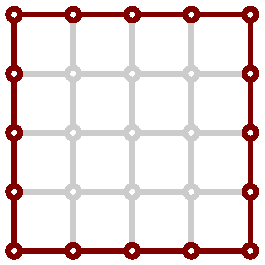
\includegraphics[width=3cm]{images/parallel_fiber_estimation/boundary_grid.pdf}%
   \caption{Grid of $4 \times 4$ boundary points, which occurs at the beginning of the procedure of \cref{alg:parallel_algorithm_1}.}%
    \label{fig:boundary_grid_1}%
  \end{subfigure}
  \quad
  \begin{subfigure}[t]{0.48\textwidth}%
    \centering%
    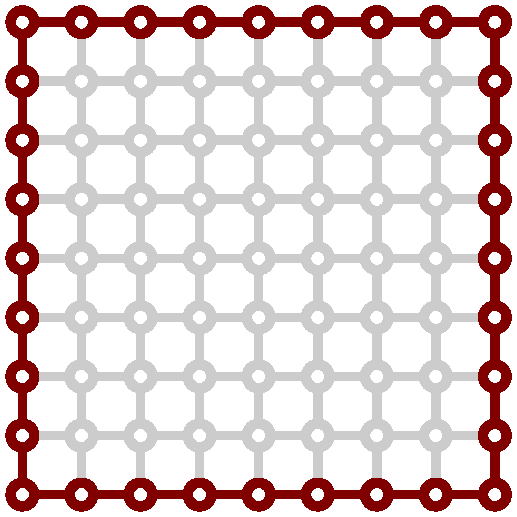
\includegraphics[width=3cm]{images/parallel_fiber_estimation/boundary_grid_2.pdf}%
    \caption{Grid with $4 \times 8$ boundary points, which occurs after a refinement step at beginning of the procedure of \cref{alg:parallel_algorithm_1}.}%
    \label{fig:boundary_grid_2}%
  \end{subfigure}   
  \caption{Logical subdomain boundaries (red) and interior grid (gray) before and after the refinement at the beginning of \cref{alg:parallel_algorithm_1}.}%
  \label{fig:boundary_grid}%
\end{figure}%

% refine border points
As the goal on every recursion level is to construct a mesh with half the mesh width of the mesh on the previous level, the given boundary points are refined to twice the amount by inserting new points at the centers between neighboring points. The refinement happends in all three coordinate directions. For the example with $n_\text{el,x}=4$, the resulting grid with the $4\times 8$ refined boundary points is shown in \cref{fig:boundary_grid_2}. In $z$ direction, we get $(2\,n_\text{el,z}+1)$ slices with points.

% logical structure of new subdomains
The task in the recursive procedure is now to determine boundaries for eight subdomains. This is achieved by subdividing the given 2D slices into four 2D subdomains each. Additionally, the 3D volume is split at its vertical center. Thus, the upper and lower parts contain four subdomains each. 
\Cref{fig:subdomain} visualizes this scheme for the eight subdomains on recursion level $l=1$. The boundary points of the first and the eighth subdomain are shown. The boundary points have already been refined such that every slice in \cref{fig:subdomain} consists of $4 \times 8$ points and corresponds to the grid in \cref{fig:boundary_grid_2}
\begin{figure}%
  \centering%
  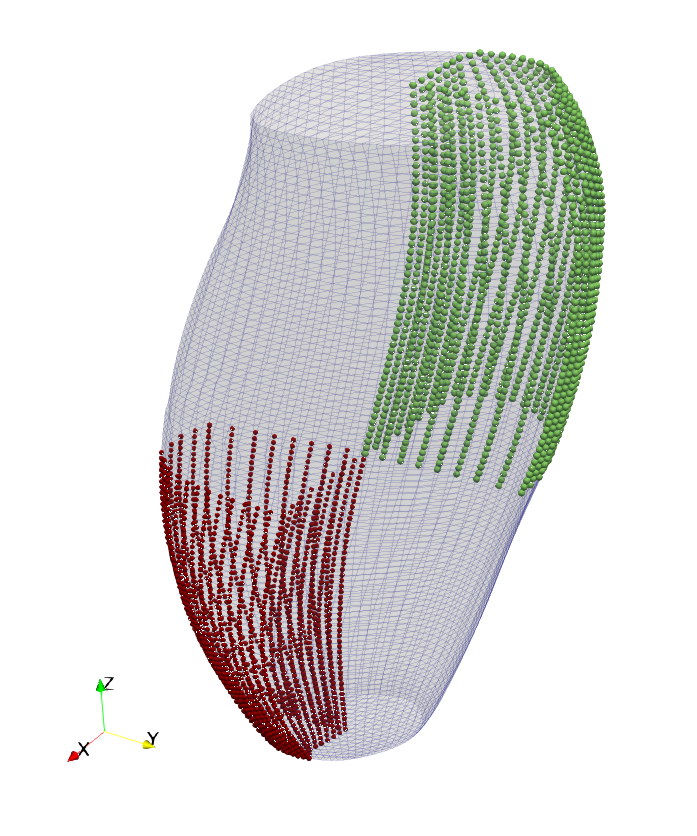
\includegraphics[height=8cm]{images/parallel_fiber_estimation/subdomains_2.png}%
  \caption{Parallel 3D mesh generation: Partitioning of the muscle volume into eight subdomains during the first call to the procedure in \cref{alg:parallel_algorithm_1}. The first (red) and the eighth subdomain (green) are shown.}%
  \label{fig:subdomain}%
\end{figure}%

%   ^v^v^

%For this reason, the given $4 \times 4$ boundary points are refined to twice the amount of boundary points by inserting new points at the centers between neighboring points. The resulting grid is shown in \cref{fig:boundary_grid_2}. Now, it would be possible to subdivide the grid to obtain four instances of the needed grid in \cref{fig:boundary_grid_1}.
%However, this would result in constant straight connection lines between the initial boundary points. In all further recursive calls, the additional points would all be placed on these lines and thereby not properly refine the subdomain boundaries. Instead, a different approach is desired where the subdomain's boundaries in the volume follow the directions of streamlines and fibers. Thus, the approach is to define the subdomain boundaries in the interior of the global domain by traced streamlines and sample the outer boundaries from the surface triangulation with the desired mesh width. The required steps of this approach are discussed next.

% --

\subsection{Generation and Smoothing of the 3D Mesh}
% create 3D mesh

After the \code{boundary\_points} variables has been set, the next step of \cref{alg:parallel_algorithm_1} is to construct a 3D mesh in the domain.
In line \ref{line:3.2} of \cref{alg:parallel_algorithm_1}, the harmonic map  algorithm \cref{alg:serial_algorithm_1} described in \cref{sec:ser_alg_meshes} is called. Its input consists of the boundary points that define the 2D slices of the volume. This means that \cref{alg:serial_algorithm_1} does not need to construct the slice boundary rings from the surface triangulation, instead, the formulation of \cref{alg:serial_algorithm_1} can directly start with line \ref{alg:1.2} to triangulate the slices and then compute the harmonic map. For the harmonic map computation, the second triangulation method is used with a circular reference domain quandrangulated by the second scheme. The result is a set of quadrangulated 2D slices that forms a 3D mesh by vertically connecting the elements of neighbor slices.

% smoothing
Next, line \ref{line:3.3} of \cref{alg:parallel_algorithm_1} improves the mesh quality of the 2D muscle slices $S_M$ from which the 3D mesh is formed. This action consists of two steps. The first step is to ensure that no self-intersecting or degenerate quadrilaterals exist in the slice. The second step applies Laplacian smoothing to improve the mesh quality of the slice.

Theoretically, the first step should not be necessary, as the chosen quadrangulation algorithm always produces valid elements. However, in practice, small or irregularly shaped, concave domains occur and together with rounding and numerical errors in the Laplace problem computations occasionally lead to invalid meshes with self intersecting elements, especially for higher recursion depths in \cref{alg:parallel_algorithm_1}. Executing the first step therefore increases the robustness of the implementation.

\begin{figure}%
  \centering%
  \def\svgwidth{0.7\textwidth}%
  \input{images/parallel_fiber_estimation/quads.pdf_tex}%
  \caption{Decomposition of quadrilateral elements into triangles as substep of the validity check of muscle slice quadrangulations. A quadrilateral element (left) and the four triangles (right) that can be constructed from its four points. These triangles are needed for the check in \cref{alg:parallel_algorithm_1} whether the quadrilateral element is valid.}%
  \label{fig:quads_tris}%
\end{figure}%

\begin{figure}%
  \centering%
  \begin{subfigure}[t]{0.48\textwidth}%
    \centering%
    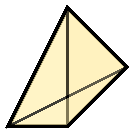
\includegraphics[width=3cm]{images/parallel_fiber_estimation/triangle_score_3.pdf}%
    \caption{Convex quadrilateral with score $s=4$ and the contained triangles, which are all oriented counterclockwise.}%
    \label{fig:triangle_score_3}%
  \end{subfigure}
  \quad
  \begin{subfigure}[t]{0.48\textwidth}%
    \centering%
    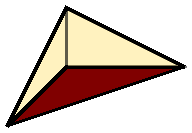
\includegraphics[width=3cm]{images/parallel_fiber_estimation/triangle_score_4.pdf}%
    \caption{Concave quadrilateral with score $s=3$ and the contained triangles. Only the red triangle is oriented clockwise.}%
    \label{fig:triangle_score_4}%
  \end{subfigure}   
  \caption{Check for valid elements in the muscle slice quadrangulations that occurs in \cref{alg:parallel_algorithm_1}: Illustration of the score of valid concave and convex quadrilaterals.}%
  \label{fig:triangle_score}%
\end{figure}%

The algorithm performs this step by repeatedly iterating over all interior mesh points in every slice $S_M$ and fixing invalid elements. To find invalid elements, for every quadrilateral the four triangles that can be formed from the points of the quadrilateral are considered, as shown in \cref{fig:quads_tris}.
For every triangle with points $\bfp^0,\bfp^1$ and $\bfp^2$, the orientation of the triangle is determined. The orientation is counterclockwise if the oriented triangle area $A_{012}$ is positive. The oriented triangle area is the determinant of the $3 \times 3$ matrix that contains the row vectors $(p^i_x,p^i_y,1)$ for the triangle points $\bfp^i=(p^i_x,p^i_y)^\top$ and can be computed by the following formula \cite{sedgewick2011algorithms}:
%
\begin{align*}
  A_{012} = (p^1_x-p^0_x)\,(p^2_y-p^0_y) - (p^2_x-p^0_x)\,(p^1_y-p^0_y).
\end{align*}
If the orientation is counterclockwise, a score value of the triangle is set to one, if it is clockwise, the score is set to zero. The score values of the four triangles are added up to yield a score $s$ for the quadrilateral. Only if this score is $s \geq 3$, the quadrilateral is valid. \Cref{fig:triangle_score} illustrates the cases of valid quadrilateral elements. In a valid, convex element, all four triangles lie inside the element and, thus, the score is $s=4$. If only one triangle is located outside, the quadrilateral is also valid and concave. In this case the score has the value $s=3$.

At the current mesh point in the loop over all points that are not at the boundary of the mesh, the four adjacent quadrilaterals are considered. If any of them is invalid, the algorithm tries to improve the situation by deflecting the point by a random, small vector. A maximum of 200 random deflections from the original position with exponentially increasing deflection vector sizes are tried. After each modification of the point, the scores of the four adjacent quadrilateral elements are evaluated. If the sum of the four element scores increases, the point is kept and the iteration over all interior mesh points starts anew. 

Note that this does not necessarily mean that the invalid element was fixed, only its score was improved. If it was not fixed, it will be considered again in the next iteration. For example, a convex element that initially is oriented clockwise instead of counterclockwise has a score of $s=0$. In the first iteration, one point is deflected such that the quadrilateral intersects itself but has a higher score $s\geq 0$. At least one more iteration is needed until the quadrilateral is oriented correctly.
When all elements in the slice $S_M$ are valid, this step is complete.

\subsection{Laplacian Smoothing}
The second step is the smoothing step that improves the mesh quality of the 2D slices. \num{20} iterations of Laplacian smoothing \cite{field1988laplacianSmoothingAndDelaunayTriangulations} are executed. Laplacian smoothing in our case subsequently visits all interior points of the mesh and sets the location of a point to the center of gravity of its four direct neighbors.
%The order in which the points of the mesh are traversed is changed after every iteration: In the first iteration, the points are traversed starting at the bottom left. In the second iteration, the traversal starts at the top right and moves in opposite direction compared to the first iteration. The third and fourth iterations begin at the bottom right and top left nodes of the mesh. After these four iterations the scheme is repeated. The reason for this change of the traversal is to 
\Cref{fig:laplace_smoothing} shows the effect of Laplacian smoothing for a slice in a subdomain on the first recursion level. It can be seen how the smoothing equalizes the element side lengths and angles.

However, this smoothing step can invalidate a mesh by introducing overlapping quadrilaterals. An example for this case is given in \cref{fig:laplace_smoothing_0}. The initial mesh in \cref{fig:world_mesh_0} is concave and occurs during recursion level $l=2$. \Cref{fig:world_mesh_improved_0} shows the result of the smoothing, which contains one invalid element. The smoothing operation placed the fourth point of the element that also contains the three boundary points at the concavity outside of the mesh. As a remedy, the smoothing method checks the validity of the adjacent elements before a point is moved. If the move would result in an invalid element, the action is not carried out and the traversal continues with the next point instead.
\Cref{fig:world_mesh_improved_1} shows the resulting mesh if this check is enabled. The mesh has slightly different boundaries because the check influenced the behavior already on lower recursion levels.

% smoothing fix

\begin{figure}%
  \centering%
  \begin{subfigure}[t]{0.48\textwidth}%
    \centering%
    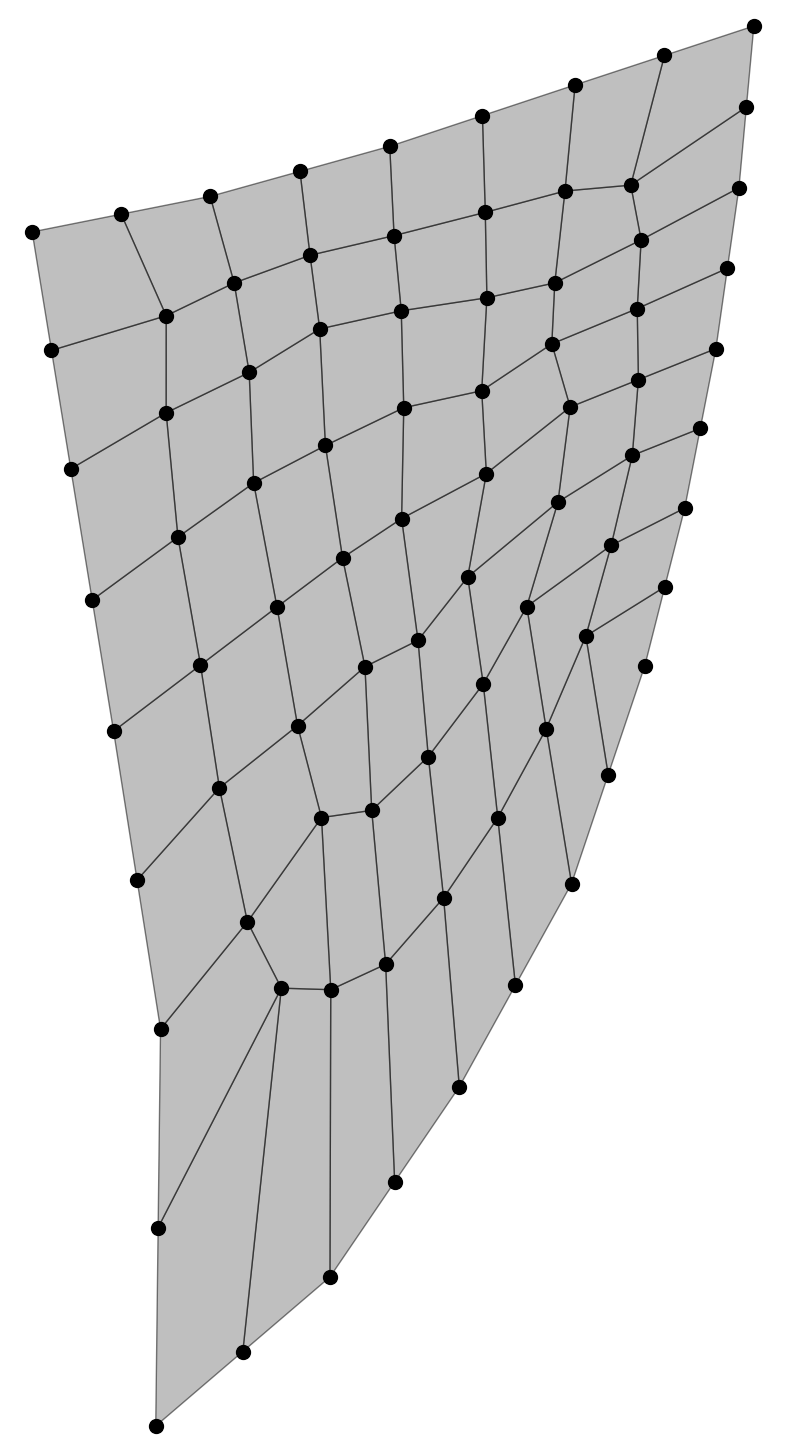
\includegraphics[height=7cm]{images/parallel_fiber_estimation/world_mesh.png}
    \caption{Initial 2D mesh of a subdomain at the boundary of the biceps muscle.}%
    \label{fig:world_mesh}%
  \end{subfigure}
  \quad
  \begin{subfigure}[t]{0.48\textwidth}%
    \centering%
    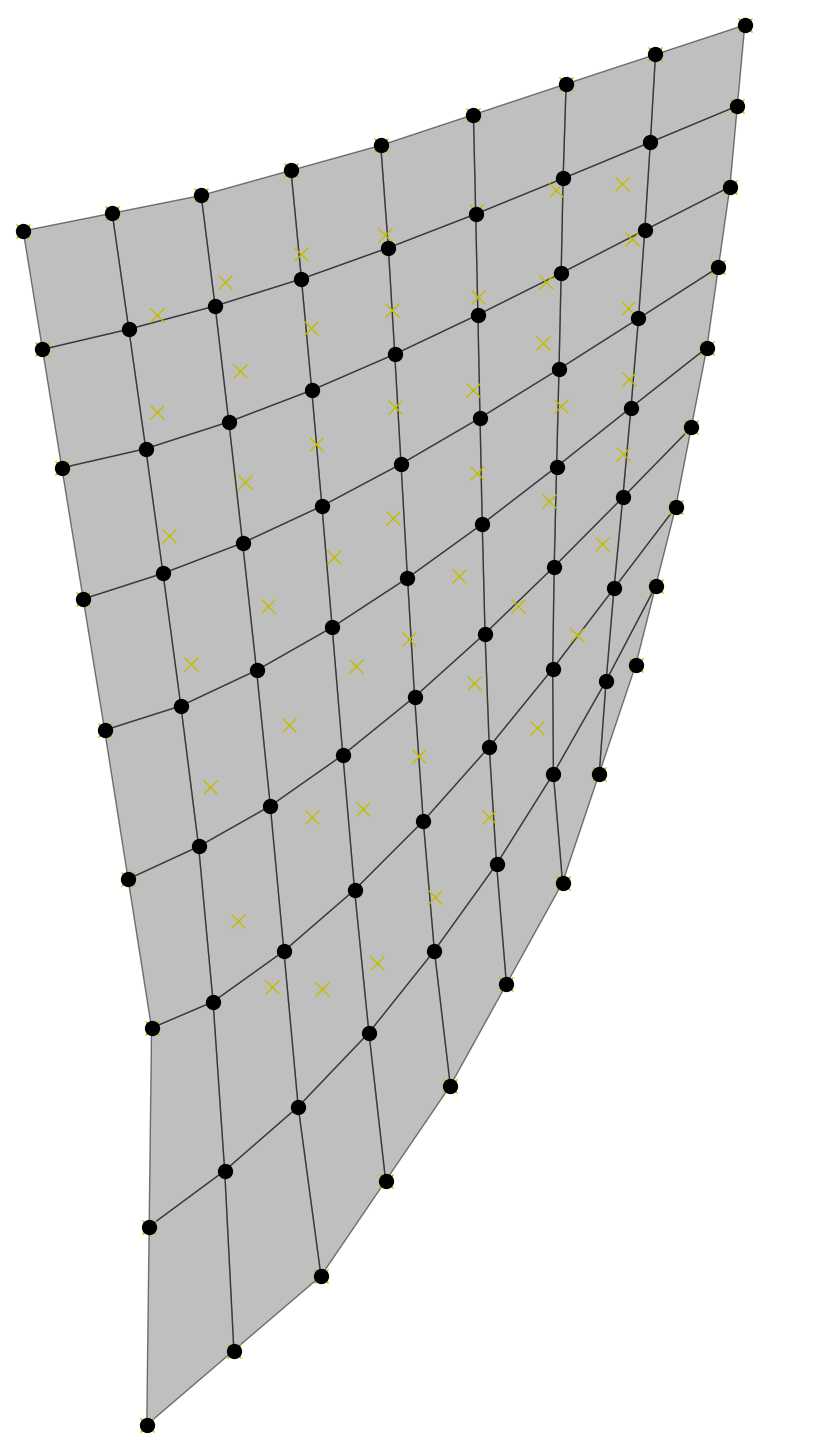
\includegraphics[height=7cm]{images/parallel_fiber_estimation/world_mesh_improved.png}
    \caption{The mesh of (\subref{fig:world_mesh}) after 20 iterations of Laplacian smoothing.}%
    \label{fig:world_mesh_improved}%
  \end{subfigure}    
  \caption{Quality improvement of 2D muscle slice quadrangulation: Effect of Laplacian smoothing of a 2D grid which occurs in line \ref{line:3.3} of \cref{alg:parallel_algorithm_1}.}%
  \label{fig:laplace_smoothing}%
\end{figure}%

\begin{figure}%
  \centering%
  \begin{subfigure}[t]{0.30\textwidth}%
    \centering%
    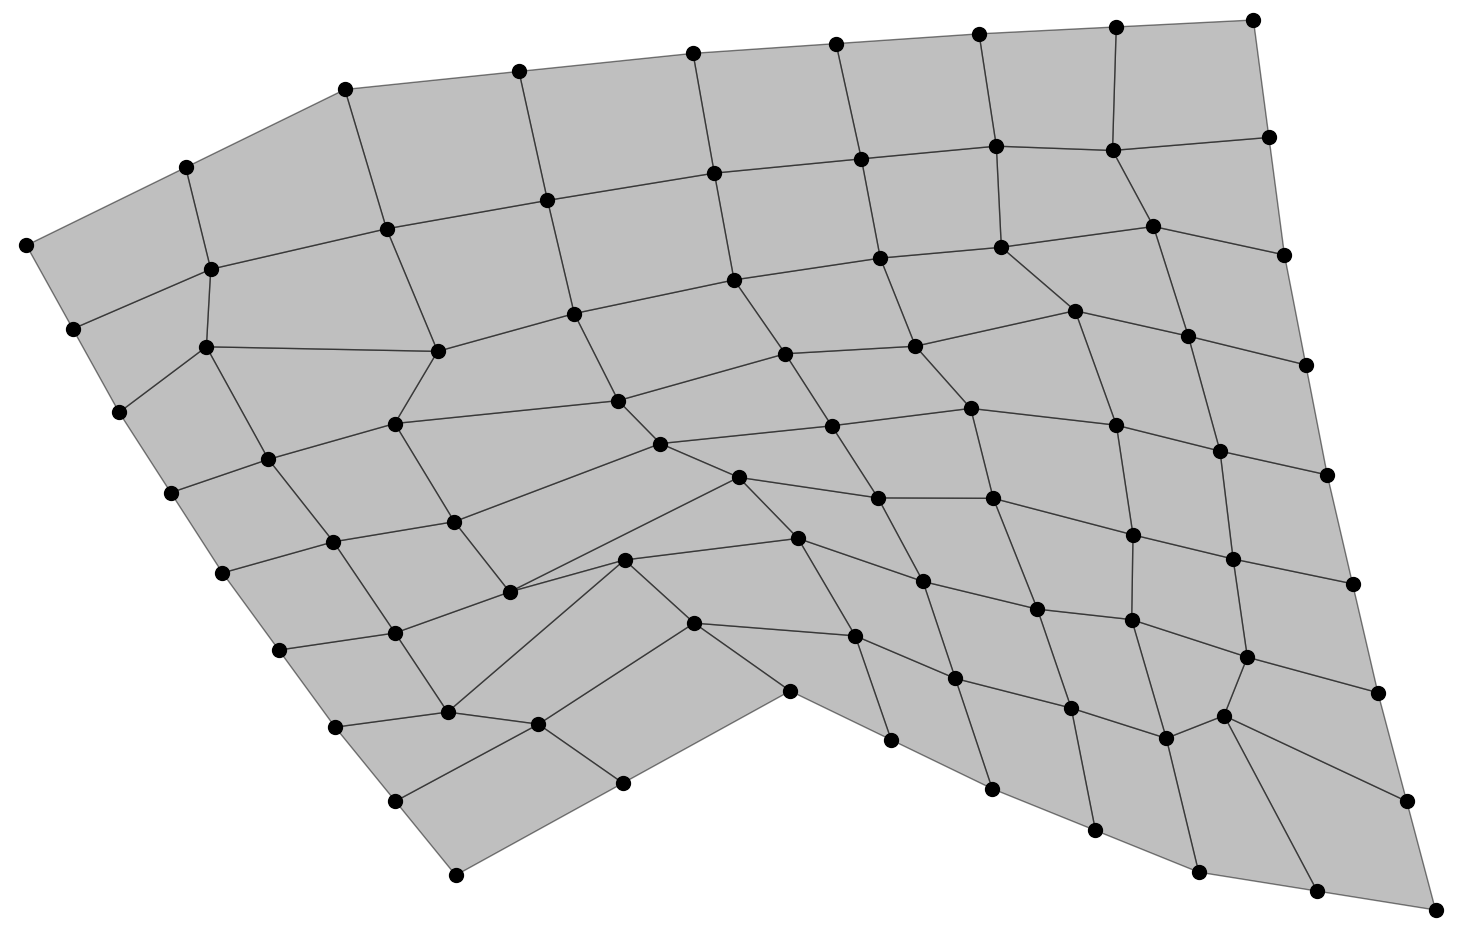
\includegraphics[width=\textwidth]{images/parallel_fiber_estimation/loop_025_p3728344_world_mesh.png}
    \caption{Initial 2D mesh.}%
    \label{fig:world_mesh_0}%
  \end{subfigure}
  \quad
  \begin{subfigure}[t]{0.30\textwidth}%
    \centering%
    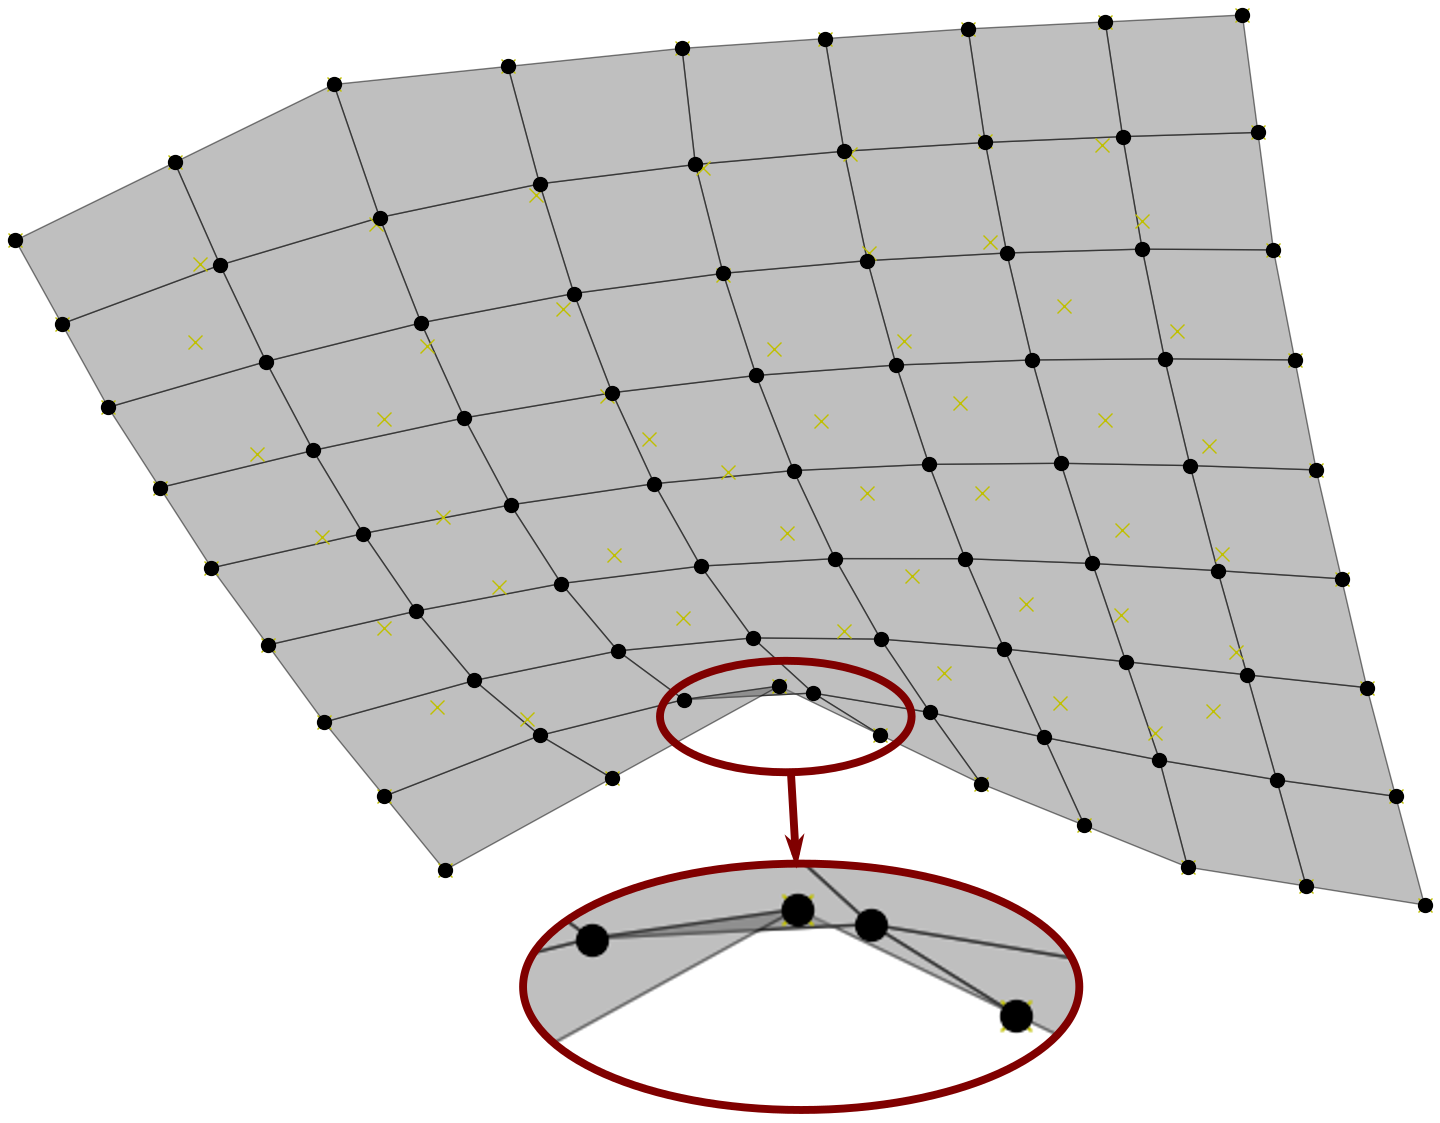
\includegraphics[width=\textwidth]{images/parallel_fiber_estimation/loop_025_p3728344_world_mesh_improved_3.png}
    \caption{The mesh of (\subref{fig:world_mesh_0}) after 20 iterations of Laplacian smoothing, yielding an invalid quadrangulation.}%
    \label{fig:world_mesh_improved_0}%
  \end{subfigure}    
  \quad
  \begin{subfigure}[t]{0.30\textwidth}%
    \centering%
    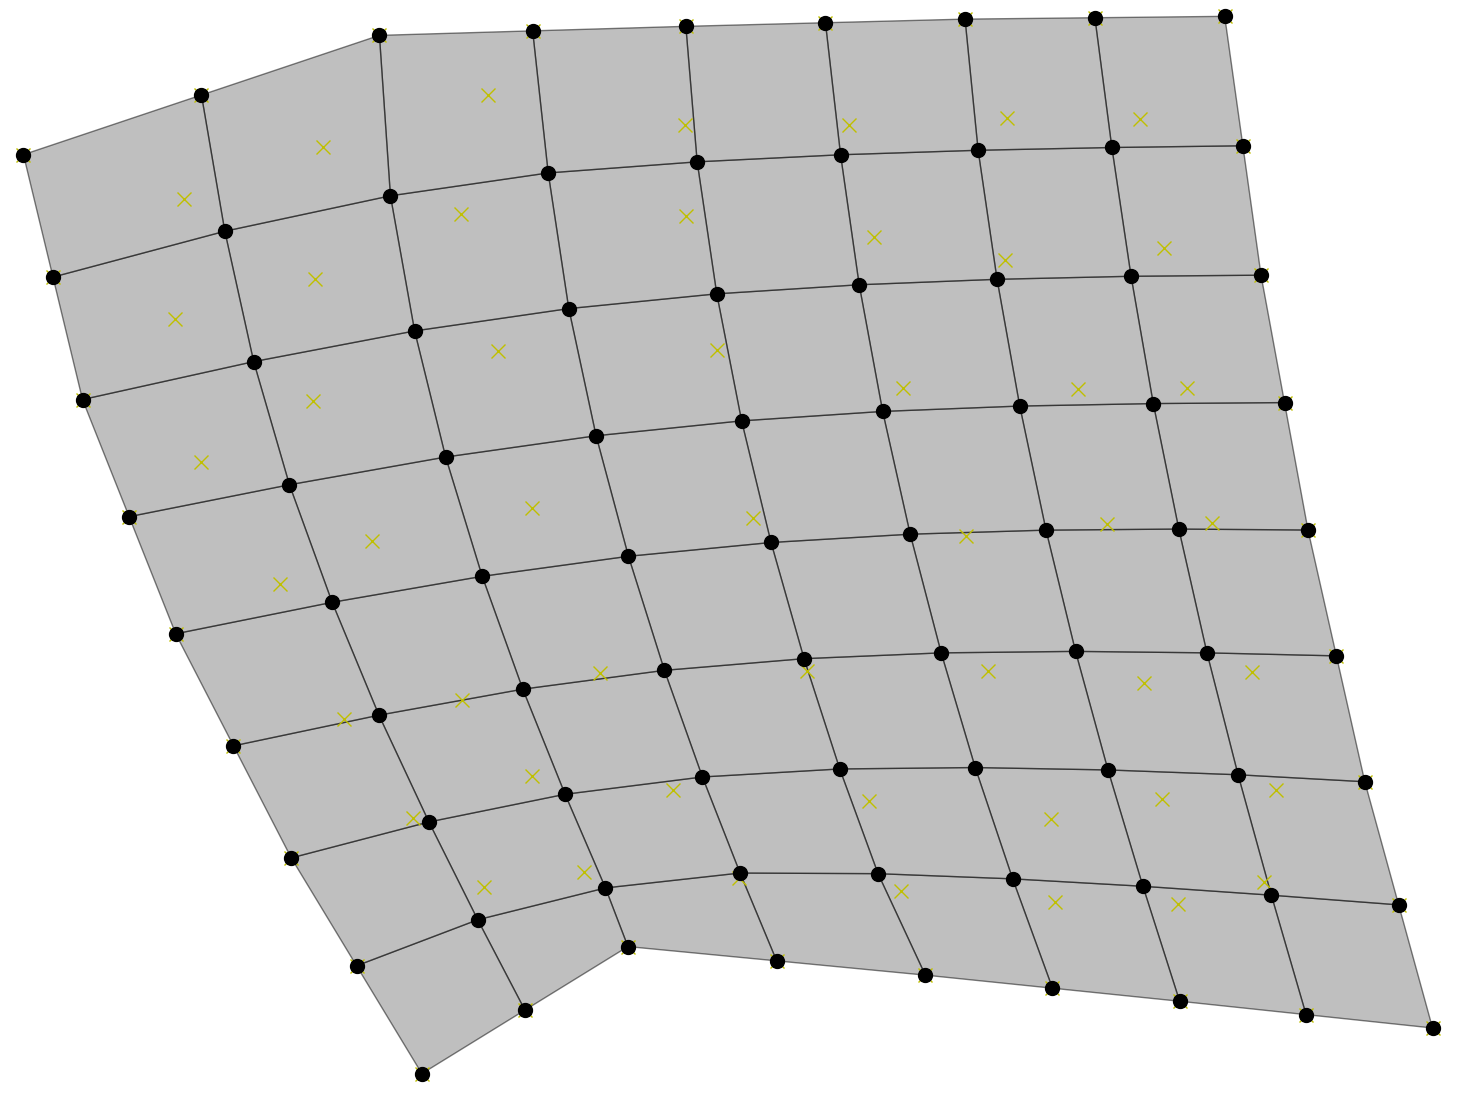
\includegraphics[width=\textwidth]{images/parallel_fiber_estimation/loop_025_p30402_world_mesh_improved.png}
    \caption{The mesh of (\subref{fig:world_mesh_0}) after 20 iterations of Laplacian smoothing with the validity check, yielding a valid quadrangulation.}%
    \label{fig:world_mesh_improved_1}%
  \end{subfigure}    
  \caption{Quality improvement of 2D muscle slice quadrangulation: Effects of Laplacian smoothing on concave domains.}%
  \label{fig:laplace_smoothing_0}%
\end{figure}%

\subsection{Solution of the Laplace Problem}\label{sec:solution_of_the_laplace_problem}

After the 3D mesh has been created and smoothened, the next steps are to solve the Laplace problem in the muscle domain, to trace streamlines in the gradient of the solution vector field and finally to construct the eight subdomains for the recursive calls by subdividing the own domain along the streamlines.

% refine 3D mesh
Prior to the solution of the Laplace problem, the 3D mesh gets refined further by increasing the number of elements per coordinate direction by a specified factor $r\in \N$. The rationale is to increase the number of degrees of freedom and, thus, the resolution to get a smaller numerical error in the subsequent Laplace computation.
This refinement is in addition to the refinement of the initial boundary points by a factor of two described in \cref{sec:data_structure_of_boundary_points}. The mesh with $2\,n_\text{el,x} \times 2\,n_\text{el,x} \times 2\,n_\text{el,z}$ elements gets refined to $2\,r\,n_\text{el,x} \times 2\,r\,n_\text{el,x} \times 2\,r\,n_\text{el,z}$ elements. The new points are found by interpolating in the existing mesh.

For example, the 3D mesh of \cref{fig:boundary_grid} with $2\cdot 4 \times 2\cdot 4 \times 2\cdot 50$ elements gets refined with the factor $r=2$ to $16 \times 16 \times 200$ elements.
\Cref{fig:02_boundary_points} shows the refined boundary points in this example in a view in negative $z$ direction towards the bottom of the muscle. The red points are the boundary points of the $4 \times 8$ grid, the additional white points are added in between by the refinement with $r=2$. 
Because this refinement is carried out by interpolating between the initial points, the new points are located on straight lines between the initial points.
This can especially be seen at the lower left of the figure (indicated by arrows and lines) where always five neighboring points lie on a straight line. 

\begin{figure}%
  \centering%
  \begin{subfigure}[t]{0.45\textwidth}%
    \centering%
    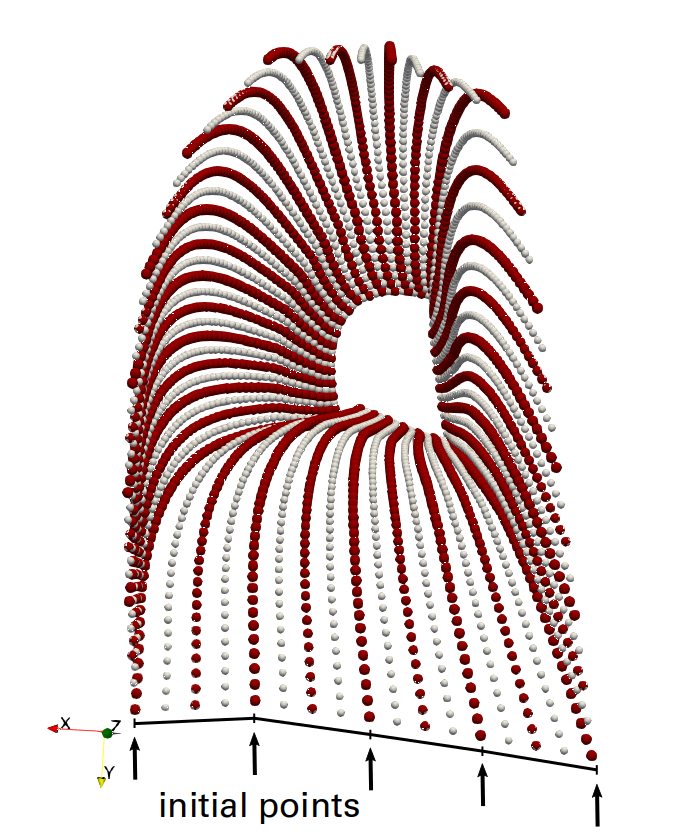
\includegraphics[height=9cm]{images/parallel_fiber_estimation/02_boundary_points_2.png}
    \caption{Initial (arrows) and refined boundary points (red) and points after additional refinement by a factor of $r=2$ (white).}%
    \label{fig:02_boundary_points}%
  \end{subfigure}   
  \quad
  \begin{subfigure}[t]{0.45\textwidth}%
    \centering%
    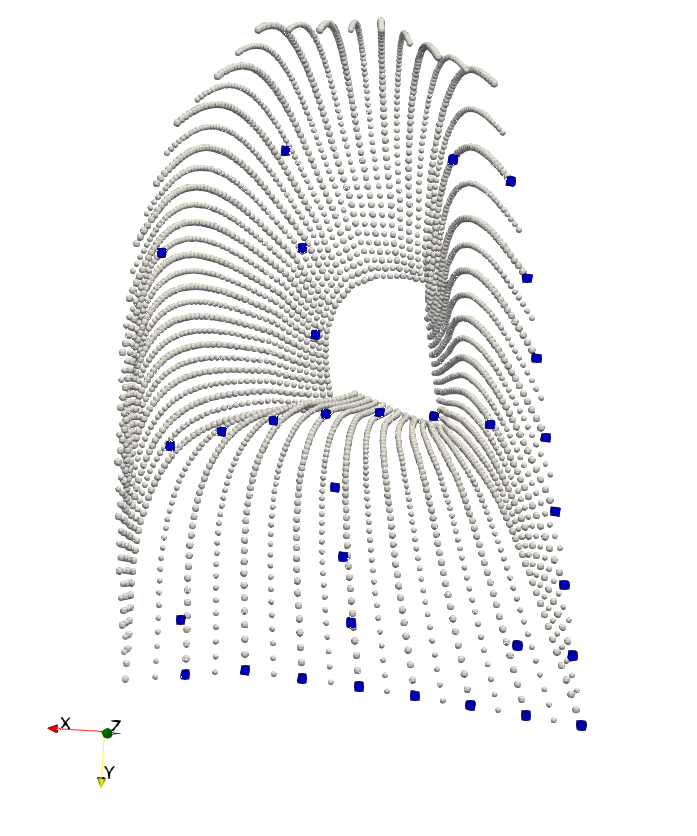
\includegraphics[height=9cm]{images/parallel_fiber_estimation/03_seed_points.png}
    \caption{Seed points for the streamlines (blue).}%
    \label{fig:03_seed_points}%
  \end{subfigure}
  \\
  \begin{subfigure}[t]{0.45\textwidth}%
    \centering%
    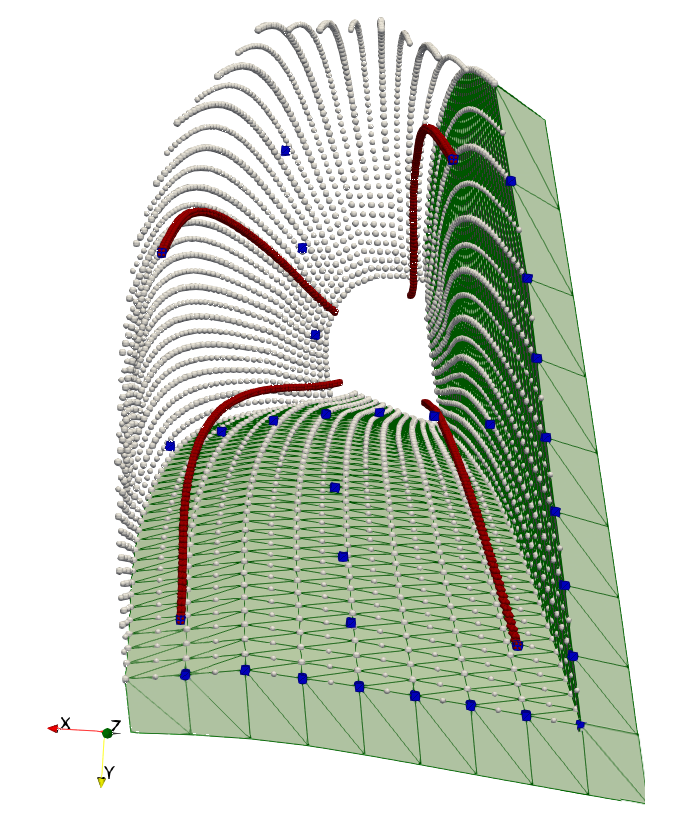
\includegraphics[height=8cm]{images/parallel_fiber_estimation/05_corner_streamlines_corner.png}
    \caption{The four boundary streamlines (red) and the layer of ghost elements (green) at the bottom and right of the subdomain.}%
    \label{fig:05_corner_streamlines}%
  \end{subfigure}   
  \quad
  \begin{subfigure}[t]{0.45\textwidth}%
    \centering%
    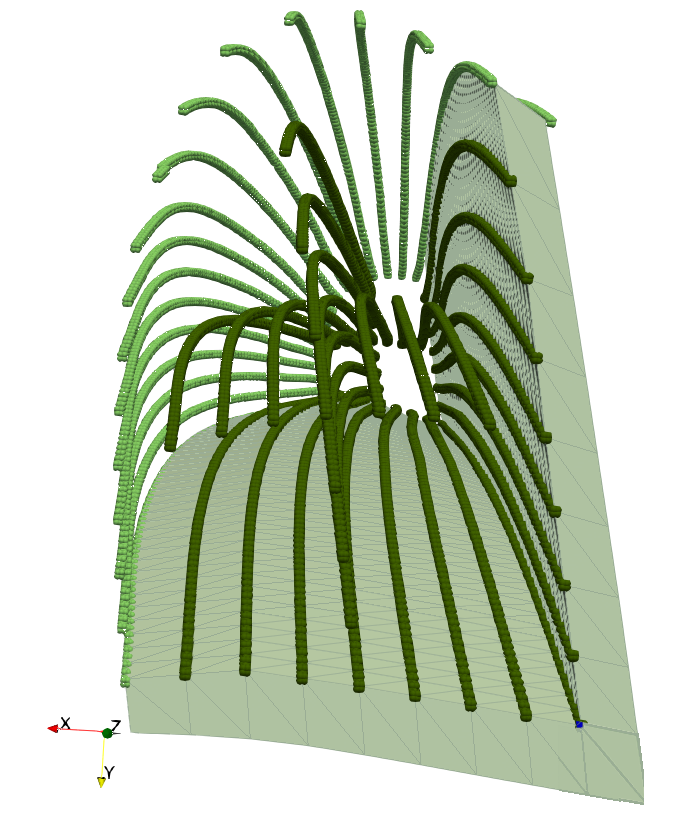
\includegraphics[height=8cm]{images/parallel_fiber_estimation/07_filled_corner.png}
    \caption{New boundary points on the outer (light green) and interior boundary (dark green).}%
    \label{fig:07_filled}%
  \end{subfigure}  
  \caption{Parallel generation of 3D meshes: refined boundaries, streamlines and subdomain refinement in the first subdomain for recursion level $l=1$.}%
  \label{fig:03_boundary_points_and_seed_points}%
\end{figure}%

% laplace problem
Next, in line \ref{line:3.4} of \cref{alg:parallel_algorithm_1} the Laplace problem gets solved. The same step also occurs in \cref{alg:serial_algorithm_2} and is explained in \cref{sec:generation_of_fiber_meshes}.
The equation is formulated globally and the discretization uses the existing partitioning. 
Dirichlet boundary conditions of $p(\bfx) = 0$ and $p(\bfx) = 1$ are prescribed at the bottom and top of the domain, as shown by the spheres in \cref{fig:dirichlet_bc_1}. Alternatively, Neumann boundary conditions can be used.
A parallel GMRES solver is employed to obtain the solution in a small number of iterations. E.g., for the biceps muscle the a linear system at $l=0$ has 4131 degrees of freedom and 26 iterations are needed to obtain a residual norm below \num{1e-4}. After the solution $p(\bfx)$ is obtained, the gradient field $\nabla p(\bfx)$ is computed. The solution and the gradient directions are visualized in \cref{fig:laplace_1}.

\begin{figure}
  \centering
  \begin{subfigure}[t]{0.23\textwidth}%
    \centering%
    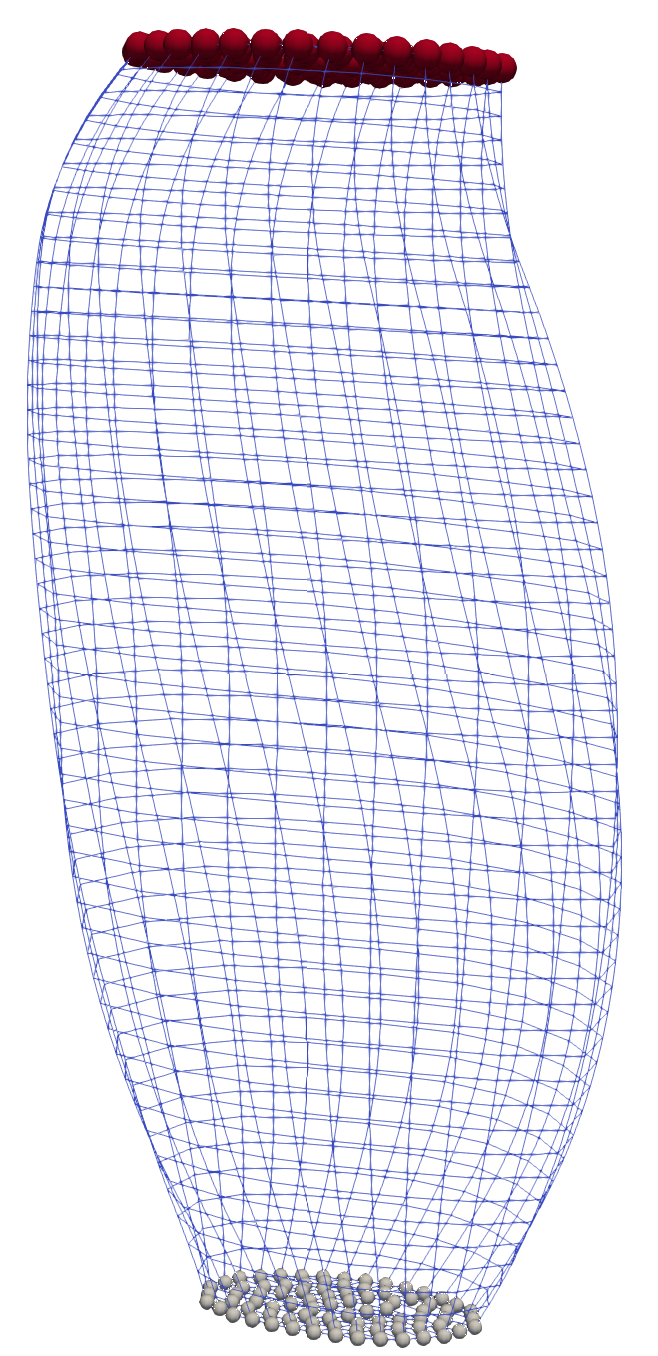
\includegraphics[height=7cm]{images/parallel_fiber_estimation/dirichlet_bc_1.png}
    \caption{Location of Dirichlet boundary condition nodes at the bottom and top.}%
    \label{fig:dirichlet_bc_1}%
  \end{subfigure}
  \,
  \begin{subfigure}[t]{0.24\textwidth}%
    \centering%
    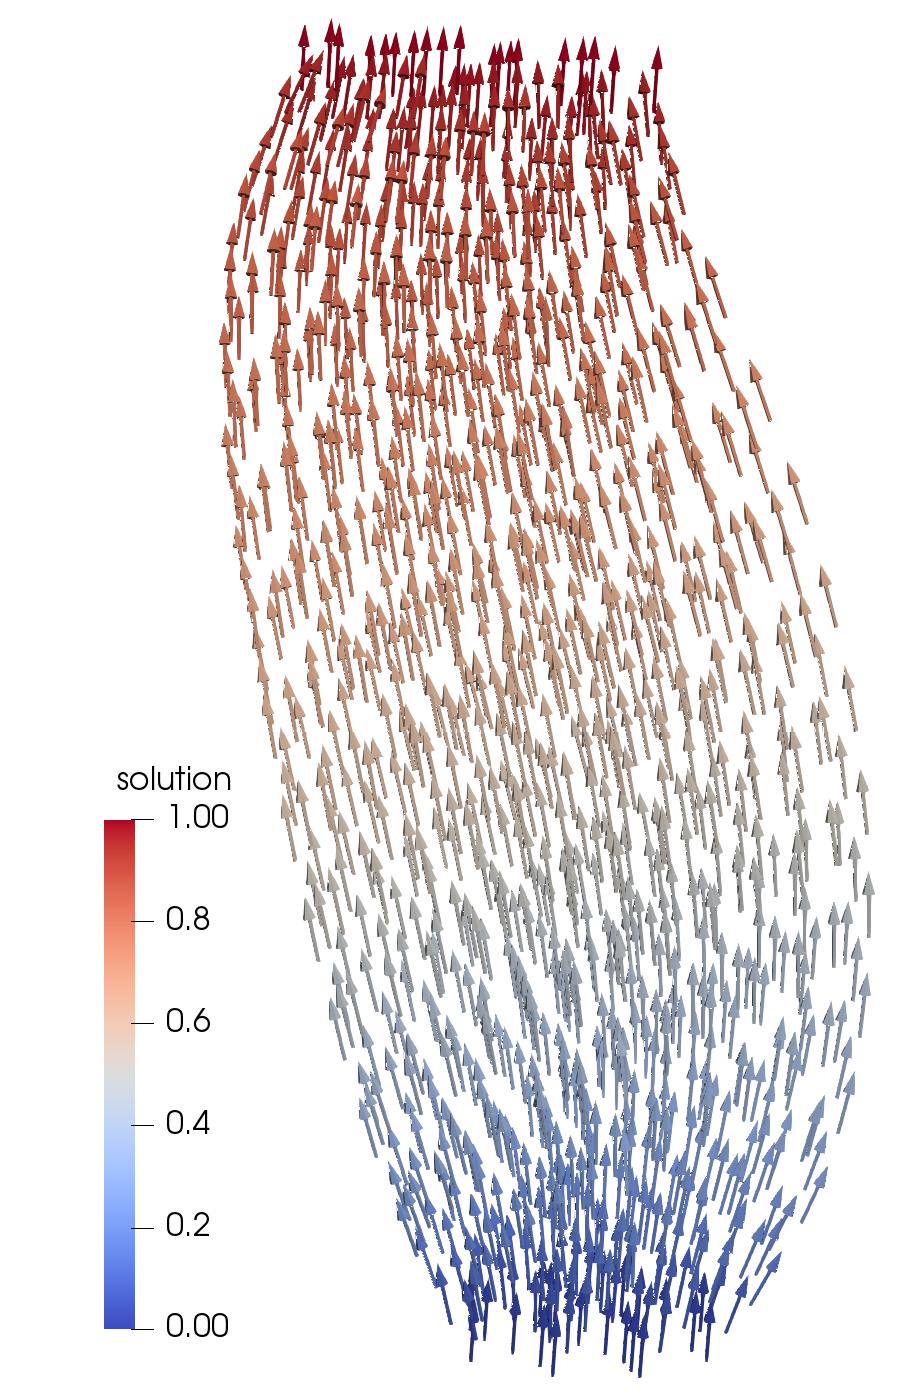
\includegraphics[height=7cm]{images/parallel_fiber_estimation/laplace_1.png}
    \caption{Solution $p$ of the Laplace problem and direction of the gradient $\nabla p$.}%
    \label{fig:laplace_1}%
  \end{subfigure}
  \qquad
  \begin{subfigure}[t]{0.19\textwidth}%
    \centering%
    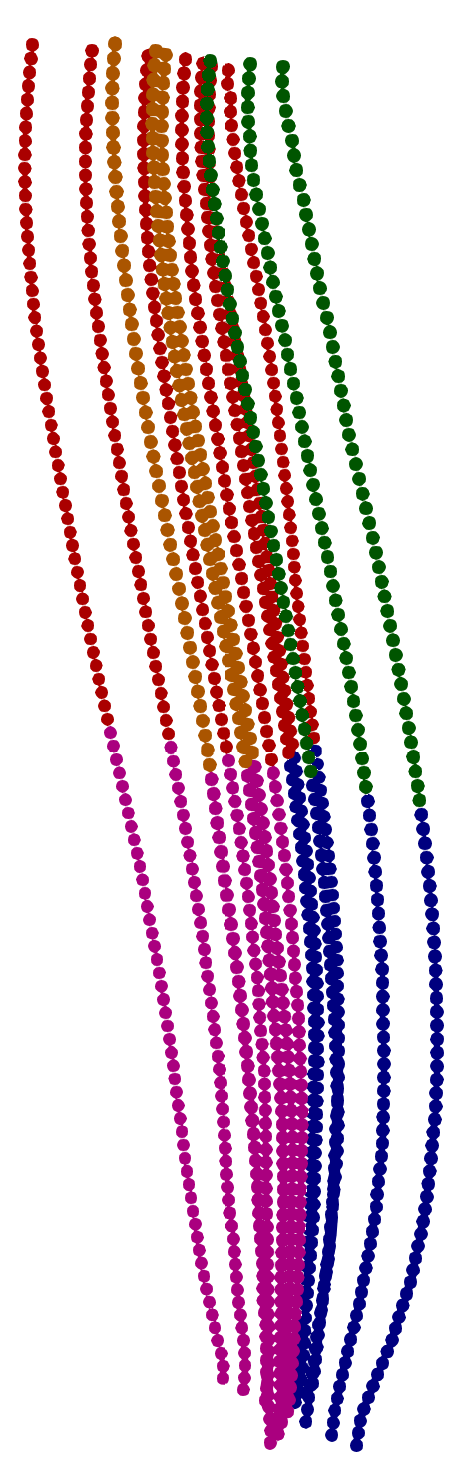
\includegraphics[height=7cm]{images/parallel_fiber_estimation/boundary_points_1.png}
    \caption{Traced streamlines that split the domain into eight subdomains.}%
    \label{fig:boundary_points_1}%
  \end{subfigure}
  \,
  \begin{subfigure}[t]{0.24\textwidth}%
    \centering%
    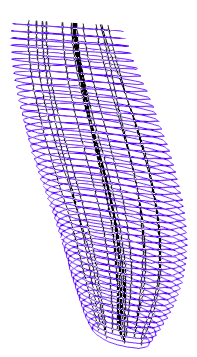
\includegraphics[height=7.2cm]{images/parallel_fiber_estimation/slices_2.png}
    \caption{Rings of the slices $S_M$ and traced streamlines in the interior.}%
    \label{fig:slices_2}%
  \end{subfigure}
  \caption{Parallel 3D mesh generation: Process of subdividing the muscle volume into eight subdomains using the solution of a Laplace problem, which is an important step in the procedure of \cref{alg:parallel_algorithm_1}.}
  \label{fig:determining_subdomains}%
\end{figure}

\subsection{Communication of the Ghost Layer}

% ghost communication
Subsequently, the gradient field $\nabla p(\bfx)$ is used to trace streamlines to determine new boundaries of the subdomain. This involves tracing streamlines that start exactly on the boundary. These streamlines potentially switch between the subdomain owned by the current process and the subdomains of neighboring processes. Streamline tracing requires the gradient field values of the elements where the streamline passes through.
To avoid repeated communications in these cases, a ghost layer of a specified number $n_\text{ghost\_layer\_width}$ of elements is added to the subdomains at all parts of the boundary that touch a neighboring subdomain directly or diagonally adjacent in $x$ and $y$ direction.

The ghost layer is constructed and the node positions and values of $p$ and $\nabla p$ associated with the ghost elements are communicated between the neighboring processes after the solution of the Laplace problem.
This occurs in line \ref{line:3.5} of the algorithm. \Cref{fig:05_corner_streamlines} shows $n_\text{ghost\_layer\_width}=1$ layer of ghost elements on a subdomain at recursion level $l=1$.

\subsection{Selection of Seed Points for the Streamlines}\label{sec:selection_of_seed_points}

% seed points-1
Next, the seed points from which the streamlines start are determined on the subdomain.
All seed points are selected from the set of nodes in the structured mesh of a horizontal 2D slice. 

\Cref{fig:seed_points_to_send_1} visualizes the structured mesh in light gray in the first call to the procedure for recursion level $l=0$ where the domain is not yet partitioned.
The selected seed points are shown by the yellow and red points.
As can be seen, the seed points consist of the nodes of the 2D mesh at the horizontal and vertical centers in this view which form the \emph{plus sign} shape given by the yellow points.
In addition, the four red points near the corners of the structured mesh are selected.
%\Cref{fig:seed_points_to_send_1} also visualizes the boundary of the slice together with a method of splitting it into eight sectors by choosing the splitting points such that they are the closest to the given outer seed points.

% seed points interior for l=0
The seed points of the \emph{plus sign} yield the streamlines that subdivide the domain into four parts in $x$ and $y$ direction. With the additional split in $z$ direction, the inner boundaries of the eight subdomain are obtained. The resulting boundaries are given in \cref{fig:fixed_1}.

The streamlines of these seed points are also depicted in \cref{fig:boundary_points_1}. The interior boundary points for the eight subdomains that partition the muscle volume at level $l=1$ are shown by different colors.
The full subdomain boundaries include also the outer surface of the muscle, which is given by the rings of the muscle slices.
\Cref{fig:slices_2} shows the streamlines in black and the circumferential rings of the muscle slices in blue that were extracted during the call to \cref{alg:serial_algorithm_1} in line \ref{line:3.2}. 


\begin{figure}
  \centering
  \begin{subfigure}[t]{0.30\textwidth}%
    \centering%
    %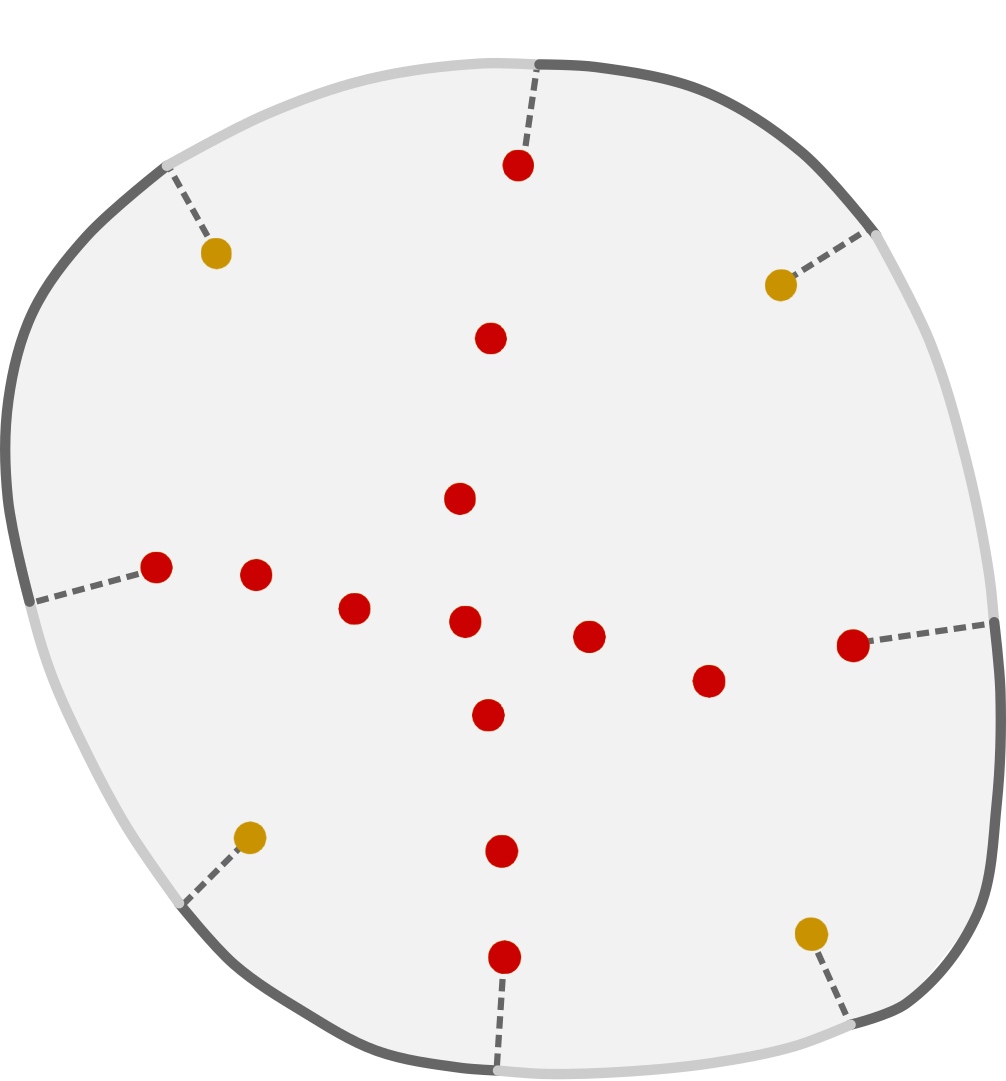
\includegraphics[height=4cm]{images/parallel_fiber_estimation/seed_points_to_send_1a.png}
    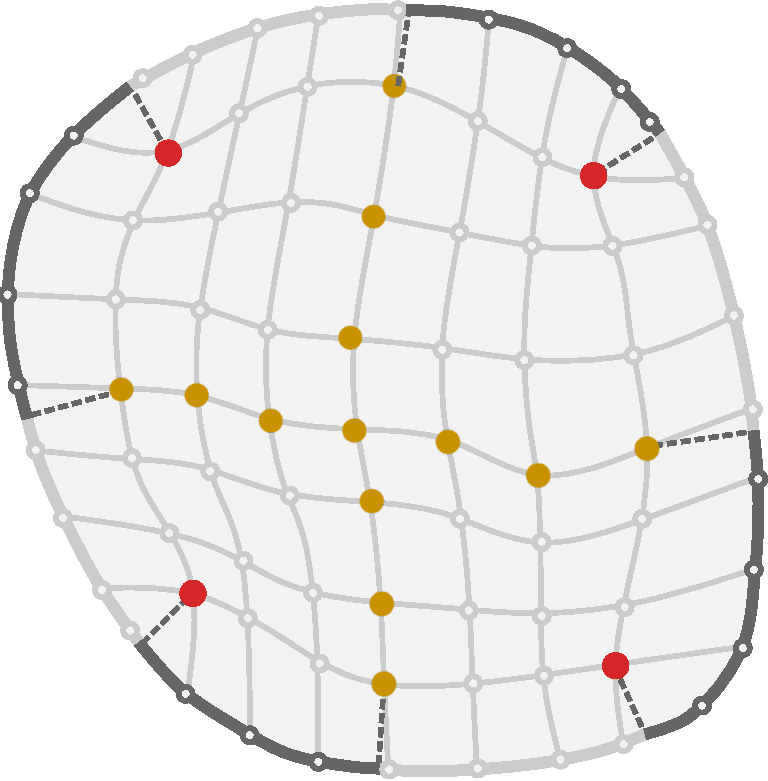
\includegraphics[height=5cm]{images/parallel_fiber_estimation/fixed_0.pdf}
    \caption{The seed points of the streamlines used to determine the subdomain boundaries. }%
    \label{fig:seed_points_to_send_1}%
  \end{subfigure}
  \,
  \begin{subfigure}[t]{0.30\textwidth}%
    \centering%
    
\includegraphics[height=5cm]{images/parallel_fiber_estimation/fixed_1.png}
    \caption{Streamlines and lines on the muscle surface that define the new subdomain boundaries.}%
    \label{fig:fixed_1}%
  \end{subfigure}
  \,
  \begin{subfigure}[t]{0.30\textwidth}%
    \centering%
    
\includegraphics[height=5cm]{images/parallel_fiber_estimation/final_interior_1.png}
    \caption{All streamlines and lines on the muscle surface that are created if the algorithm is run with one process and $l_\text{max}=0$.}%
    \label{fig:final_interior_1}%
  \end{subfigure}
  \caption{Parallel mesh generation: Seed points and streamlines that occur during the first call to the procedure in \cref{alg:serial_algorithm_2}, in a view from the top of the muscle.}
  \label{fig:seed_points}%
\end{figure}

% seed points interior for l>0
At higher recursion levels $l>0$, the boundaries for the new subdomains consist of those at the outer boundary of the muscle defined by the surface representation and those in the interior of the muscle.
Similar to the previously considered case at recursion level $l=0$, for $l\geq 1$ the boundaries in the interior of the muscle have to be sampled by a set of streamlines. In addition to the streamlines associated with the plus sign shaped seed points, new streamlines at the boundaries of the current subdomain have to be obtained.

\Cref{fig:03_seed_points} shows in blue all seed points that are selected in a subdomain on recursion level $l=1$ in order to create subdomain boundaries for level $l=2$.
As can be seen, in addition to the plus sign shape and the four outer seed points two lines of points in approximate $x$ and $y$ directions are selected at the lower and right edges of the image.
These are seed points for the new boundaries in the interior of the muscle. Note that the current recursion level $l=1$ also has boundaries at these locations. However, for level $l=2$ these boundaries are recreated by the new streamlines. Tracing of these streamlines potentially uses the ghost layer. The resulting streamlines and the ghost layer for $n_\text{ghost\_layer\_width}=1$ are shown in \cref{fig:05_corner_streamlines,fig:07_filled}.

\subsection{Determination of Subdomain Boundaries on the Outer Muscle Surface}

% seed points-3 outer ring
Next, the boundary points on the outer surface of the muscle are determined for the new partitioning. They are obtained by sampling the circumferential rings of the muscle surface with the resolution required in the current recursion level. In our implementation, this can be done either by sampling the original surface triangulation of the muscle or by directly evaluating the parametric form of the NURBS surface that approximiates the muscle surface.

At recursion level $l=0$, the entire muscle surface is touched by the new subdomains. Thus, when traversing the circumference of the muscle four new subdomains are encountered.
In consequence, every circumferential ring needs to be split into four quarter parts for the four adjacent subdomains. For each of these new subdomains, the quarter part corresponds to two neighboring sides of the subdomain boundary in \cref{fig:boundary_grid_1}. \Cref{fig:seed_points_to_send_1} also visualizes the two neighboring sides per new subdomain as dark and light portions of the outer boundary. 
To obtain these sides, a splitting point is needed that further splits every quarter part of the circumferential ring into the two sides for the new subdomain.
In summary, the ring needs to be split into eight parts that fit to the inner subdomain boundaries.

The eight split points are determined by the eight outer streamline points. In \Cref{fig:seed_points_to_send_1}, the four outer yellow points of the plus sign and the four red points are considered. For each split location, the nearest point on the circumferential ring is determined. The employed algorithm for calculating the coordinates of the point on a ring that has the shortest distance to a given, second point is described in \cref{sec:slicing_of_the_geometry}.

After the two sections of the circumferential rings have been determined for all new subdomains, the sections are equidistantly sampled in circumferential direction with $n_\text{el,x}$ elements each to create the outer boundary points for the subdomains. 
Also in longitudinal direction of the muscle, i.e., the $z$ axis, points are sampled on each streamline and on the outer boundary surface to yield the required number of $n_\text{el,z}$ points per subdomain. The resulting boundary points obtained during recursion level $l=0$ are shown in \cref{fig:fixed_1}.

This method is also required on higher recursion levels $l>0$ in a similar manner. 
Then, however, two cases have to be considered separately. The first case involves splitting the muscle surface boundary on one process into two parts, analogously to the described method at $l=0$. The second case involves two neighboring processes that have to agree on the split point of their common part of the outer surface boundary.

In the example at recursion level $l=1$ in \cref{fig:05_corner_streamlines}, the red streamlines are used to split the boundary sides at the outer boundary of the global domain. 
The first case occurs for the upper left red streamline, which is used to bisect the shown white part of the muscle surface. 

The second case occurs at the lower left and upper right borders between the shown subdomain and the neighboring subdomains of two other processes. For the case at the upper right, \cref{fig:seed_points_case_2} visualizes the following method: First, the point on the outer surface that is closest to the point of the red streamline is determined on both subdomains, visualized by the yellow stars. These points are communicated between the two processes. Each process computes the center point of these two points (orange star) and then finds the closest point to this center point on the boundary. This is done for all rings of the muscle in $z$ direction. In result, both processes have the same line on the surface in longitudinal direction of the muscle that is then used as one edge of the new subdomains.

\begin{figure}
  \centering
  \def\svgwidth{0.7\textwidth}
  \input{images/parallel_fiber_estimation/fixed_1.pdf_tex}
  \caption{Parallel mesh generation: Case of partitioning the outer boundary surface that occurs for recursion level $l \geq 1$ in \cref{alg:serial_algorithm_2}. Shown are the meshes on two subdomains of processes $p_0$ and $p_1$ and the location of the streamline at the corner (red points). The orange star is the newly determined border point between the subdomain boundaries.}
  \label{fig:seed_points_case_2}%
\end{figure}

Thus, the new subdomain boundaries on the outer boundary can be found using the red extra streamlines shown in \cref{fig:05_corner_streamlines}.
For simplicity, the algorithm always computes the four streamlines in every corner of the mesh although all of them are only required for $l=0$. In the shown example for $l=1$, the streamline in the lower right corner is not needed for the sampling of the new boundary points. 

A summary of the streamlines that are used for the new subdomain boundaries in this example is given in \cref{fig:07_filled}.
The sampled boundary points at the muscle surface are shown in light green color. These two sides of the own domain will be split into four sides for the new subdomains. In this example with $n_\text{el,x}=4$, the surface therefore gets sampled at $4\times 4=16$ lines. A comparison with the white lines in \cref{fig:05_corner_streamlines} shows that the newly sampled points are different from the initially sampled points. While in  \cref{fig:05_corner_streamlines} always five neighboring boundary points are located on a straight line, the points in \cref{fig:07_filled} follow the curved outer boundary better and, thus, refine the boundary representation.

\subsection{Parallel Algorithm for Streamline Tracing}\label{sec:parallel_streamline_tracing}
% streamline tracing method

In line \ref{line:3.6} of \cref{alg:parallel_algorithm_1}, streamlines have to be traced through the gradient field $\nabla p(\bfx)$ of the Laplace solution for all the seed points given in \cref{sec:selection_of_seed_points}. In the following, more details on the parallel method of streamline tracing is given.


This step is similar to the analog step in \cref{alg:serial_algorithm_2}. 
The same method of explicit Euler integration is used. The seed points are located at the horizontal plane at the center in vertical direction of the muscle. From there, streamlines are traced in both directions towards the ends of the muscle following the positive and negative gradient directions.
The tracing algorithm uses the efficient scheme of selecting the subsequently traversed elements described in \cref{sec:algorithm_for_streamline_tracing}. The implementation is adjusted in a way to also take into account the layers of ghost elements.

% streamline tracing in parallel-1
Since the streamlines traverse the entire muscle from the center to the bottom and top, multiple processes are involved in the computation of every streamline. To describe the scheme, all processes are numbered in $z$ direction from bottom to top by an index $i_z \in \{0, 1, \dots, n_z-1\}$ where $n_z = 2^l$ is the number of processes in $z$ direction on the current recursion level $l$.

% streamline tracing in parallel-2
The initial seed points are determined on the processes at the vertical center with index $\lfloor n_z/2\rfloor$. They are communicated to the processes below with index $\lfloor n_z/2\rfloor-1$. These two groups of processes begin with tracing the streamlines through their subdomains starting from the same seed points, the upper processes in upward and the lower processes in downward direction. Then, the end points of the traced streamlines are communicated to the next processes, which continue the tracing. The procedure repeats with further processes until the streamlines reach the bottom and top ends of the overall muscle domain.
The time complexity of this approach is $\O(n_z) = \O(\sqrt[3]{n_\text{proc}})$ with the number $n_\text{proc}$ of processes.

% streamline sampling
After the streamlines have been traced, they are sampled at equidistant positions with a distance according to the required distance between the boundary points of the subdomains.

\subsection{Recursion End: Generation of the Resulting Meshes}

% summary/überleitung
In result, one pass of \cref{alg:parallel_algorithm_1} from lines \ref{line:3.2} to \ref{line:3.7} creates boundaries for eight new subdomains. Line \ref{line:3.8} checks whether the maximum recursion $l_\text{max}$ is reached and the recursion ends. If the recursion ends, the final 3D mesh and 1D fiber meshes are constructed in line \ref{line:3.9}. In this case, the prepared boundary points are not needed for a further subdivision of the domain but are used to construct the final meshes instead.

Every resulting fiber mesh is generated by one streamline. In line \ref{line:3.9}, additional streamlines are traced starting at the remaining grid points of the 2D slice at the vertical center of the muscle that were not selected as seed points earlier. The parallel method described in \cref{sec:parallel_streamline_tracing} is used.

As an example, \cref{fig:seed_points_level2} shows all seed points of streamlines for $l=2$ at the beginning of line \ref{line:3.9} in a run of \cref{alg:parallel_algorithm_1} with $n_\text{el,x}=4$, $l_\text{max}=2$ and 64 processes. 
The shown points are located at the top of the lowest 16 subdomains in the muscle, i.e., the subdomains of processes 0 to 15. The corresponding streamlines get traced in line \ref{line:3.6} to be used for the new subdomain boundary. However, since the recursion ends at $l=2$ the missing seed points of the subdomain grids are subsequently filled in and the remaining streamlines are traced. From the full grid of $31\times 31=\num{961}$ streamlines, \num{449} or $~\SI{47}{\percent}$ have already been traced at this point.

\begin{figure}
  \centering
  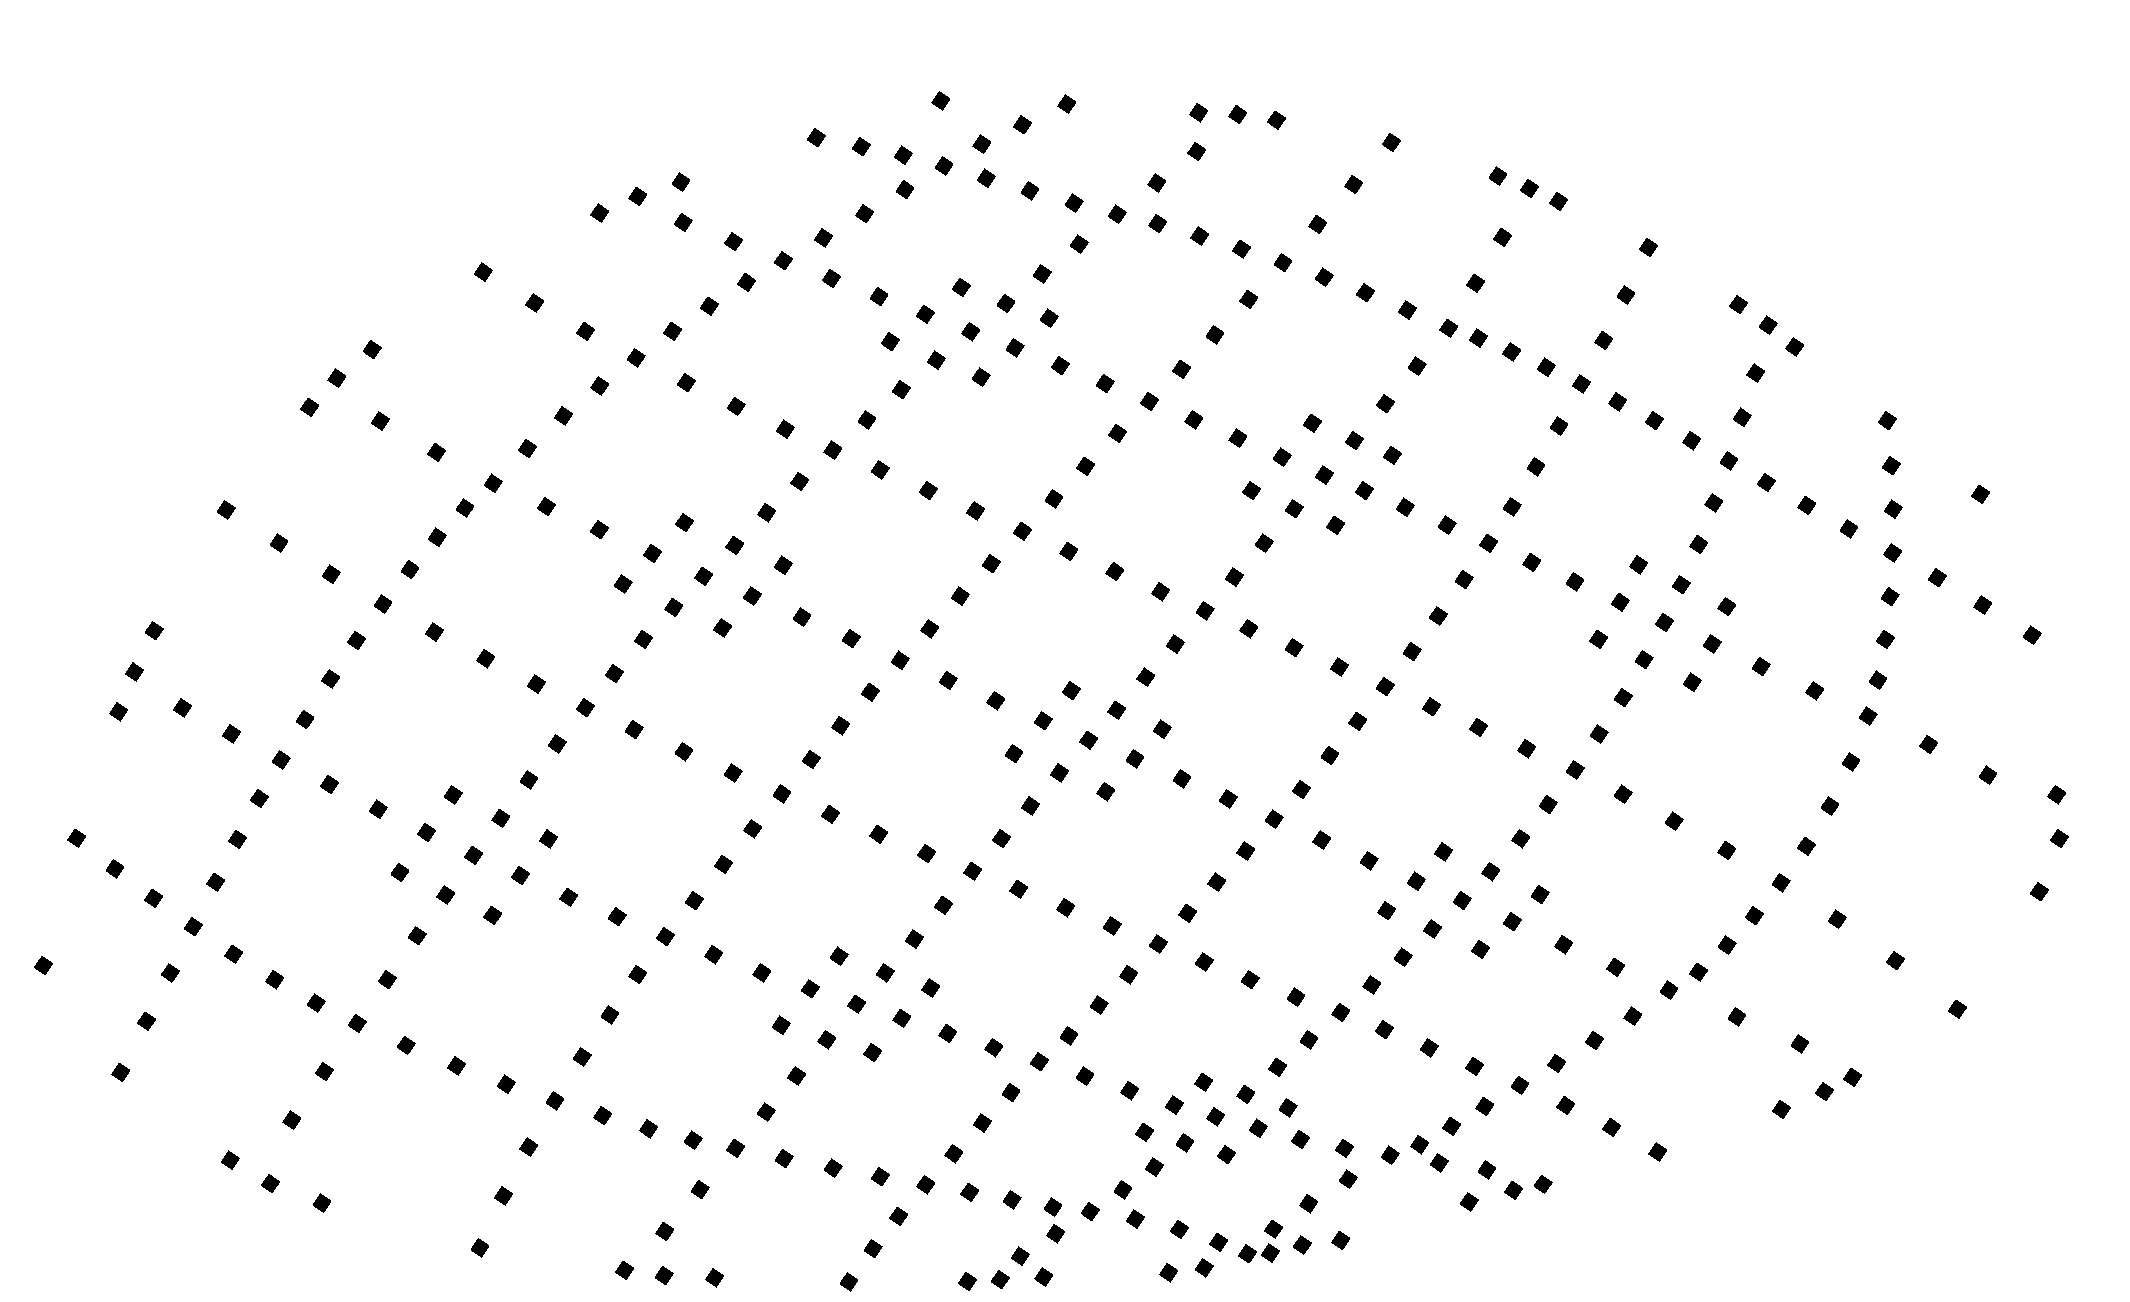
\includegraphics[width=0.5\textwidth]{images/parallel_fiber_estimation/seed_points_level2.png}
  \caption{Parallel mesh generation: Seed points of the streamlines that are traced on processes 0 to 15 in the procedure of \cref{alg:parallel_algorithm_1} at recursion level $l=2$.}
  \label{fig:seed_points_level2}%
\end{figure}

%If more fiber meshes are desired, the 2D elements of this slice can be sampled equidistantly in the parameter space used for the harmonic map computation to obtain more seed points from which additional streamlines are traced.

In summary, the 2D quadrilateral mesh at the center slice of the muscle defines the location of the resulting muscle fibers. Because the construction of this 2D mesh ensured a good mesh quality with similar element sizes, the distance between the resulting fibers is similar and a spatially homogeneous set of muscle fibers is generated.

To obtain the final 1D fiber meshes $\Omega_{F,i}$, the streamlines are sampled at equidistant $z$ intervals, specified by a parameter $\Delta z$. Because the streamlines are directed mainly along the $z$ axis, the constant $z$ interval for the sampling approximately corresponds to the resulting 1D mesh width, i.e., the distance between the points of a fiber. An advantage of this method is that the points of all fibers lie in the same $x$-$y$ planes. Thus, the total set of points can also be interpreted as a structured 3D mesh of the muscle volume $\Omega_M$. This 3D mesh is aligned with the fiber meshes and planes through the $x$ and $y$ axes. These properties are advantageous for data mapping between the 3D mesh and the 1D fiber meshes and for the numerical solution of models with anisotropic advection processes in the 3D mesh that is oriented according to the direction of the fibers.

% file output
At the end, the data is written collectively by all processes into a single file. This is done using the parallel file I/O functionality of MPI. This can be done because the absolute position in the file of every point can be calculated from the index of the point in the structured mesh.

% Examples
\Cref{fig:final_interior_1} gives an example of the resulting streamlines if the recursion ends already after one pass of the procedure at $l_\text{max}=0$. For the example with $l_\text{max}=1$, the selected seed points and the parts of the resulting streamlines in the considered subdomain are shown in \cref{fig:08_final}. Here, the dark blue streamlines on the boundary were traced as part of the refinement actions in line \ref{line:3.6}. Because the recursion ends for $l=1$, these streamlines are now reused for the final fiber meshes instead of further parallel partitioning. Additionally, the light blue streamlines in the interior were traced to obtain a full grid of fibers for the output of the algorithm.

\subsection{Continuation on the Next Recursion Level}

If line \ref{line:3.8} of \cref{alg:parallel_algorithm_1} does not detect the recursion end because the maximum recursion levels is not yet reached, the \code{else} branch in line \ref{line:3.10} is chosen.
Execution continues with the eight times higher number of processes $8^{\ell+1}$. The processes that executed the previous parts of the algorithm send their determined boundaries of the new subdomains to seven other respective processes in line \cref{line:3.11a}. 
Only the first subdomain remains on the same process. Every process stores the boundary points for its new subdomain in the variable \code{boundary\_points}. In line \cref{line:3.11}, the procedure is called recursively and the next recursion level $(l+1)$ begins.

\Cref{fig:06_subdomain} shows the \code{boundary\_points} of the first new subdomain on level $l=2$ for the example on recursion level $l=1$. It consists of the outer boundary (dark yellow lines) and the interior boundary (brown streamlines) and is nearly geometrically similar to the subdomain on level $l=1$. 

\begin{figure}%
  \centering%
  \begin{subfigure}[t]{0.48\textwidth}%
    \centering%
    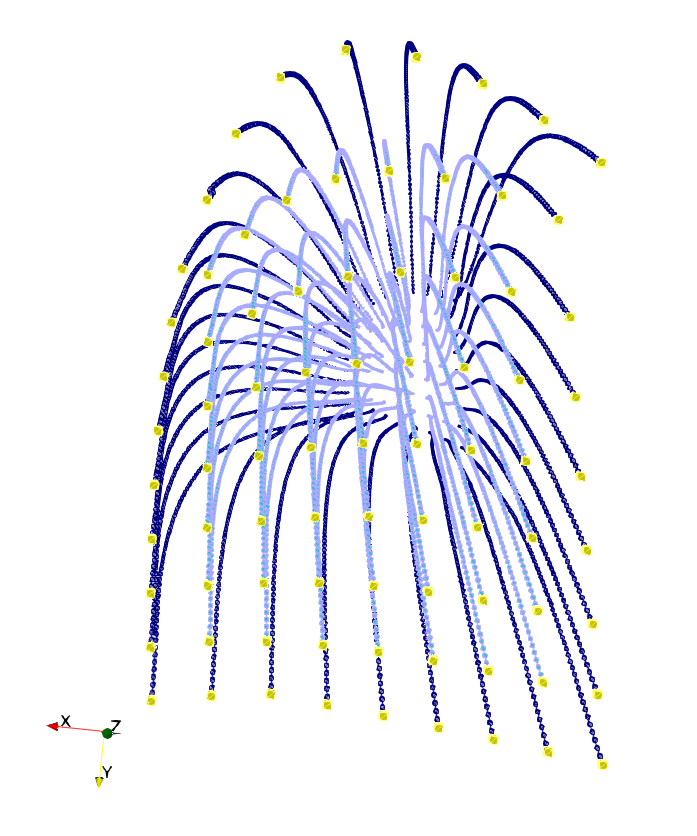
\includegraphics[height=10cm]{images/parallel_fiber_estimation/08_final.png}
    \caption{Seed points (yellow), traced interior streamlines (light blue) and boundary points (dark blue), generated if $l_\text{max}=1$.}%
    \label{fig:08_final}%
  \end{subfigure}
  \quad   
  \begin{subfigure}[t]{0.48\textwidth}%
    \centering%
    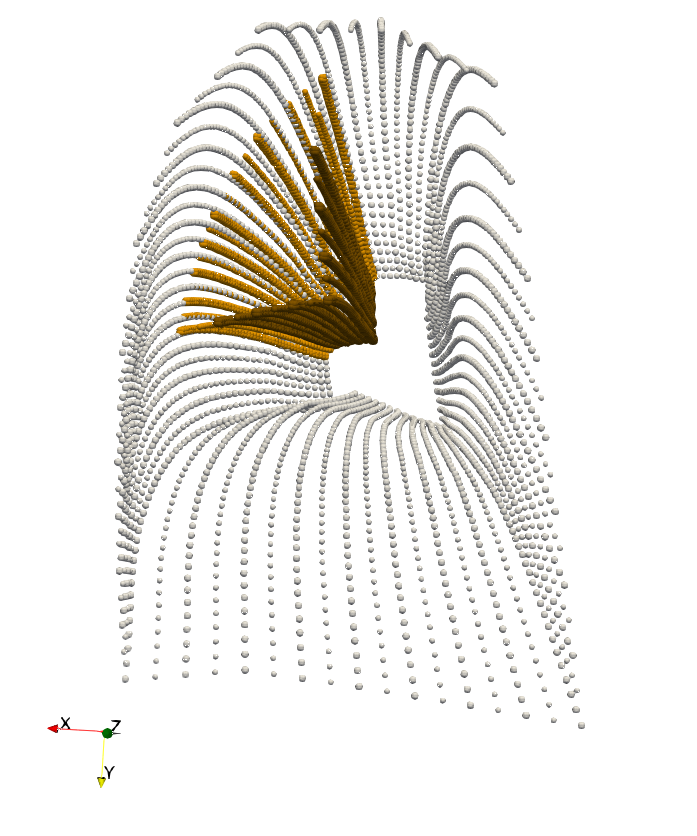
\includegraphics[height=10cm]{images/parallel_fiber_estimation/06_subdomain.png}
    \caption{Boundary points of the first subdomain on level $l=2$ (dark yellow and brown) embedded in the boundary (white) of level $l=1$, generated if $l_\text{max} > 1$.}%
    \label{fig:06_subdomain}%
  \end{subfigure}
   
  \caption{Generation of 3D and 1D meshes in subdomains: Resulting streamlines after the pass of \cref{alg:parallel_algorithm_1} for recursion level $l=1$.}%
  \label{fig:improved}%
\end{figure}%

\subsection{Repair of Incomplete Streamlines}\label{sec:repair_of_incomplete_streamlines}

Practical tests have shown that, for irregular muscle geometries, occasionally some of the streamlines generated in lines \ref{line:3.6} and \ref{line:3.9} of \cref{alg:parallel_algorithm_1} can be incomplete. This means that it was not possible to obtain a streamline that runs through the entire subdomain or the entire muscle domain from top to bottom, instead points are missing for some ranges of $z$ values. This can happen if the streamlines leave the subdomains (because the ghost layer width was chosen too small) or due to numerical errors in irregularly shaped elements mainly on high recursion levels where the system matrix is badly conditioned.

To obtain meaningful results even in these cases, three different repair mechanisms are introduced that interpolate the missing data from valid streamlines. \Cref{fig:fix_invalid} visualizes the cases by examples in a setting of four subdomains with grids of $5 \times 5$ fibers each. The repair mechanisms $\#1$ to $\#3a$ only apply to boundary points. They are executed in line \ref{line:3.6} of the algorithm after the local portions of the streamlines have been traced and before the end points of the streamlines are sent to the neighbor processes below and above that continue the streamline tracing. Mechanismn $\#3b$ and $\#3c$ repair invalid streamlines in the final result and are executed during line \ref{line:3.9} of \cref{alg:parallel_algorithm_1}.

Mechanism \#1 checks all streamlines at subdomain boundaries in the interior, which are shared between neighboring processes. If a streamline is incomplete on one process but complete on the neighbor process, the data of the complete side are transferred such that both processes have the same valid points for this streamline. In the example in \cref{fig:fix_invalid}, the valid streamline data are sent from the top left to the top right subdomain.

Mechanism \#2 checks streamlines at the outer corners of the subdomains. Incomplete streamlines at these locations are recreated from the given boundary points. Because the set of boundary points is twice as coarse as the required number of sample points at these streamlines, every second point gets interpolated from the top and bottom neighbor points.

Mechanism \#3a is concerned with streamlines at interior subdomain boundaries that could not be fixed by mechanism \#1 because the streamlines are incomplete on both sharing processes. In this case, the streamlines are interpolated from the two complete neighboring streamlines that are located next along the boundary as shown in the example in \cref{fig:fix_invalid}. Instead of the factors $\frac13$ and $\frac23$, the actual relation of distances between the seed points of the streamlines is used. The same interpolation is executed independently on both involved processes. Because the valid streamlines have the same data on both subdomains, the resulting fixed streamlines will also be identical.

Mechanisms \#3b and \#3c follow the same approach. They are applied to the interior fibers of the final result and can repair any number of incomplete fibers that are located between complete fibers. This case rarely occurs, a cause can be errors in the numerical solution of the Laplace problem.  In example \#3b in \cref{fig:fix_invalid}, the two invalid streamlines are interpolated from their left and right valid neighbors. In example \#3c, no valid right neighbor exists. Instead, the streamlines are interpolated by using valid positions from the upper and lower neighbors.

\begin{figure}%
  \centering%
  \def\svgwidth{0.8\textwidth}
  \input{images/parallel_fiber_estimation/fix_invalid.pdf_tex}
  \caption{Repair of streamlines used during partitioning and fiber approximation in the 3D and 1D mesh generation: Examples of the four repair mechanisms for estimating incomplete streamlines during the parallel algorithm. Invalid streamlines are indicated by red circles, valid streamlines by black circles. The brown arrows show the direction of data transfer.}%
  \label{fig:fix_invalid}%
\end{figure}%

\subsection{Postprocessing and Output of the Generated Streamlines}\label{sec:postprocessing_of_the_generated_streamlines}

After repairing invalid streamlines, the final result of the algorithm is a grid with $(2\,n_\text{el,x}\,n_x+1) \times (2\,n_\text{el,x}\,n_x+1)$ fibers in the $x$-$y$ plane and a configurable number of points in $z$ direction, where $n_x = 2^{\ell_\text{max}}$ is the number of subdomains per coordinate direction on the last recursion level. 

If a higher number of fibers is desired than is naturally generated by the parallel algorithm, additional fibers can be created by interpolation in the existing grid of fibers, which is parallel partitioned. The implementation of the presented algorithm in \opendihu{} includes this postprocessing functionality as part of the mesh generation program. Alternatively, the step can be applied separately on any binary output file that contains a grid of fibers. 

The action of increasing the number of fibers proceeds as follows. The initial grid contains the fibers that were created from the streamlines, called \emph{key fibers}.
A specified number $m$ of additional fibers is placed between the key fibers in both $x$ and $y$ coordinate directions.
The additional fibers together with the key fibers form a grid of fibers in the muscle cross sections with an $m$ times finer mesh width. In the grid of key fibers, every portion bounded by $2 \times 2$ key fibers contains $(2+m)^2 - 4$ additional fine fibers. The total number of fibers depending on $n_x$ and $m$, therefore, is $N=(2\,n_\text{el,x}\,n_x\,(1+m)+1)^2$. Due to construction, this number is always odd. This is a desired property because it yields an even number of elements per coordinate direction and this allows to construct a mesh with quadratic ansatz functions.

The new fibers are computed by barycentric interpolation. The location of every new point $\bfp$ is calculated from the nearest points $\bfp_0, \bfp_1, \bfp_2$ and $\bfp_3$ of key fibers in the $x$-$y$ plane, numbered according to  \cref{fig:quads_tris}, by%
\begin{align}\label{eq:mesh_barycentric_interpolation}
  \bfp = (1-\alpha_x)\,(1-\alpha_y)\,\bfp_0 + \alpha_x\,(1-\alpha_y)\,\bfp_1 
        + (1-\alpha_x)\,\alpha_y\,\bfp_2 + \alpha_x\,\alpha_y\,\bfp_3.
\end{align}
Here, the factors $\alpha_x,\alpha_y \in [0,1]$ are chosen in a way to create the fine grid of fibers:
%
\begin{align*}
  \alpha_x = i / (m+1), \quad \alpha_y = j / (m+1)\quad \text{ for }i,j = 0, \dots,m, \quad (i,j) \neq (0,0).
\end{align*}
As a result, we can generate a 3D mesh where the number of points in $x$ and $y$ directions can be adjusted by the parameter $m$. 

An advantage of this algorithm is that each process only has to keep the data of its own subdomain in memory at any time. This allows parallel processing of very large meshes. For small-enough meshes that do not fall under this restriction, the utility script \code{resample_bin_fibers.py} can be used to create meshes of any resolution from any other mesh using the barycentric interpolation in \cref{eq:mesh_barycentric_interpolation}. An example is given in \cref{fig:left_biceps_brachii_33x33fibers_refined}, where a mesh of  $33\times 33$ fibers is refined by interpolation to a mesh with $71\times 71$ fibers.

% seed points 33x33, 71x71 from scaling script
\begin{figure}[H]
  \centering%
  \begin{subfigure}[t]{0.48\textwidth}%
    \centering%
    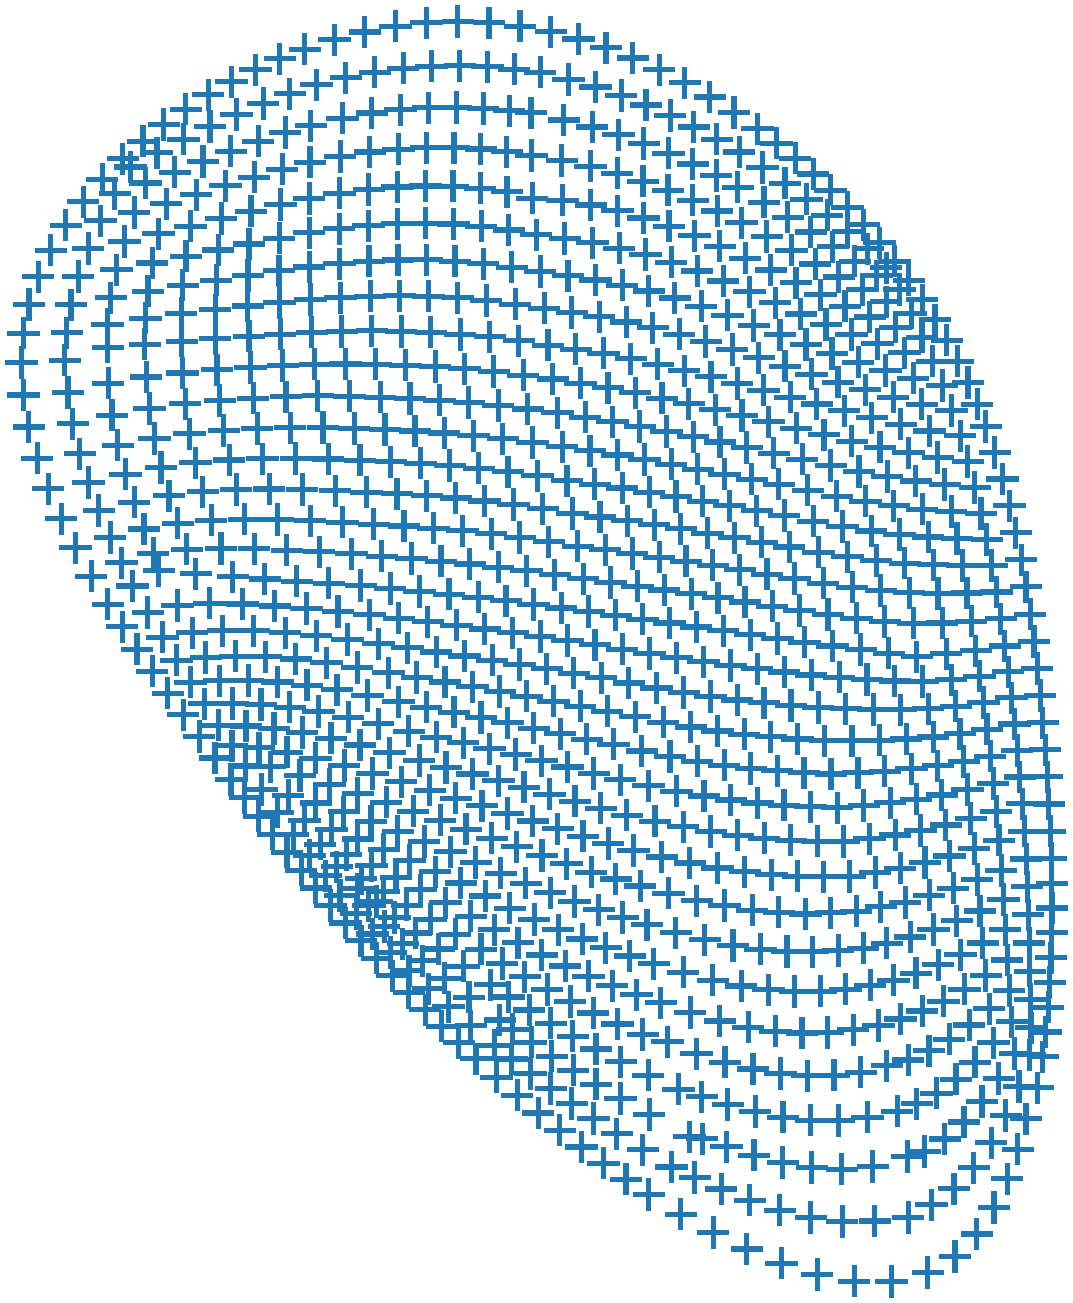
\includegraphics[width=\textwidth]{images/parallel_fiber_estimation/left_biceps_brachii_33x33fibers_bin_csv.pdf}%
    \caption{Mesh points in a $33\times 33$ grid at the center cross section of the biceps muscle.}%
    \label{fig:left_biceps_brachii_33x33fibers_bin_csv}%
  \end{subfigure}
  \quad
  \begin{subfigure}[t]{0.48\textwidth}%
    \centering%
    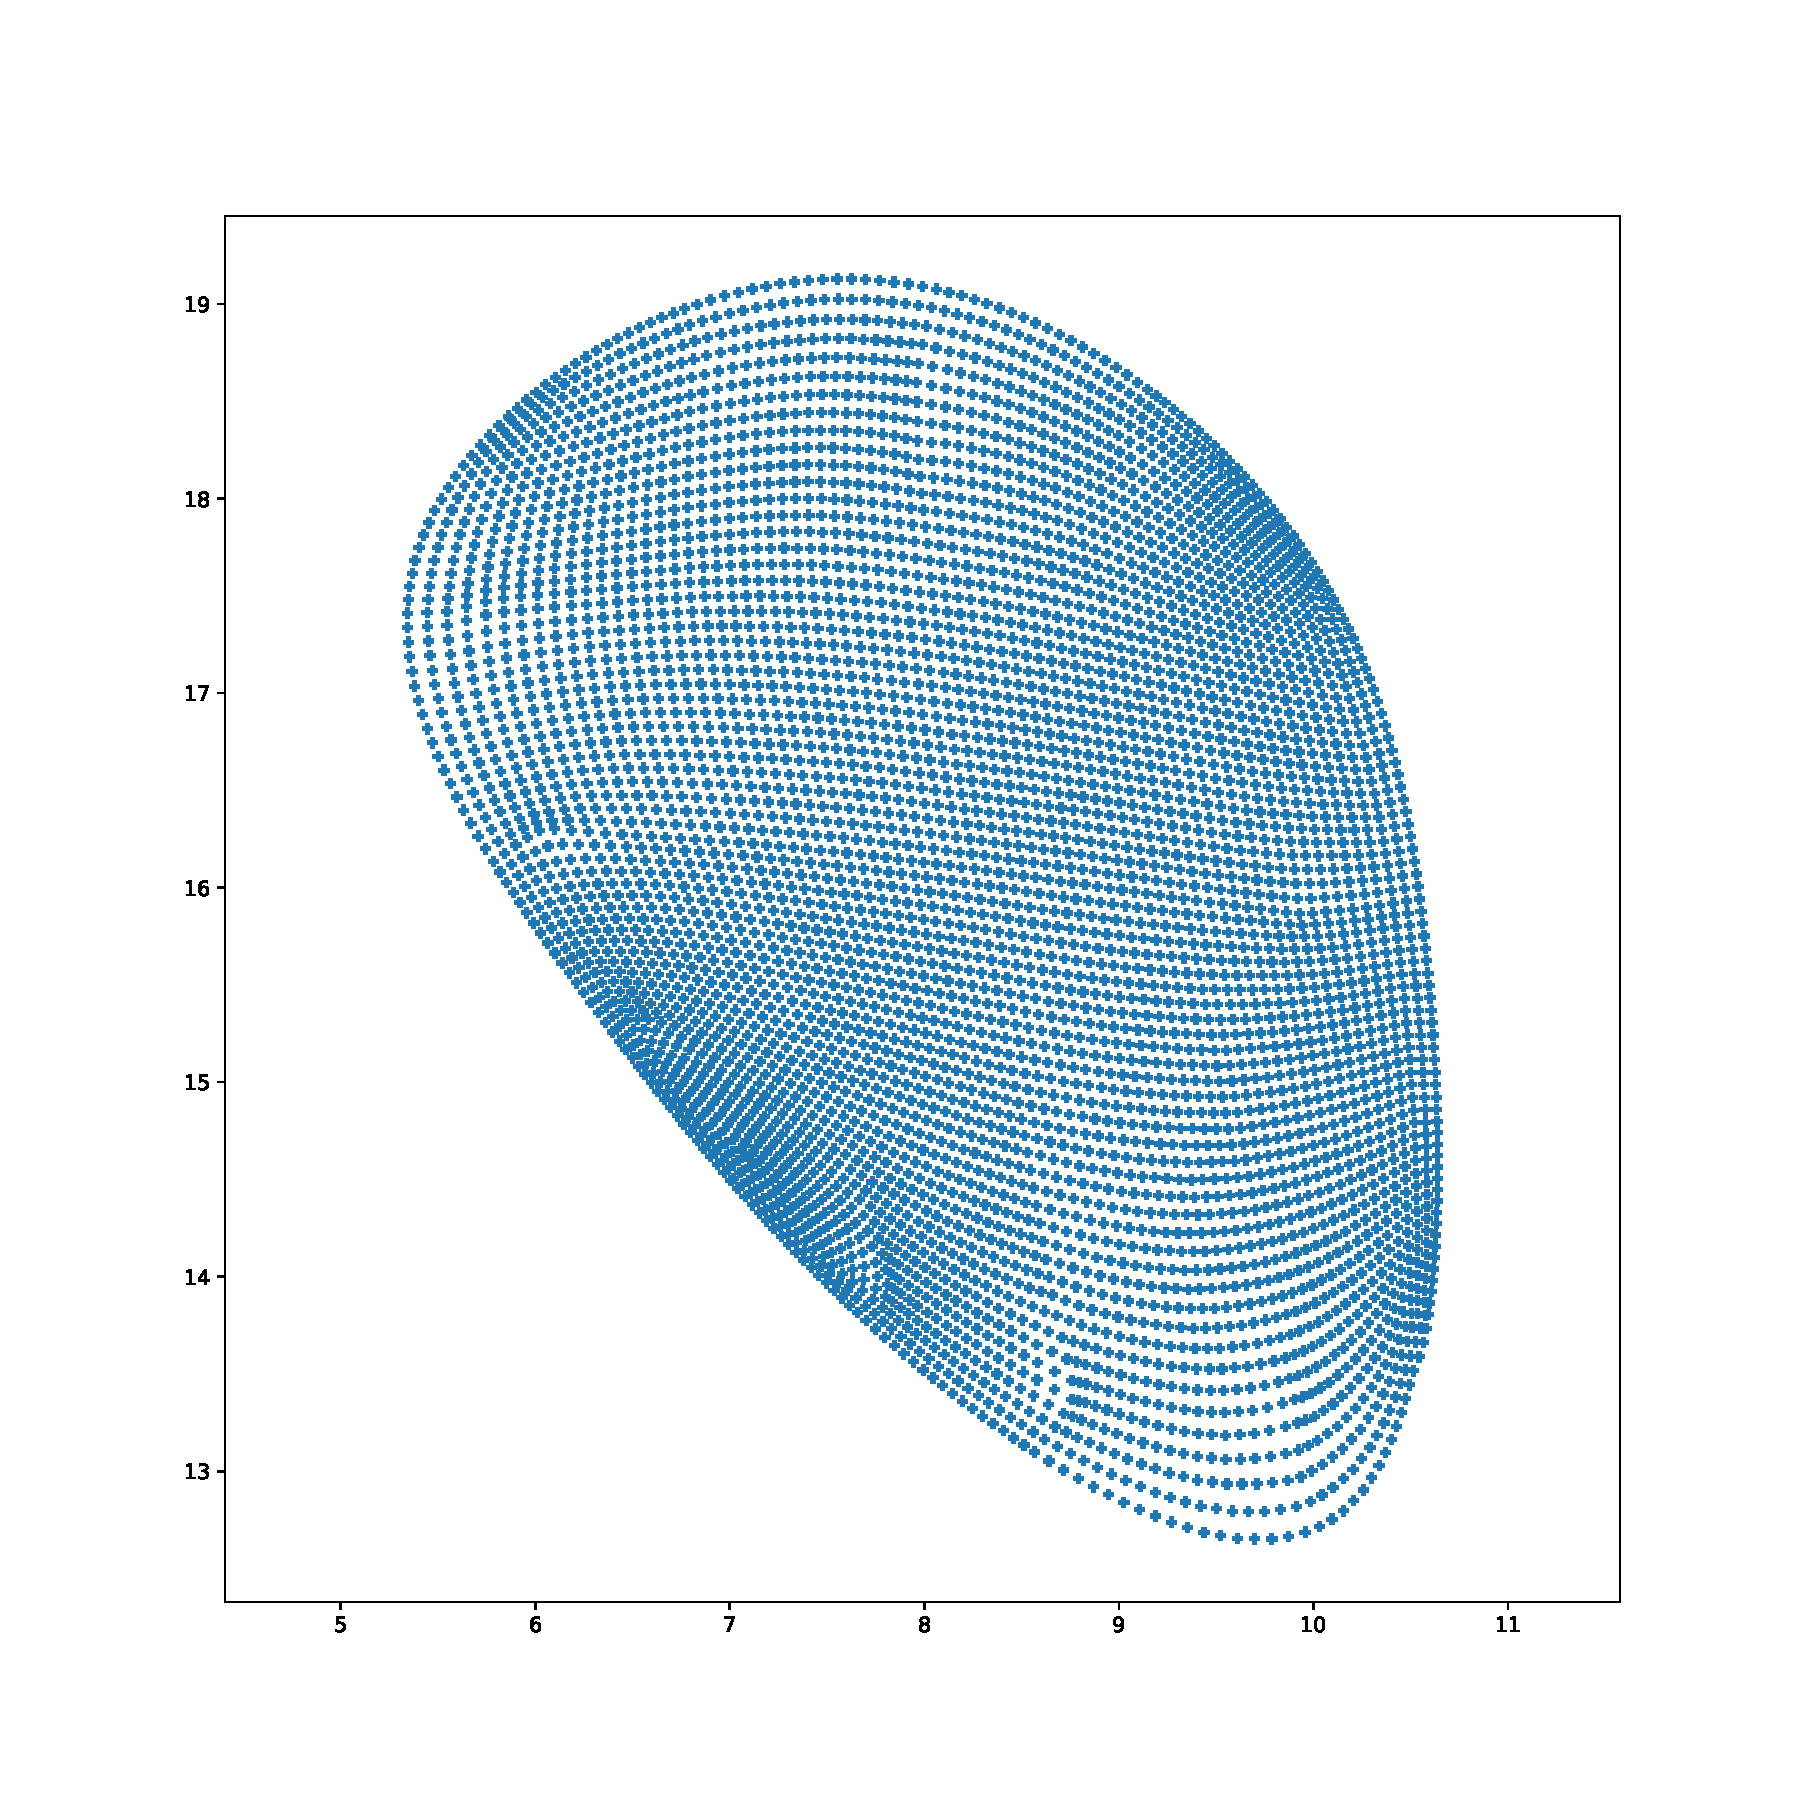
\includegraphics[width=\textwidth]{images/parallel_fiber_estimation/left_biceps_brachii_71x71fibers_bin_csv.pdf} % also png
    \caption{Refined mesh points in a $71\times 71$ grid that were obtained from (a) by barycentric interpolation.}%
    \label{fig:left_biceps_brachii_71x71fibers_bin_csv}%
  \end{subfigure}   
  \caption{Refinement of existing meshes to obtain derived meshes with any number of nodes.}%
  \label{fig:left_biceps_brachii_33x33fibers_refined}%
\end{figure}%


The resulting points are stored in a binary file format. The contents of this output file can either be interpreted as grid points of a 3D mesh or as points of individual 1D fibers. This is an advantage in a multi-scale simulation where both a 3D muscle mesh and multiple embedded 1D fiber meshes occur: First, all mesh information of both $\Omega_M$ and $\Omega_{F,i}$ can be given by a single file. And second, the 3D mesh is aligned with the 1D fibers and all 3D mesh points are also 1D mesh points. 

The spacing in $z$ direction between points on a fiber is typically chosen as $\Delta z = \SI{0.01}{\cm}$. This value was found to ensure a low error in the model for propagation of electric stimuli along the muscle. The value leads to 1481 points per fiber on the belly of the biceps muscle. 

Every point coordinate is stored in the output file as double precision value with eight bytes. The file contains a header of 72 bytes with descriptive information such as the number of fibers, some parameter values and a time stamp. The total file size therefore can be calculated by $72+N\cdot 1481\cdot 3\cdot 8$ bytes.

Often, the spatial resolution of the 3D mesh does not need to be as high as those of the fibers. The relation of the 3D and 1D mesh widths as well as the number of 1D meshes should be choosen such that the numerical error of the simulation in both domains is balanced.
In case the 3D mesh should be coarser than the output of the algorithm, we can use only a subset of the points contained in the output file. Then, a stride in $x$, $y$, and $z$ direction is specified in the settings for the simulation. The corresponding coarse grid of points is extracted and used to construct the 3D mesh that is then used for the simulation.
%The 1D fiber meshes use all given points in the file.
% When a 3D mesh with a smaller spatial resolution in $x$ and $y$ direction than the number of fibers is used in a simulation together with 1D fiber meshes from the same file, some of the fibers at the outer layer can be located outside of the 3D mesh. A way to avoid this is to not use the outer layer of fibers. 


A remaining issue concerns the mesh quality on the outer boundary. In general, the 3D mesh created by \cref{alg:parallel_algorithm_1} has good quality because the interior points result from smooth streamlines that were traced through a divergence free vector field. 
The points at the boundary, however, are either sampled from a triangulation of a tubular surface of the muscle or computed from the NURBS formulation. This surface is derived from imaging data, as described in \cref{sec:preprocessing_of_the_muscle_geometry}. If the triangulation is used, the quality of the boundary points of the created mesh depends on the quality of the muscle surface and its triangulation. In a case where this quality is poor, only the outer layer of elements of the created 3D mesh is affected. \Cref{fig:poor_boundary_33x33} shows an example for this effect in a grid of $9 \times 9$ fibers. It can be seen that only the fibers at the bottom of the image have an irregularity at their center. Such an irregularity potentially occurs at every $z$ coordinates where a new subdomain begins. The cause is that, at these locations, the points on the rings are slightly shifted relative to each other.

A remedy in such a case is to discard the outer layer of fibers and construct the mesh only from points of the inner streamlines.
Accordingly, our implementation of the presented algorithm \cref{alg:parallel_algorithm_1} always creates two different output files. The first output file contains all fibers, the second contains all except the outer layer of fibers. The second file contains only $N=(2\,n_\text{el,x}\,n_x\,(1+m)-1)^2$ instead of $N=(2\,n_\text{el,x}\,n_x\,(1+m)+1)^2$ fibers.
\begin{figure}%
  \centering%
  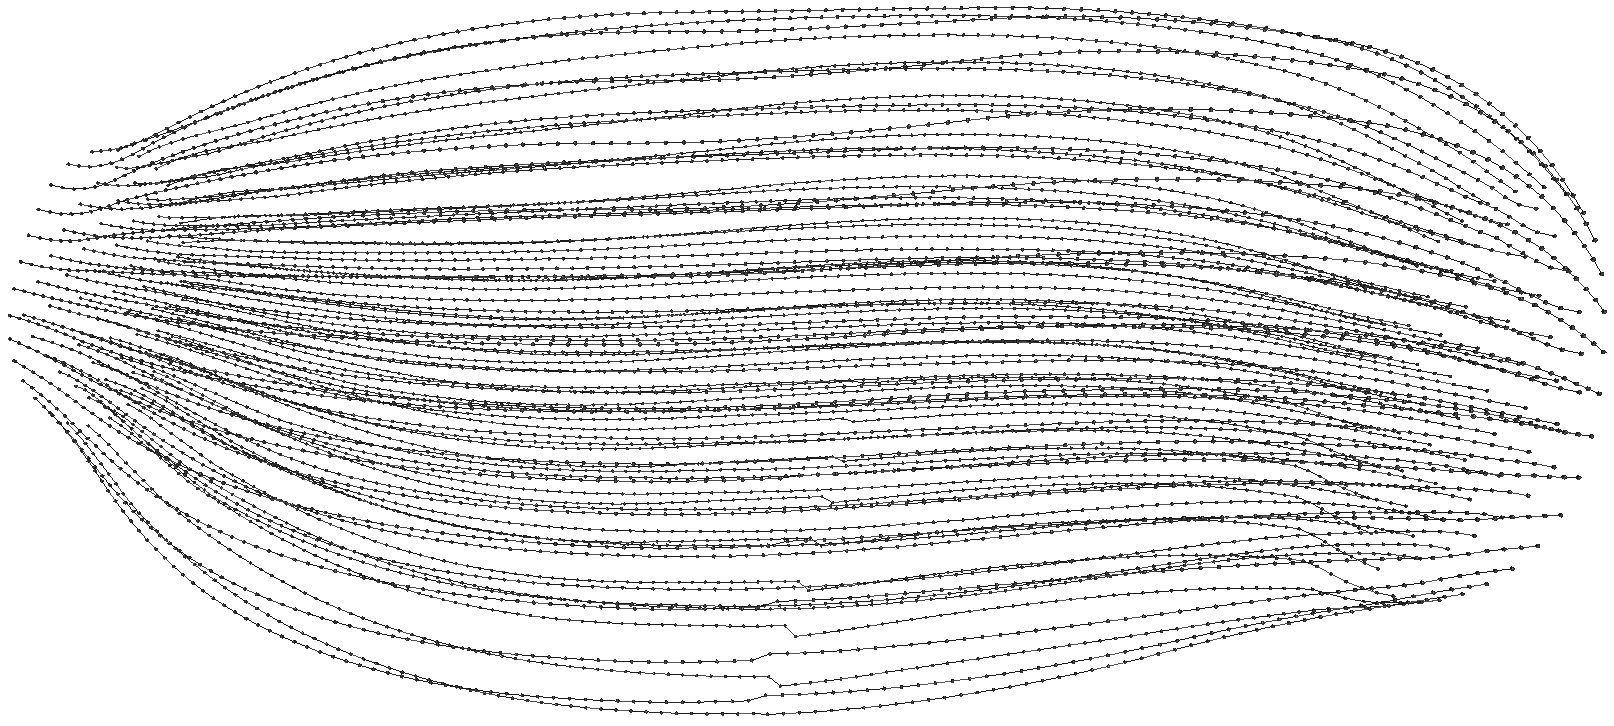
\includegraphics[width=\textwidth]{images/parallel_fiber_estimation/poor_boundary_33x33.png}%
  \caption{Evaluation of the parallel mesh generation algorithm, \cref{alg:parallel_algorithm_1}: Resulting fibers and points on the fibers created with the parallel algorithm, $9\times 9$ fibers with $1481$ nodes each. Irregularities in the outer surface can be seen in the  center at the bottom of the image.}%
  \label{fig:poor_boundary_33x33}%
\end{figure}%

\section{Results and Discussion}

The following section presents results of the parallel algorithm for mesh generation, \cref{alg:parallel_algorithm_1}. In addition, the effect of various parameters is investigated.

Two types of parameters can be distinguished. Parameters of the first type influences the number of nodes in the resulting mesh. These parameters have to be set such that the desired mesh resolution is achieved. Often, multiple, different parameter combinations are possible to achieve a given mesh resolution.
Parameters of the second type have no effect on the mesh resolution but on the quality of the mesh. Usually, the parameter combination that gives the highest mesh quality should be chosen.

In the following, \cref{sec:mesh_generation_resulting_meshes} shows results of the algorithm. Then, \cref{sec:mesh_generation_mesh_size_parameters} outlines how parameters of the first type affect the mesh resolution. A specific parameter, the recursion width, is discussed in \cref{sec:mesh_generation_recursion_width}. Subsequently, \cref{sec:mesh_generation_mesh_quality_parameters} evaluates and discusses parameters of the second type, which affect the mesh quality.

\subsection{Resulting Meshes}\label{sec:mesh_generation_resulting_meshes}

At first, results of the whole workflow described in \cref{sec:overview_and_notation_of_required_meshes} to \cref{sec:parallel_algorithm} are presented.
The input for the mesh generation algorithm is a geometry representation, which is typically extracted from biomedical imaging. The output of the parallel algorithm, \cref{alg:parallel_algorithm_1}, comprises a 3D mesh with hexahedral elements as well as multiple, embedded 1D fiber meshes. 

\Cref{fig:muscle_meshes} visualizes some results for the biceps and triceps muscles.
The parameter values $n_\text{el,x}=4$, $n_\text{el,z}=50$ and $m=0$ are chosen. If the recursion level is set to $l_\text{max}=0$, the algorithm generates meshes with the smallest possible number of fibers, which is a grid of $7 \times 7$ fibers.  
\Cref{fig:muscle_mesh_0} shows a grid of $7\times 7$ fibers and the corresponding 3D mesh that was sampled from the fiber data using every 50th point in $z$ direction of the fiber meshes. It can be seen that the generated fibers traverse all nodes of the generated 3D mesh and, thus, the 3D mesh is aligned with the fiber direction.

\Cref{fig:muscle_mesh_1} shows a similar result with $9 \times 9$ fibers. Here, the colors correspond to the solution of an electrophysiology simulation. Blue regions indicate that the fiber membranes have an electric potential equal to their resting potential, which indicates no activation. Orange and red colors correspond to activated regions. It can be seen that the activation is present at the same locations on both the fibers and the 3D mesh. In the simulation, this requires data mapping from the fiber meshes to the 3D mesh. Because all nodes of the 3D mesh are located on the fibers, this data transfer becomes trivial.

\Cref{fig:muscle_mesh_2,fig:muscle_mesh_3} present grids with $13 \times 13$ and $67 \times 67$ fibers of the biceps muscle, respectively. Results with larger numbers of fibers are not shown here because in such visualizations the fibers become less distinguishable. \Cref{fig:muscle_mesh_4,fig:muscle_mesh_5} show fibers for the triceps geometry.

\begin{figure}%
  \centering%
  \begin{subfigure}[t]{0.30\textwidth}%
    \centering%
    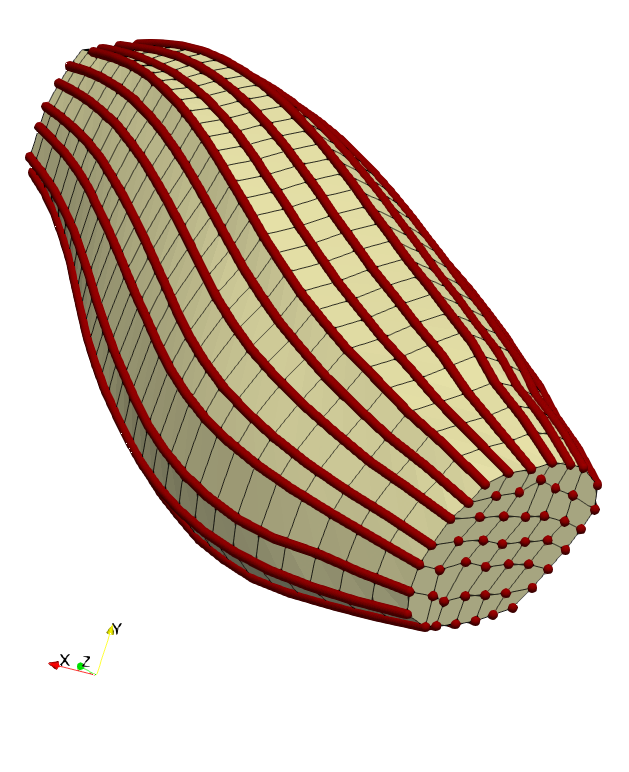
\includegraphics[height=7cm]{images/parallel_fiber_estimation/muscle_mesh.png}
    \caption{Grid of $7 \times 7$ fibers (red) and the aligned 3D mesh with $7 \times 7 \times 30$ nodes (yellow).}%
    \label{fig:muscle_mesh_0}%
  \end{subfigure}
  \quad
  \begin{subfigure}[t]{0.30\textwidth}%
    \centering%
    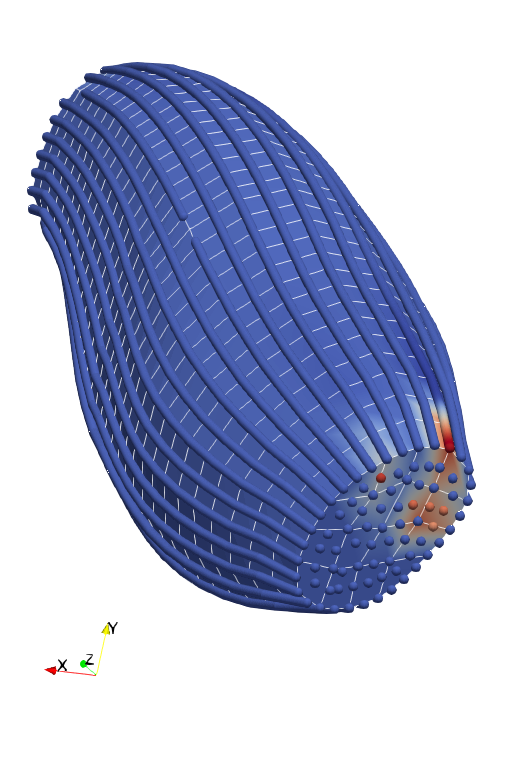
\includegraphics[height=7cm]{images/parallel_fiber_estimation/muscle_mesh_1b.png}
    \caption{Grid of $9 \times 9$ fibers and 3D mesh with the solution of an electrophysiology simulation.}%
    \label{fig:muscle_mesh_1}%
  \end{subfigure}  
  \quad 
  \begin{subfigure}[t]{0.30\textwidth}%
    \centering%
    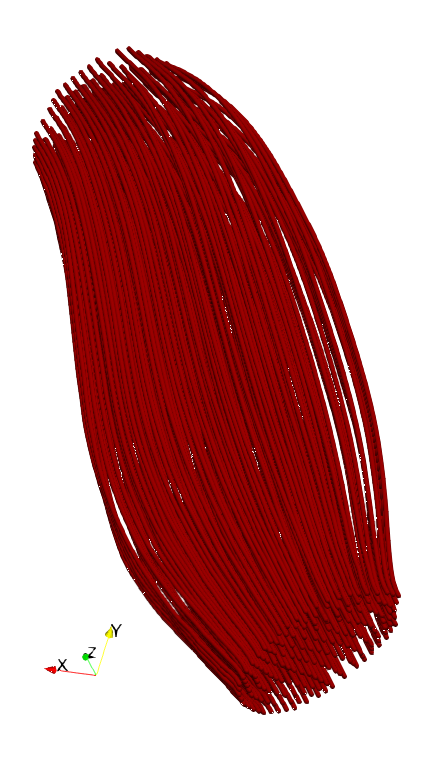
\includegraphics[height=7cm]{images/parallel_fiber_estimation/muscle_mesh_2b.png}
    \caption{Grid of $13 \times 13$ fibers.}%
    \label{fig:muscle_mesh_2}%
  \end{subfigure}
  \\
  \begin{subfigure}[t]{0.25\textwidth}%
    \centering%
    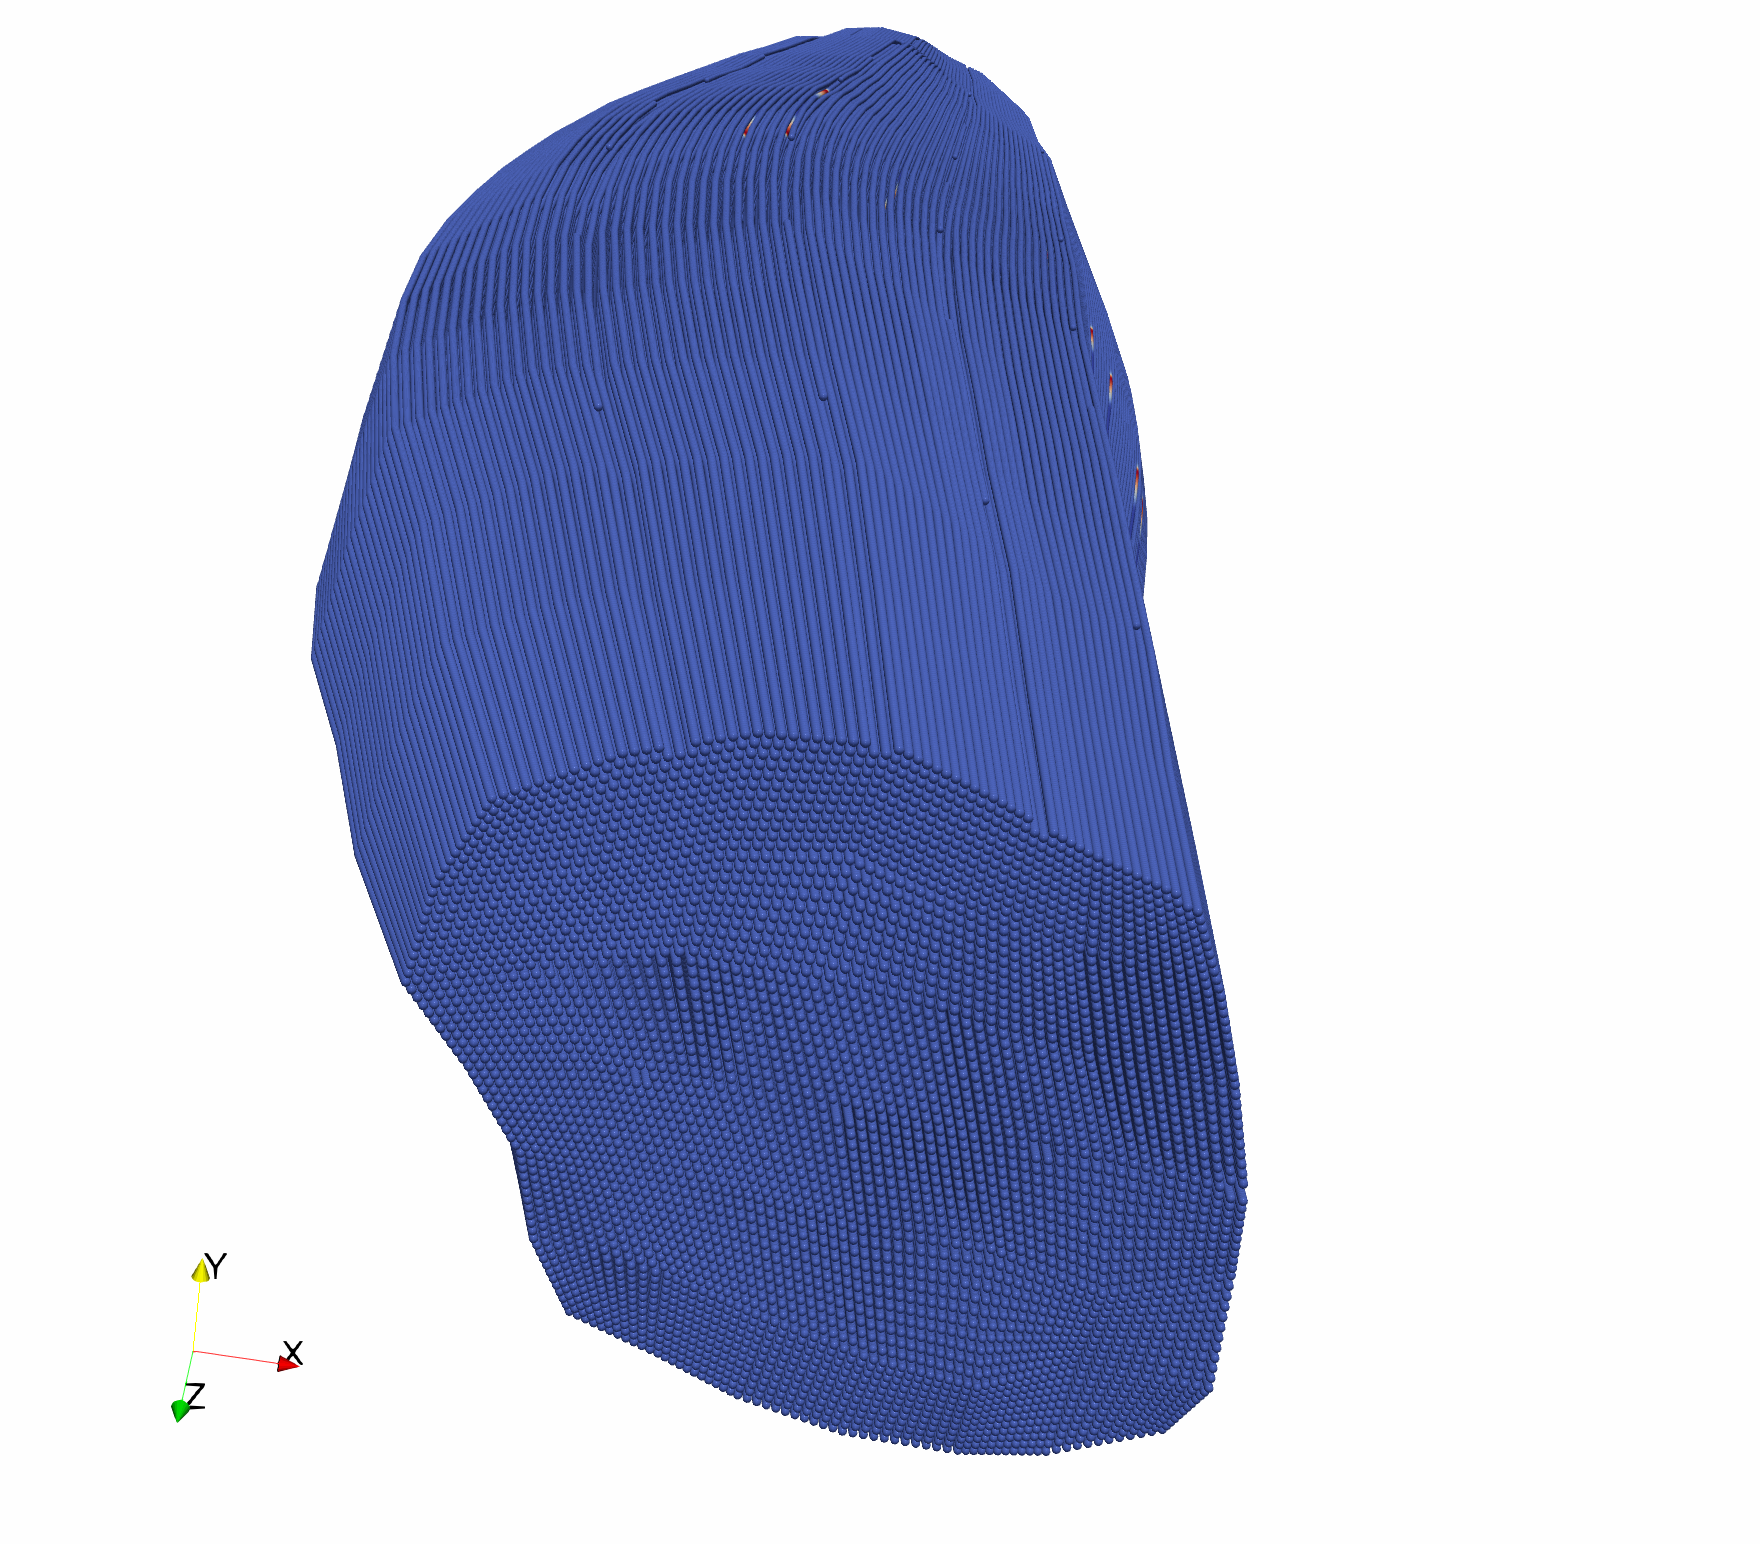
\includegraphics[height=5cm]{images/parallel_fiber_estimation/muscle_mesh_3.png}
    \caption{Grid $67 \times 67$ muscle fibers for the biceps geometry}%
    \label{fig:muscle_mesh_3}%
  \end{subfigure} 
  \,
  \begin{subfigure}[t]{0.15\textwidth}%
    \centering%
    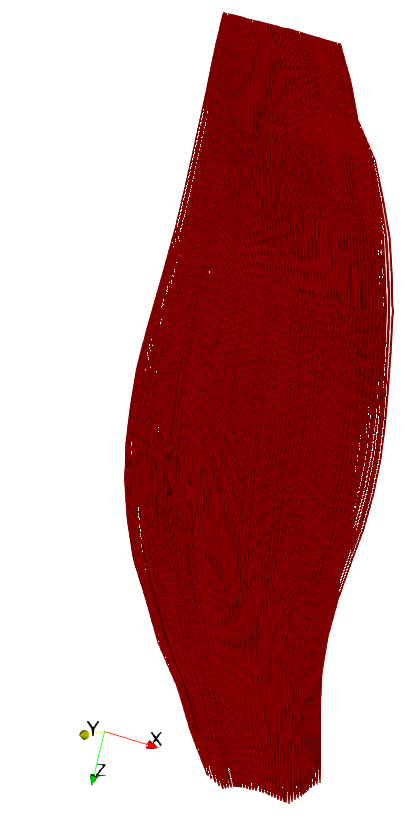
\includegraphics[height=5cm]{images/parallel_fiber_estimation/triceps_25x25.png}
    \caption{$25 \times 25$ fibers of triceps}%
    \label{fig:muscle_mesh_5}%
  \end{subfigure} 
  \hfill
  \begin{subfigure}[t]{0.55\textwidth}%
    \centering%
    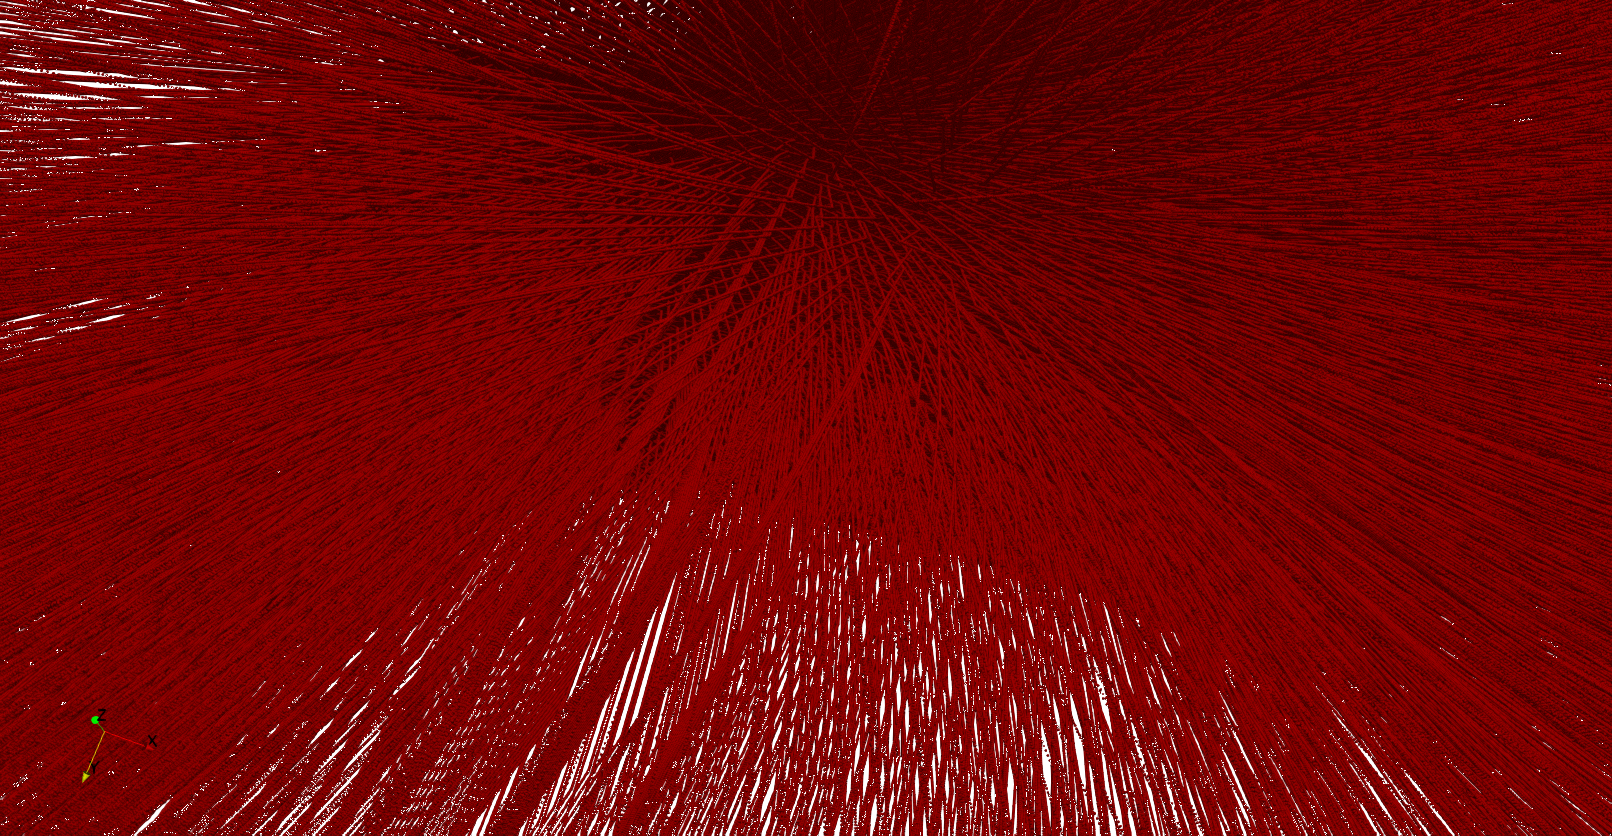
\includegraphics[width=\textwidth]{images/parallel_fiber_estimation/triceps_inside_67x67c.png}
    \caption{Grid of $67 \times 67$ fibers for the triceps geometry as seen from within the muscle. The total number of points is \num{8982489}.}%
    \label{fig:muscle_mesh_4}%
  \end{subfigure}  
   
  \caption{Evaluation of the parallel mesh generation algorithm, \cref{alg:parallel_algorithm_1}: 1D fiber meshes and corresponding 3D meshes. The biceps geometry is used in (a)-(d), the triceps geometry in (e) and (f). The fibers have 1481 nodes each in the biceps muscle and 2001 nodes each in the triceps muscle.}%
  \label{fig:muscle_meshes}%
\end{figure}%

\subsection{Effect of Mesh Size Parameters}\label{sec:mesh_generation_mesh_size_parameters}

Next, the type of parameters that affect the resulting mesh resolution is discussed.
The choices of the maximum recursion level $\ell_\text{max}$, the number $n_\text{el,x}$ of elements in $x$ direction of the subdomains and the fine grid parameter $m$ determine the resulting number $N$ of fibers and, thus, the file size of the binary output file. The formulas for these numbers were given in \cref{sec:postprocessing_of_the_generated_streamlines}. \Cref{tab:file_sizes} lists exemplary numbers of fibers and file sizes for $n_\text{el,x}=4$ and different values of $\ell_\text{max}$ and $m$. The number $n_\text{proc}$ of required processes to reach the maximum recursion level is also listed, it depends on $\ell_\text{max}$ by $n_\text{proc}=8^{\ell_\text{max}}$.

Two different numbers of fibers and corresponding file sizes are listed for every parameter combination. The two variants correspond to the two files that include respectively omit the fibers at the boundary.

The table shows that meshes with different sizes can be constructed by appropriate choices of parameters. A realistic biceps muscle contains about \num{200000} to \num{400000} muscle fibers \cite{MacDougall1984}. The table shows that constructing a mesh in this range yields a file with a size of $\approx$\SI{10}{\gibi\byte}.\footnote{
In this work, file sizes are given using multiples of bytes (B) and the prefixes defined in the ISO/IEC International System of Quantities \cite{ISOmebi}. The prefixes are: 1 kibibyte (\SI{1}{\kibi\byte})=$2^{10}$ bytes, 1 mebibyte (\SI{1}{\mebi\byte})=$2^{20}$ bytes, 1 gibibyte (\SI{1}{\gibi\byte})=$2^{30}$ bytes}
A mesh that contains \SI{1}{\percent} of the realistic number of fibers can be stored in a file with size of $\approx$\SI{100}{\mebi\byte}.

The binary files to store the generated meshes are small compared to ASCII-based file formats as each point coordinate is represented by only eight bytes. For comparison, the ASCII-based \emph{exnode} format defined within the OpenCMISS framework uses 24 characters, i.e., 24 bytes to store one point coordinate. Additionally, a larger memory overhead for the description of the data is needed such that \emph{exnode} files are more than three times larger than the binary files used in \opendihu{}.

The binary file format uses no compression that could further reduce the file size. The reason is that no extra effort should be needed when writing programs that parse these files. Thus, they can easily be handled by codes in different programming languages. For example, within \opendihu{} the file format is understood by various Python scripts and C++ programs.

\begin{table}
  \centering%
  \begin{tabular}{|l|l|l| r@{\,=\,}l r|rr|}
    \hline
    max.                      &fine grid     &\# proc. &  \multicolumn{2}{c}{\begin{tabular}{lrr} \# fibers && \end{tabular}}&file size \\
    level $\ell_\text{max}$   & $m$          & $n_\text{proc}$         & \multicolumn{2}{c}{\begin{tabular}{lll} &&\end{tabular}}&\\
    \hline
    0     & 0      & 1     & $9\times 9$      & \num{81} & \SI{2.7}{\mebi\byte} \\
          &        &       & $7\times 7$      & \num{49} & \SI{1.7}{\mebi\byte}\\
    0/1   & 1/0    & 1/8   & $17\times 17$    & \num{289} & \SI{9.8}{\mebi\byte}\\
          &        &       & $15\times 15$    & \num{225} & \SI{7.6}{\mebi\byte}\\
    0/1/2 & 3/1/0  & 1/8/64 & $33\times 33$    & \num{1089} & \SI{36.9}{\mebi\byte}\\
          &        &       & $31\times 31$    & \num{961} & \SI{32.6}{\mebi\byte}\\\hline
    0     & 7      & 1     & $65\times 65$    & \num{4225} & \SI{143.2}{\mebi\byte}\\
          &        &       & $63\times 63$    & \num{3969} & \SI{134.5}{\mebi\byte}\\
    2     & 7      & 64     & $257 \times 257$ & \num{66049} & \SI{2.2}{\gibi\byte}\\
          &        &       & $255 \times 255$ & \num{65025} & \SI{2.2}{\gibi\byte}\\
    2     & 15     & 64    & $513 \times 513$ & \num{263169} & \SI{8.7}{\gibi\byte}\\
          &        &       & $511 \times 511$ & \num{261121} & \SI{8.6}{\gibi\byte}\\
    \hline
  \end{tabular}
  \caption{Parallel 1D and 3D mesh generation: Different parameter choices of $l_\text{max}$ and $m$ and the resulting number $n_\text{proc}$ of processes, number of fibers and file size. Some results can be achieved with different parameter combinations, e.g., both $\ell_\text{max}=0, m=1$ and $\ell_\text{max}=1, m=0$ result in $17\times 17$ fibers. These combinations are separated by slashes.}%
  \label{tab:file_sizes}%
\end{table}

\subsection{Effect of the Recursion Width}\label{sec:mesh_generation_recursion_width}

Some numbers of fibers can be achieved with multiple, different parametrizations that use different recursion widths. \Cref{tab:file_sizes} contains such alternatives for $\ell_\text{max}$ and $m$ separated by slashes in the second and third row. For example, the three combinations $(\ell_\text{max} = 0, m=3)$, $(\ell_\text{max} = 1, m=1)$, and $(\ell_\text{max} = 2, m=0)$ all lead to a grid of $31 \times 31$ fibers (without boundary layer). However, the spatial location of the fibers in the muscle is not identical for these alternatives, because the intermediate mesh used for the streamline tracing of the fibers is differently resolved.
In the case with recursion depth $\ell_\text{max} = 0$ and fine grid interpolation parameter $m=3$, numerous of the resulting fibers are interpolated from a coarse grid whereas in the case with $\ell_\text{max} = 2$ and $m=0$ all fibers are key fibers and are obtained by streamlines tracing through a fine mesh.

\Cref{fig:different_recursion_levels} shows parts of the resulting meshes at the longitudinal center of the muscle for these two cases.
In \cref{fig:31x31_l0_center}, the mesh obtained with $l_\text{max}=0$ consists of a grid of traced key fibers and an interpolated finer grid of fibers. The key fiber grid  is given by the corners of the gray checkerboard pattern in the image. It can be seen that the mesh consists of patches with $4 \times 5$ or $5 \times 5$ fibers that each have equal element lengths and angles. In comparison, the mesh in \cref{fig:31x31_l2_center} that was obtained with $l_\text{max}=2$ consists only of key fibers. Here, the change in shape going from one element to its neighbors occurs more smoothly than in \cref{fig:31x31_l0_center}. This qualitatively implies a higher mesh quality.

To quantify this effect, we introduce a measure for mesh quality and compare the scores of the three alternatives in the present example. We consider all angles that occur in an element in the $x$-$y$ plane. The mean value of all angles is obviously $\pi/2$. The variance of all angles can be used as the measure for mesh quality. If the variance is low, this indicates similar elements and, thus, good mesh quality. 

For the present example, the variance was computed for the mesh with $31 \times 31$ fibers and \num{1481} nodes per fiber and, thus, $\num{1332000}$ 3D elements in total.
\Cref{fig:2mesh_quality} plots the variance for the three cases given in the third row of \cref{tab:file_sizes}, i.e., parameter combinations $(l_\text{max}=0,m=3)$, $(l_\text{max}=1,m=1)$ and $(l_\text{max}=2,m=0)$. The 3D mesh corresponding to the lowest bar contains the 2D mesh shown in \cref{fig:31x31_l0_center} and the 3D mesh corresponding to the upper-most bar contains \cref{fig:31x31_l2_center}. 

It can be seen that the quality of meshes on higher recursion levels with less interpolation increases as expected.
This emphasizes the benefit of the parallel algorithm that uses finer meshes compared to the mesh used during serial execution of the algorithm.

\begin{figure}%
  \centering%
  \begin{subfigure}[t]{0.45\textwidth}%
    \centering%
    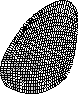
\includegraphics[width=0.9\textwidth,trim=0 0 8mm 1cm, clip]{images/parallel_fiber_estimation/31x31fibers_l0_m3_2In_dirichlet.pdf}
    \caption{Result for parameters $l_\text{max}=0, m=3$, i.e., with three interpolated fibers between every two traced fibers.}%
    \label{fig:31x31_l0_center}%
  \end{subfigure}
  \quad
  \begin{subfigure}[t]{0.45\textwidth}%
    \centering%
    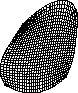
\includegraphics[width=0.9\textwidth,trim=0 0 8mm 1cm, clip]{images/parallel_fiber_estimation/31x31fibers_l2_m0_2In_dirichlet.pdf}
    \caption{Result for parameters $l_\text{max}=2, m=0$, i.e., without interpolation.}%
    \label{fig:31x31_l2_center}%
  \end{subfigure}   
   
  \caption{Comparison of generated meshes of the biceps with different maximum recursion levels $l_\text{max}$. A lower left portion of the full mesh with $31 \times 31$ fibers is shown.}%
  \label{fig:different_recursion_levels}%
\end{figure}%

\begin{figure}%
  \centering%
  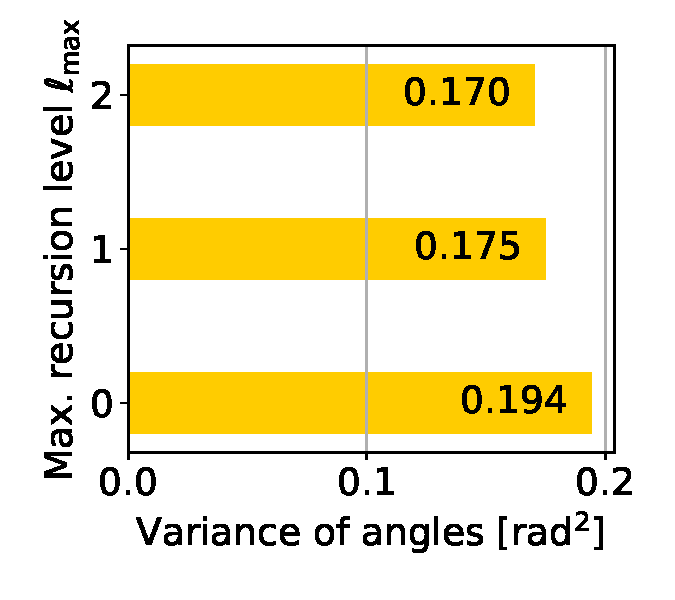
\includegraphics[height=6cm]{images/parallel_fiber_estimation/mesh_quality_recursion_level.pdf}%
  \caption{Variance of the element angles for meshes with the same number of $31 \times 31$ fibers, but created by different recursion levels $\ell_\text{max}$. The parameters correspond to the third row of \cref{tab:file_sizes}. A lower variance means better mesh quality.}%
  \label{fig:2mesh_quality}%
\end{figure}%

\subsection{Effect of Mesh Quality Parameters}\label{sec:mesh_generation_mesh_quality_parameters}

In addition to the parameters that affect the resulting mesh sizes, $n_\text{el,x}$, $l_\text{max}$ and $m$, further options exist to tune the behavior of \cref{alg:parallel_algorithm_1} and in result lead to meshes with different quality. These options are described in the following.

The surface that is the input to \cref{sec:parallel_algorithm} can be represented either as triangulation or in parametric form as NURBS surface. The triangulation can either be the result of the image segmentation step or it can be obtained by triangulating a NURBS surface. Thus, if the approximation of the geometry by a smooth spline surface is desired 
it is possible to choose between both options. 

One difference is the resulting runtime. To sample a point on the surface using the NURBS representation, the nonlinear equation has to be inverted using a Newton scheme for each point. This is slower than using the triangulation where rings on $x$-$y$ planes are extracted initially and then equidistantly sampled, as explained in \cref{sec:slicing_of_the_geometry} and \cref{sec:data_structure_of_boundary_points}.

The Laplace problem $Δp=0$ that is solved in every recursion depends on the discretization and mesh resolution on every subdomain.
In addition to the number $n_\text{el,x}$ of elements in $x$ and $y$ directions, the mesh resolution also follows from the number $n_\text{el,z}$ of elements in $z$ direction.

The number of elements in this intermediate mesh is also influenced by the factor $r\in \N$ of the refinement described in \cref{sec:solution_of_the_laplace_problem}. While $r=1$ corresponds to no refinement, for $r>1$ the number of elements is increased by the factor $r^3$.
Note that the output meshes of the algorithm depend on $n_\text{el,x}$ but not on $n_\text{el,z}$ nor $r$ as they are generated later after the process of streamline tracing.

Furthermore, the finite element discretization of the Laplace problem can either use linear or quadratic ansatz functions, leading to the respective linear or quadratic elements in the mesh.
The type of boundary conditions for the Laplace problem in \cref{eq:fiberest_laplace} can be selected among the Neumann boundary conditions given by \cref{eq:fiberest_neumann} or the Dirichlet boundary conditions given by \cref{eq:fiberest_dirichlet}.

After the Laplace problem is solved, the gradient direction $\nabla p(\bfx)$ at a point $\bfx$ in the domain needed for streamline tracing can be determined by two different methods.
Either the gradient vector field is precomputed using finite differences and the nodal values of the solution field $p$ and then evaluated at $\bfx$.
Or the gradient value is directly interpolated at $\bfx$ in the 3D element using a linear combination of the solution values and derivatives of the ansatz functions of the element.

During parallel streamline tracing, the width $n_\text{ghost\_layer\_width}$ of the ghost layer is important. If it is too small, streamlines leave the domain of the process and have to be repaired, i.e., approximated by neighboring streamlines as described in \cref{sec:repair_of_incomplete_streamlines}. We found that a value of $n_\text{ghost\_layer\_width}=2\,r$ is enough and minimizes the number of invalid streamlines leaving the domain. With some parameter combinations, invalid streamlines still occur occasionally. Those result from badly conditioned elements and gradient values with high numerical errors that cannot be fixed by a larger ghost layer.
By including the factor $r$ in the ghost layer width, the actual sizes of the ghost layer is always the same independent of the chosen refinement.

To investigate the effect of all options, a parameter study is conducted in the following. We fix the values of $n_\text{el,x}=4$, $n_\text{el,z}=50$, $m=1$, $l_\text{max}=1$, and $n_\text{ghost\_layer\_width}=2\,r$ and vary all other parameters. The resulting meshes consist of $33 \times 33$ fibers and $31 \times 31$ fibers if the boundary layer is omitted, as described in \cref{sec:postprocessing_of_the_generated_streamlines}. We compare the mesh quality of the 3D meshes that result from the $31 \times 31$ fibers.
As before, the variance of the element angles is used to rate the quality of each resulting mesh.

To identify a parameter combination in the study, a scenario name is composed of one character each for the various options, as explained in the following.
The linear or quadratic formulation of the Laplace problem is indicated by the characters \say{$\ell$} or \say{q}. Neumann and Dirichlet boundary conditions are indicated by \say{N} and \say{D}. The refinement level $r$ is specified by the respective integer value. Finally, \say{g} or \say{s}  indicates whether the precomputed gradient field (\say{g}) is used in  streamline tracing or the solution values (\say{s}) and derivatives of the ansatz functions.

For example, the scenario considered in \cref{fig:different_recursion_levels,fig:2mesh_quality} can be specified as \say{$\ell$D2s}, as it uses the linear mesh with Dirichlet boundary conditions, a refinement factor $r=2$ and the solution values to compute the gradient.

The following study was performed for the biceps geometry in two variants, firstly using the approximated NURBS surface directly and secondly using a triangulation obtained from the NURBS surface. These two variants are indicated by \say{splines} for the NURBS surface and \say{stl} for the STL file containing the triangulation.

%Additionally, also the variance of relative element lengths in the $x$-$y$ planes was computed, using the calculation explained in \cref{sec:mesh_generation_0_results_and_discussion}. Most scenarios yielded a value of \num{2.2e-2}. Scenarios with significantly different values were discarded, as their results contained incomplete streamlines.
\Cref{fig:3mesh_quality} presents the resulting variances of the element angles.
The scenarios are sorted according to their mesh quality score, i.e., the variance of their element angles. This means the results are ordered by improving mesh quality from bottom to top.

\begin{figure}%
  \centering%
  \begin{subfigure}[t]{0.48\textwidth}%
    \centering%
    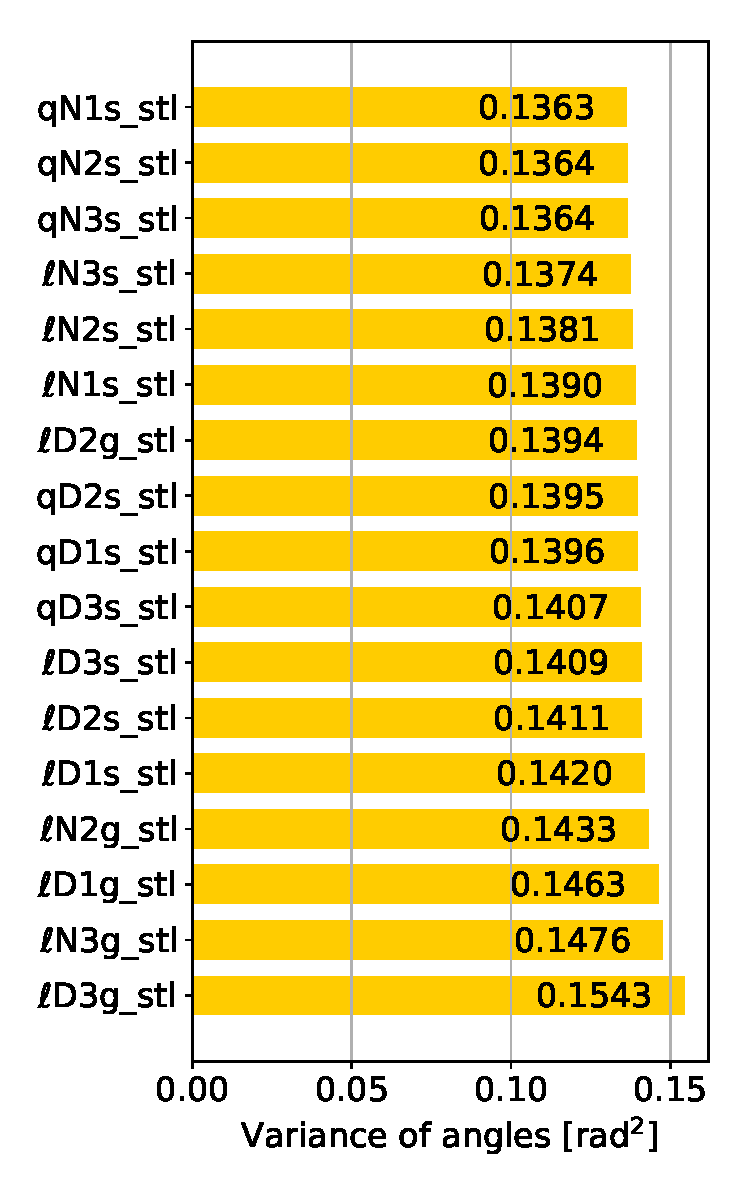
\includegraphics[width=\textwidth]{images/parallel_fiber_estimation/mesh_quality_options_0.pdf}%    
    \caption{Scenario using the surface triangulation.}%
    \label{fig:mesh_quality_options_0}%
  \end{subfigure}
  \begin{subfigure}[t]{0.48\textwidth}%
    \centering%
    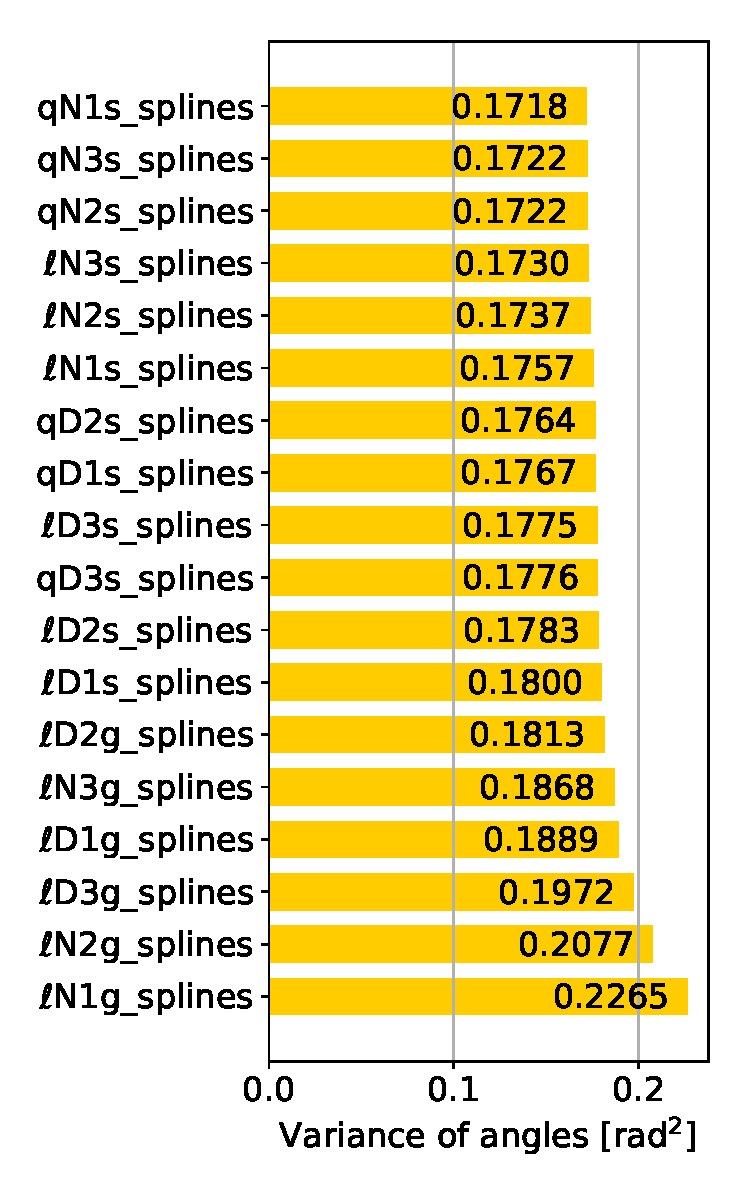
\includegraphics[width=\textwidth]{images/parallel_fiber_estimation/mesh_quality_options_1.pdf}%
    \caption{Scenario using the spline surface.}%
    \label{fig:mesh_quality_options_1}%
  \end{subfigure}
  \caption{Parallel mesh generation algorithm: Comparison of the mesh quality that results from different options in the mesh generation algorithm. A lower variance means better mesh quality.}%
  \label{fig:3mesh_quality}%
\end{figure}%

Two separate plots  for the \say{stl} and \say{splines} scenarios are shown in \cref{fig:mesh_quality_options_0} and \cref{fig:mesh_quality_options_1}.
The two resulting meshes of the best options, \say{qN1s\_stl} and \say{qN1s\_splines} are visualized left and right in \cref{fig:stl_splines_results}.
In the top plane of the muscle belly, it can be seen that the orientation of the mesh is slightly different. This explains the large difference of the angle variance values between the two scenarios in \cref{fig:3mesh_quality}, which are higher for \say{splines} than for \say{stl}. The scores of parameter combinations should therefore only be compared among the same surface representation. A statement regarding which of the two options is better is not reasonable from this data set.

\begin{figure}%
  \centering%
  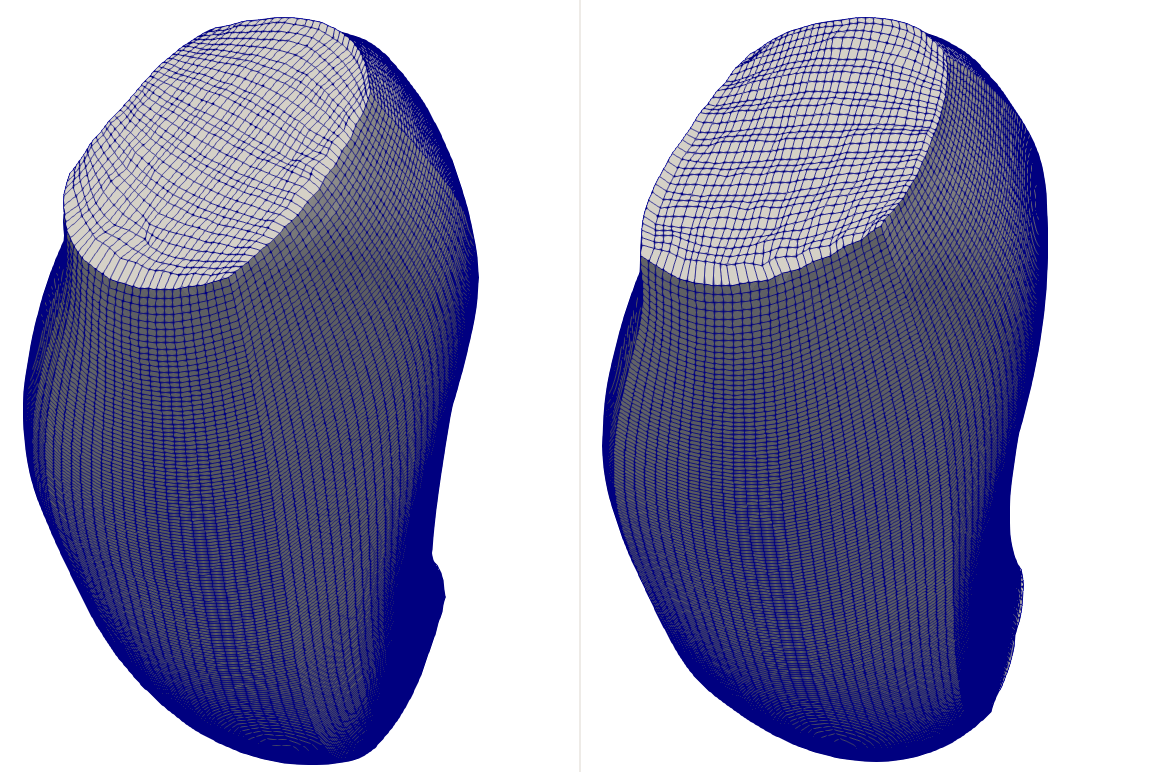
\includegraphics[width=0.8\textwidth]{images/parallel_fiber_estimation/stl_splines_results.png}%
  \caption{Parallel mesh generation algorithm: Results of the scenarios using a surface triangulation (stl, left) and a NURBS surface (splines, right).}%
  \label{fig:stl_splines_results}%
\end{figure}%

The results in \cref{fig:3mesh_quality} show that almost all values are close together, which indicates similar good mesh qualities for different parameter combinations.
Nevertheless, the ranking reveals some differences between the options. 
A comparison of the rankings in the columns for \say{stl} or \say{splines} shows that some parameter choices consistently resulted in better meshes. 
A better result was achieved if Neumann boundary conditions were used (\say{N}) compared to Dirichlet boundary conditions (\say{D}). 
Similarly, quadratic ansatz functions (\say{q}) performed better than linear ansatz functions (\say{$\ell$}). This is reasonable as quadratic ansatz functions yield a higher spatial consistency in the finite element formulation. 

A higher refinement factor $r$ of the internal mesh was beneficial for the cases with linear ansatz functions. For quadratic ansatz functions, the effect of $r$ is less clear. The study shows that no refinement ($r=1$) is often better in this case.
The variant without the precomputed gradient field (\say{s}) performed generally better than the variant with gradient field computation (\say{g}).

However, further studies with different recursion depths showed that the effect of some options also depended on the scenario. For a higher recursion depth, Dirichlet boundary conditions turned out to be more robust in the sense that fewer incomplete streamlines occured.
%Larger refinement factors led to smaller mesh widths and in consequence to a smaller ghost layer for the streamline tracing, which always has a thickness of one element. Thus, more streamlines left their subdomain and became invalid. Therefore, e.g., a smaller value of $r$ yielded better results for $\ell_\text{max}=2$.

In summary, the quadratic formulation (\say{q}) and the streamline tracing using solution values (\say{s}) could be shown to be better options than their alternatives. For a maximum recursion level $\ell_\text{max}=1$, the best parameter combination among the tested combination was \say{qN1s}. In a separate study for $\ell_\text{max}=2$, the combination \say{qD2s} was found to be as robust as \say{qN1s}.
%

\subsection{Postprocessing of the Meshes}

To further improve the mesh quality on every cross section, we apply two more postprocessing steps, one local and one global transformation.
As can be seen in the cross section of \cref{fig:stl_splines_results}, some rows of elements in the generated mesh have zig-zag lines, and not all elements are equally sized. Furthermore, there are almost degenerate elements with small interior angles. 

Thus, we apply a first, local transformation on the mesh. This operation consists of Laplacian smoothing and randomly deflecting points, where interior element angles are smaller than \SI{20}{\degree}. If such deflections result in invalid self-intersecting elements, the self-intersection is resolved, which potentially again introduces small interior angles. The total transformation consists of 25 iterations of alternatingly applying the smoothing step and the improvement step of small interior angles.

An exemplary resulting mesh after this transformation is shown in \cref{fig:mesh47_a}. It can be seen that all lines in the mesh are smooth and almost straight. At the right center of the shown mesh, the effects of the deflection step, which improves small interior angles, can be seen. However, at the left, top and bottom boundary of the mesh, degenerate elements with small interior angles remain. This is especially true for the four mesh points on the boundary that correspond to the corners of the quadrangulation. At these points, elements are present that have two sides that are part of the mesh boundary, forming an interior angle of almost \SI{180}{\degree}. Three points of these elements are located in an almost straight line. As a consequence, the Laplacian smoothing step moves the fourth point of these elements close to this straight line, which adds another large interior angle and degenerates the element. This effect also occors for interior elements of the mesh that are close to these points on the boundary.

\Cref{fig:mesh47_b} shows the detail of the left boundary of the mesh in \cref{fig:mesh47_a}, where this effect can be seen. The area of the elements decreases towards the boundary and the elements get more degenerate in this direction.

As a remedy, we perform the second, global transformation step to counteract this tendency. In this step, most of the points in every cross section of the mesh are translated by a fixed mapping, such that the small elements at the boundary are transformed into elements of better quality.

% plot of function f(r)
\begin{figure}
  \centering%
  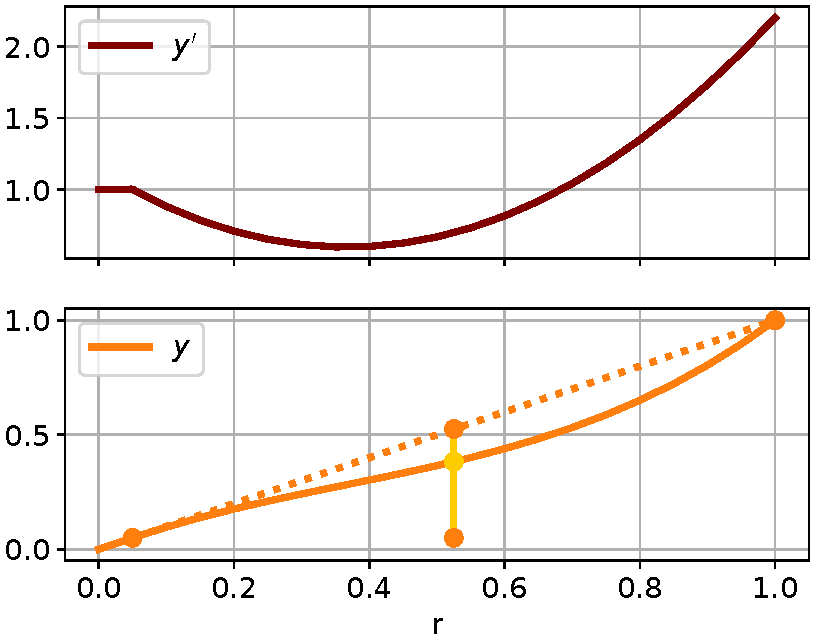
\includegraphics[width=0.5\textwidth]{images/parallel_fiber_estimation/extend_mesh_plot.pdf}%
  \caption{Transformation of a mesh to improve the mesh quality. The depicted function $f$ transforms the elements in radial direction.}%
  \label{fig:extend_mesh_plot}%
\end{figure}%

Each mesh point on a cross section of the mesh is represented by polar coordinates $(r,\varphi)$. The radius $r$ is transformed according to the function $r_\text{new} = y(r_\text{old})$ that is depicted in the lower plot of \cref{fig:extend_mesh_plot}. This piecewise defined function $f\in \CC^1([0,1]\to [0,1])$ is linear for $x\in [0,s]$ and a polynomial of degree 3 for $x \in [s,1]$. It passes through the yellow point in \cref{fig:extend_mesh_plot}, which in $x$ direction is at the center of the interval $[s,1]$ and in $y$ direction is at fraction $\alpha$ of the shown yellow line.
The parameter $\alpha$ controls the extent, to which the mesh is transformed in radial direction. The parameter $s$ specifies the size of a region around the center of the mesh where no transformation occurs. We obtain good results by choosing $s=0.05$ and $\alpha=0.7$. The resulting function takes the form $f(r) = 1.330\,r^3 - 1.463\,r^2 + 1.136\,r - 0.003$.

The first derivative $f'(x)$ of this function is shown in the upper plot of \cref{fig:extend_mesh_plot}. It quantifies the amount of extension or compression of the mesh elements in radial direction. The right side of the plot corresponds to the outer boundary of the mesh. There, the elements are extended, since $f'(r) > 0$. To compensate this extension, the elements have to be compressed towards the interior of the mesh  where $f'(r) < 0$. The range of $r \in [0,s]$ corresponds to the region in the interior of the mesh that is not transformed.

The points of the mesh are transformed in radial direction by adjusting their coordinate $r$ and not transformed in circumferential direction, i.e., the angle $\varphi$ remains constant. However, the application of the function $f$ on $r$ is additionally modulated by a piecewise sine function depending on $\varphi$. The transformation $f$ is only fully applied at the four radii corresponding to the described special points on the boundary, around which the degenerated elements occur. In between these lines, the transformation is reduced and some points of the mesh are not transformed at all.

\Cref{fig:mesh47_b} shows the mesh of \cref{fig:mesh47_a} after this transformation has been applied. \Cref{fig:mesh47b_} shows the extract of the mesh from the left boundary that corresponds to the same extract of the original mesh in \cref{fig:mesh47a_}.
It can be seen that the quality of the elements is improved close to the boundary. The area of the rectangles is now approximately equal and no small interior angles occur.

In \cref{fig:mesh_47ab}, the previous and the transformed mesh are overlayed to show the regions that remain unmodified. The unmodified parts form a \say{cross} shape that touches the boundary at the regions where the mesh quality is also good in the original mesh.

% original and transformed mesh
\begin{figure}
  \centering%
  \begin{tabular}{cc}
    \begin{subfigure}[t]{0.30\textwidth}%
      \centering%
      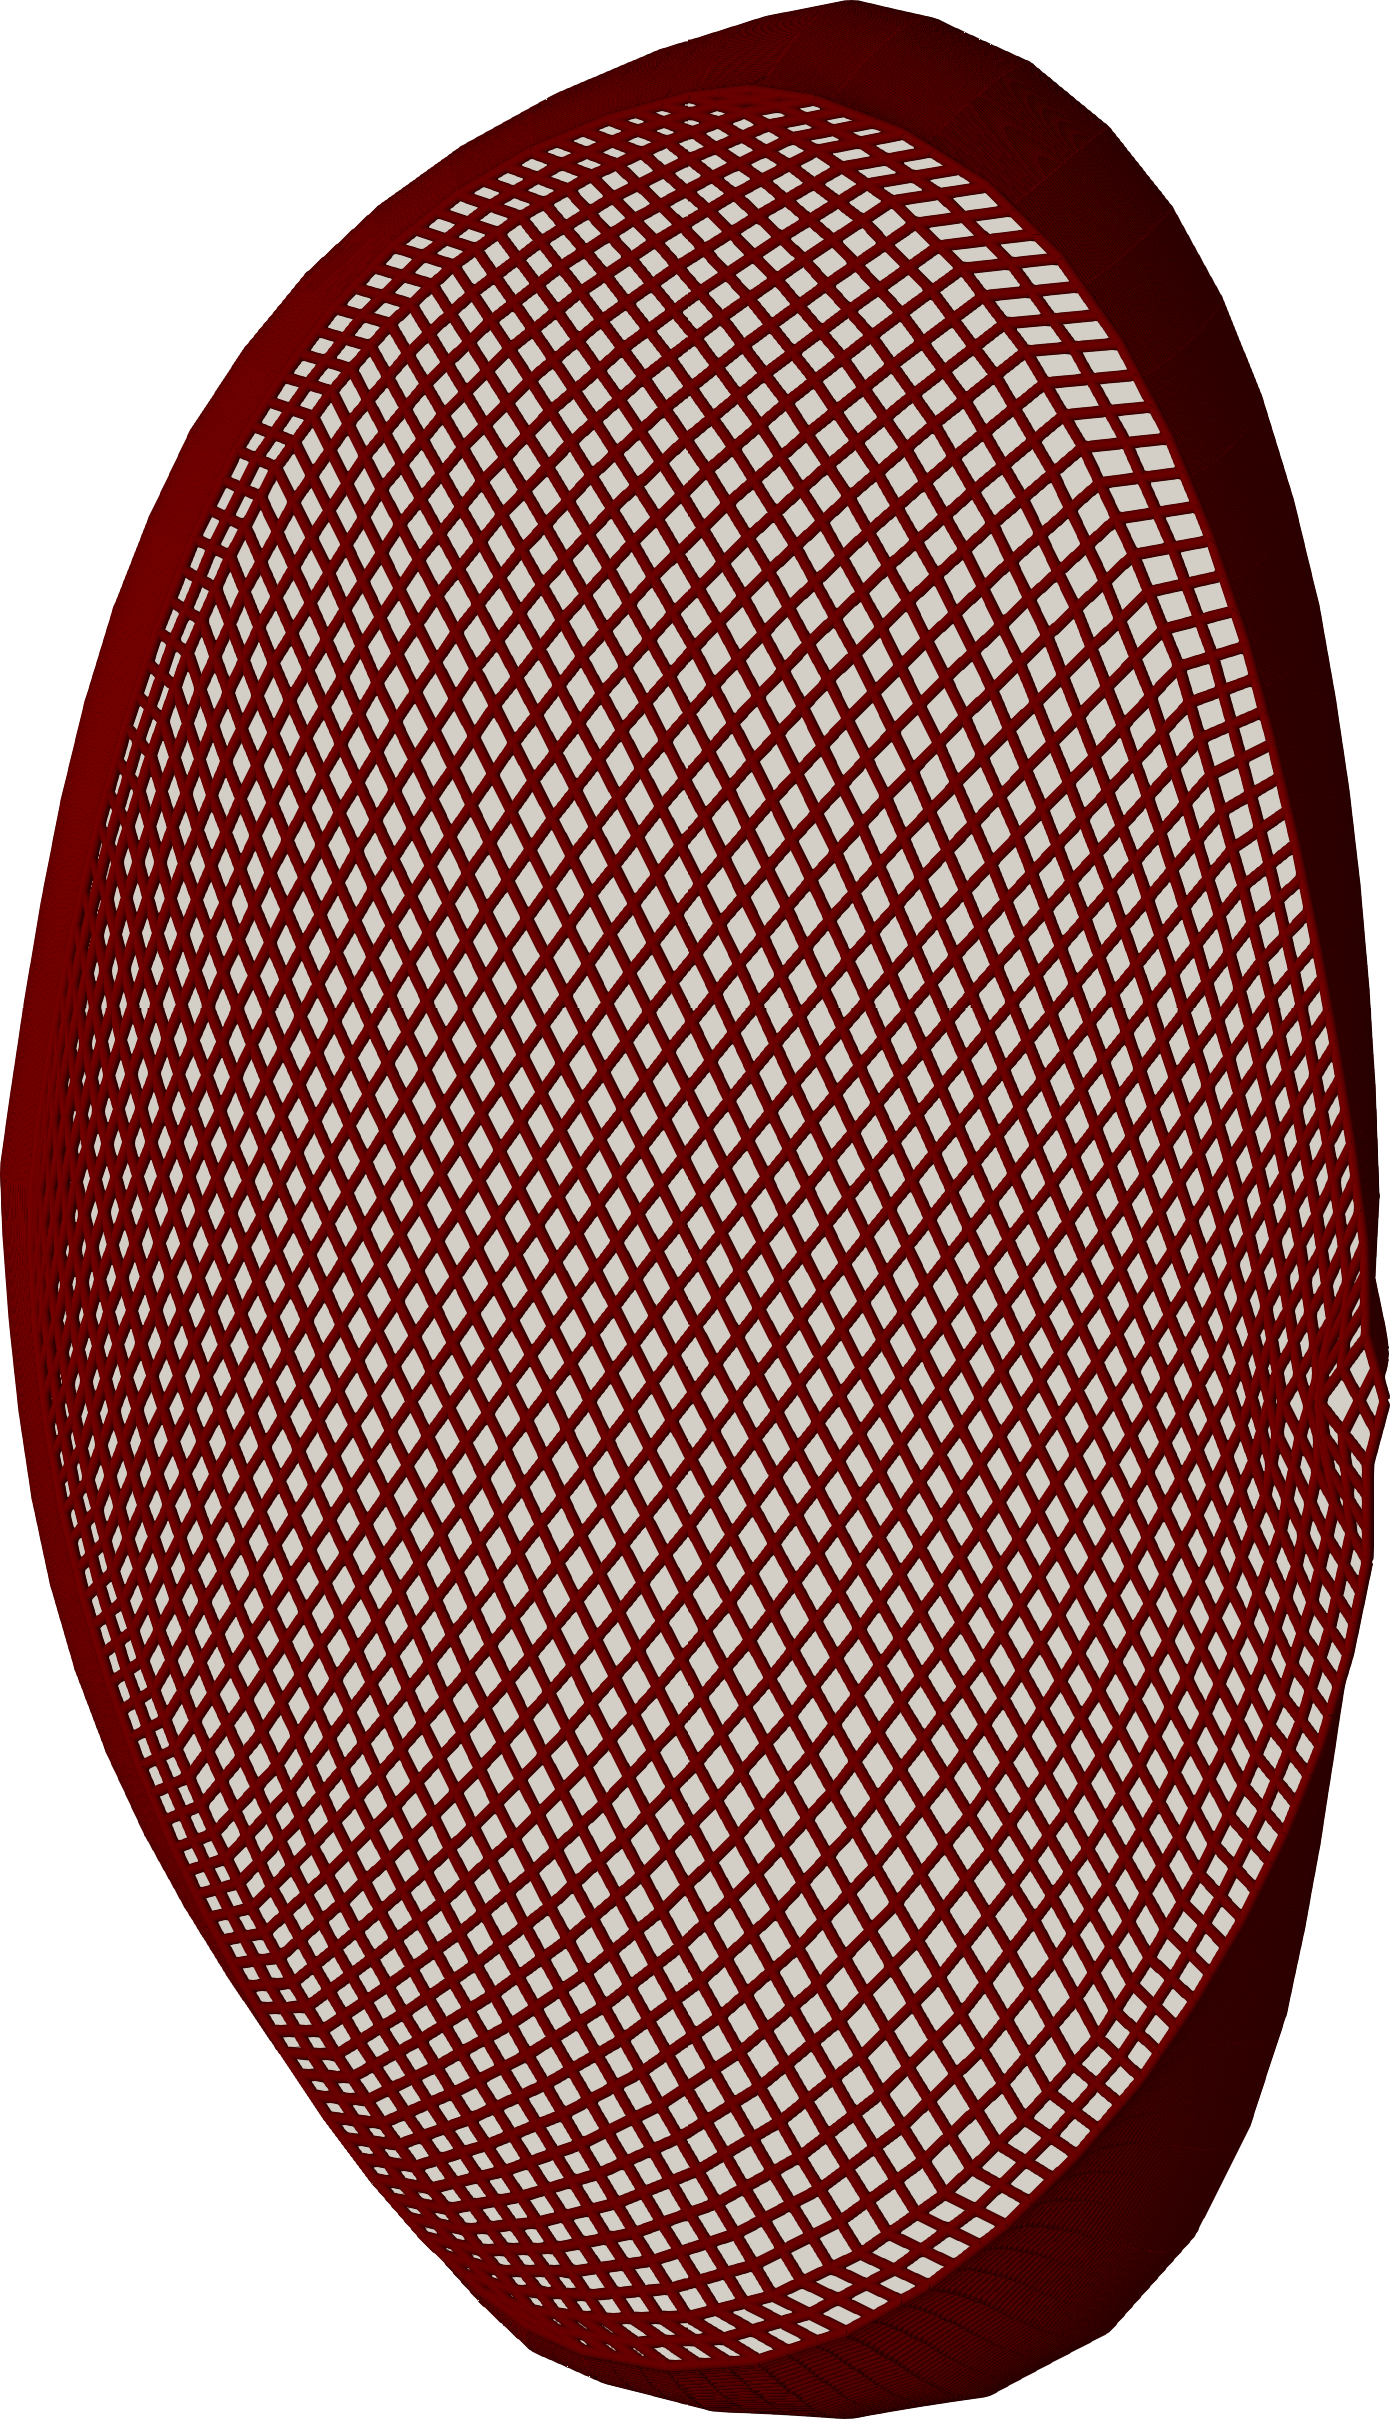
\includegraphics[width=\textwidth]{images/parallel_fiber_estimation/mesh47_a.png}%
      \caption{Original mesh at the upper-most cross section of the muscle.}%
      \label{fig:mesh47_a}%
    \end{subfigure}
    &
    \begin{subfigure}[t]{0.30\textwidth}%
      \centering%
      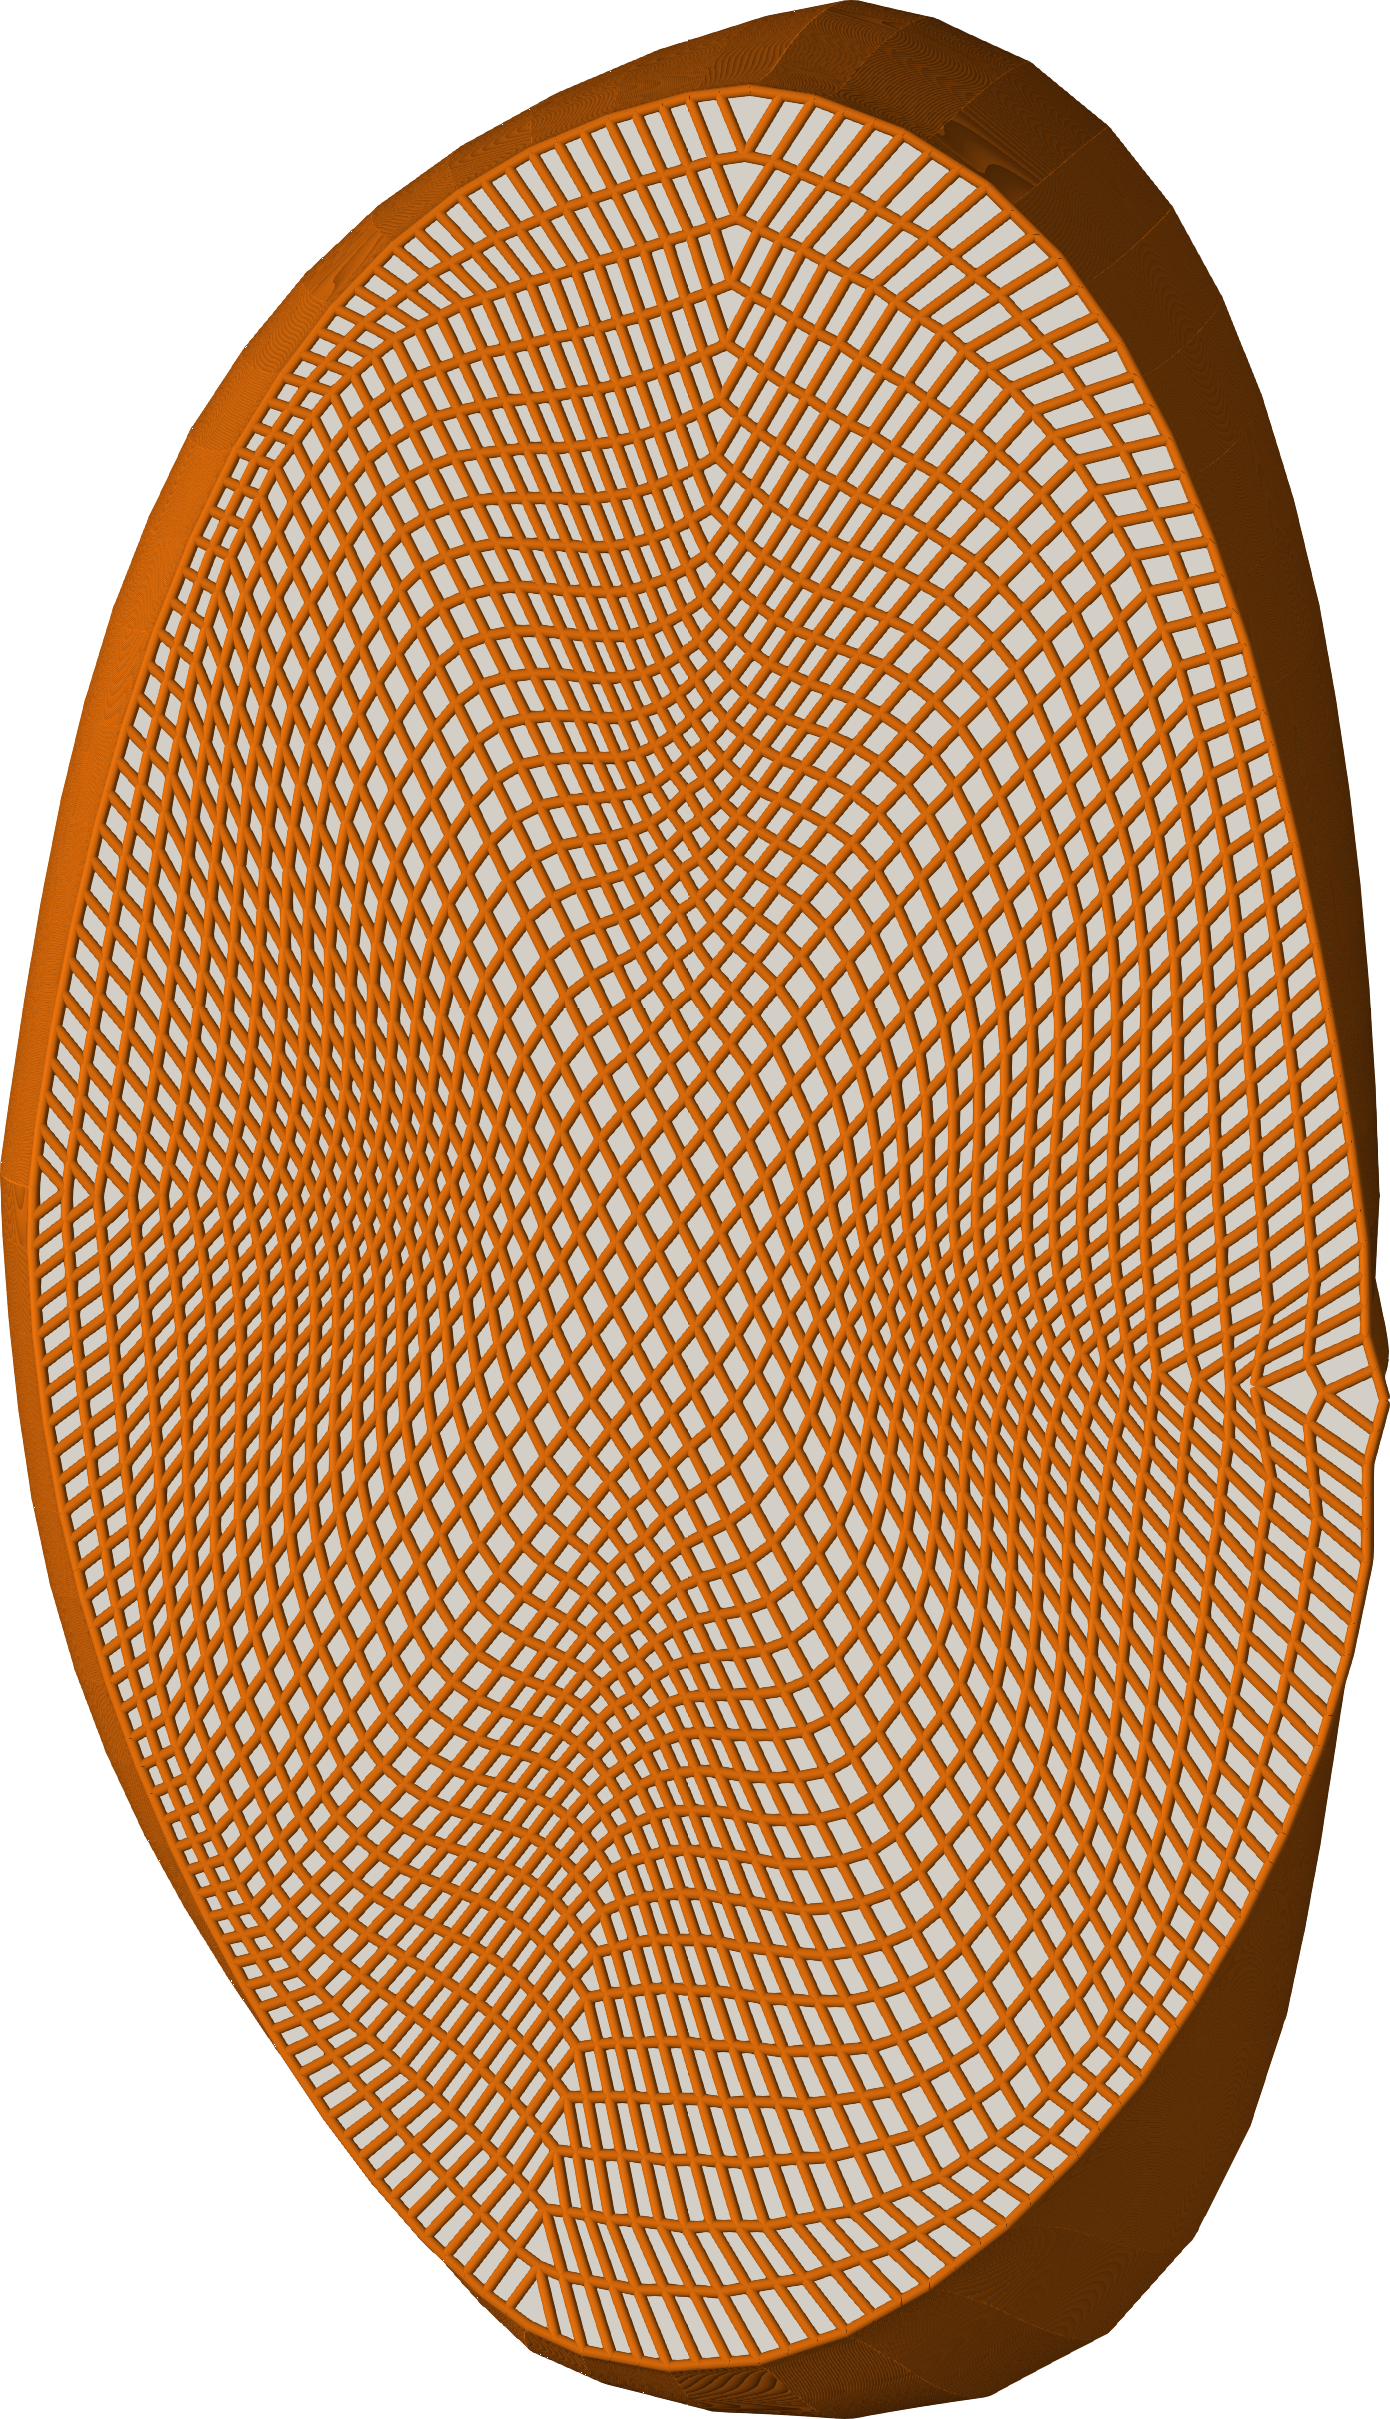
\includegraphics[width=\textwidth]{images/parallel_fiber_estimation/mesh47_b.png}
      \caption{Transformed mesh with better mesh quality.}%
      \label{fig:mesh47_b}%
    \end{subfigure}  
    \\
    \begin{subfigure}[t]{0.48\textwidth}%
      \centering%
      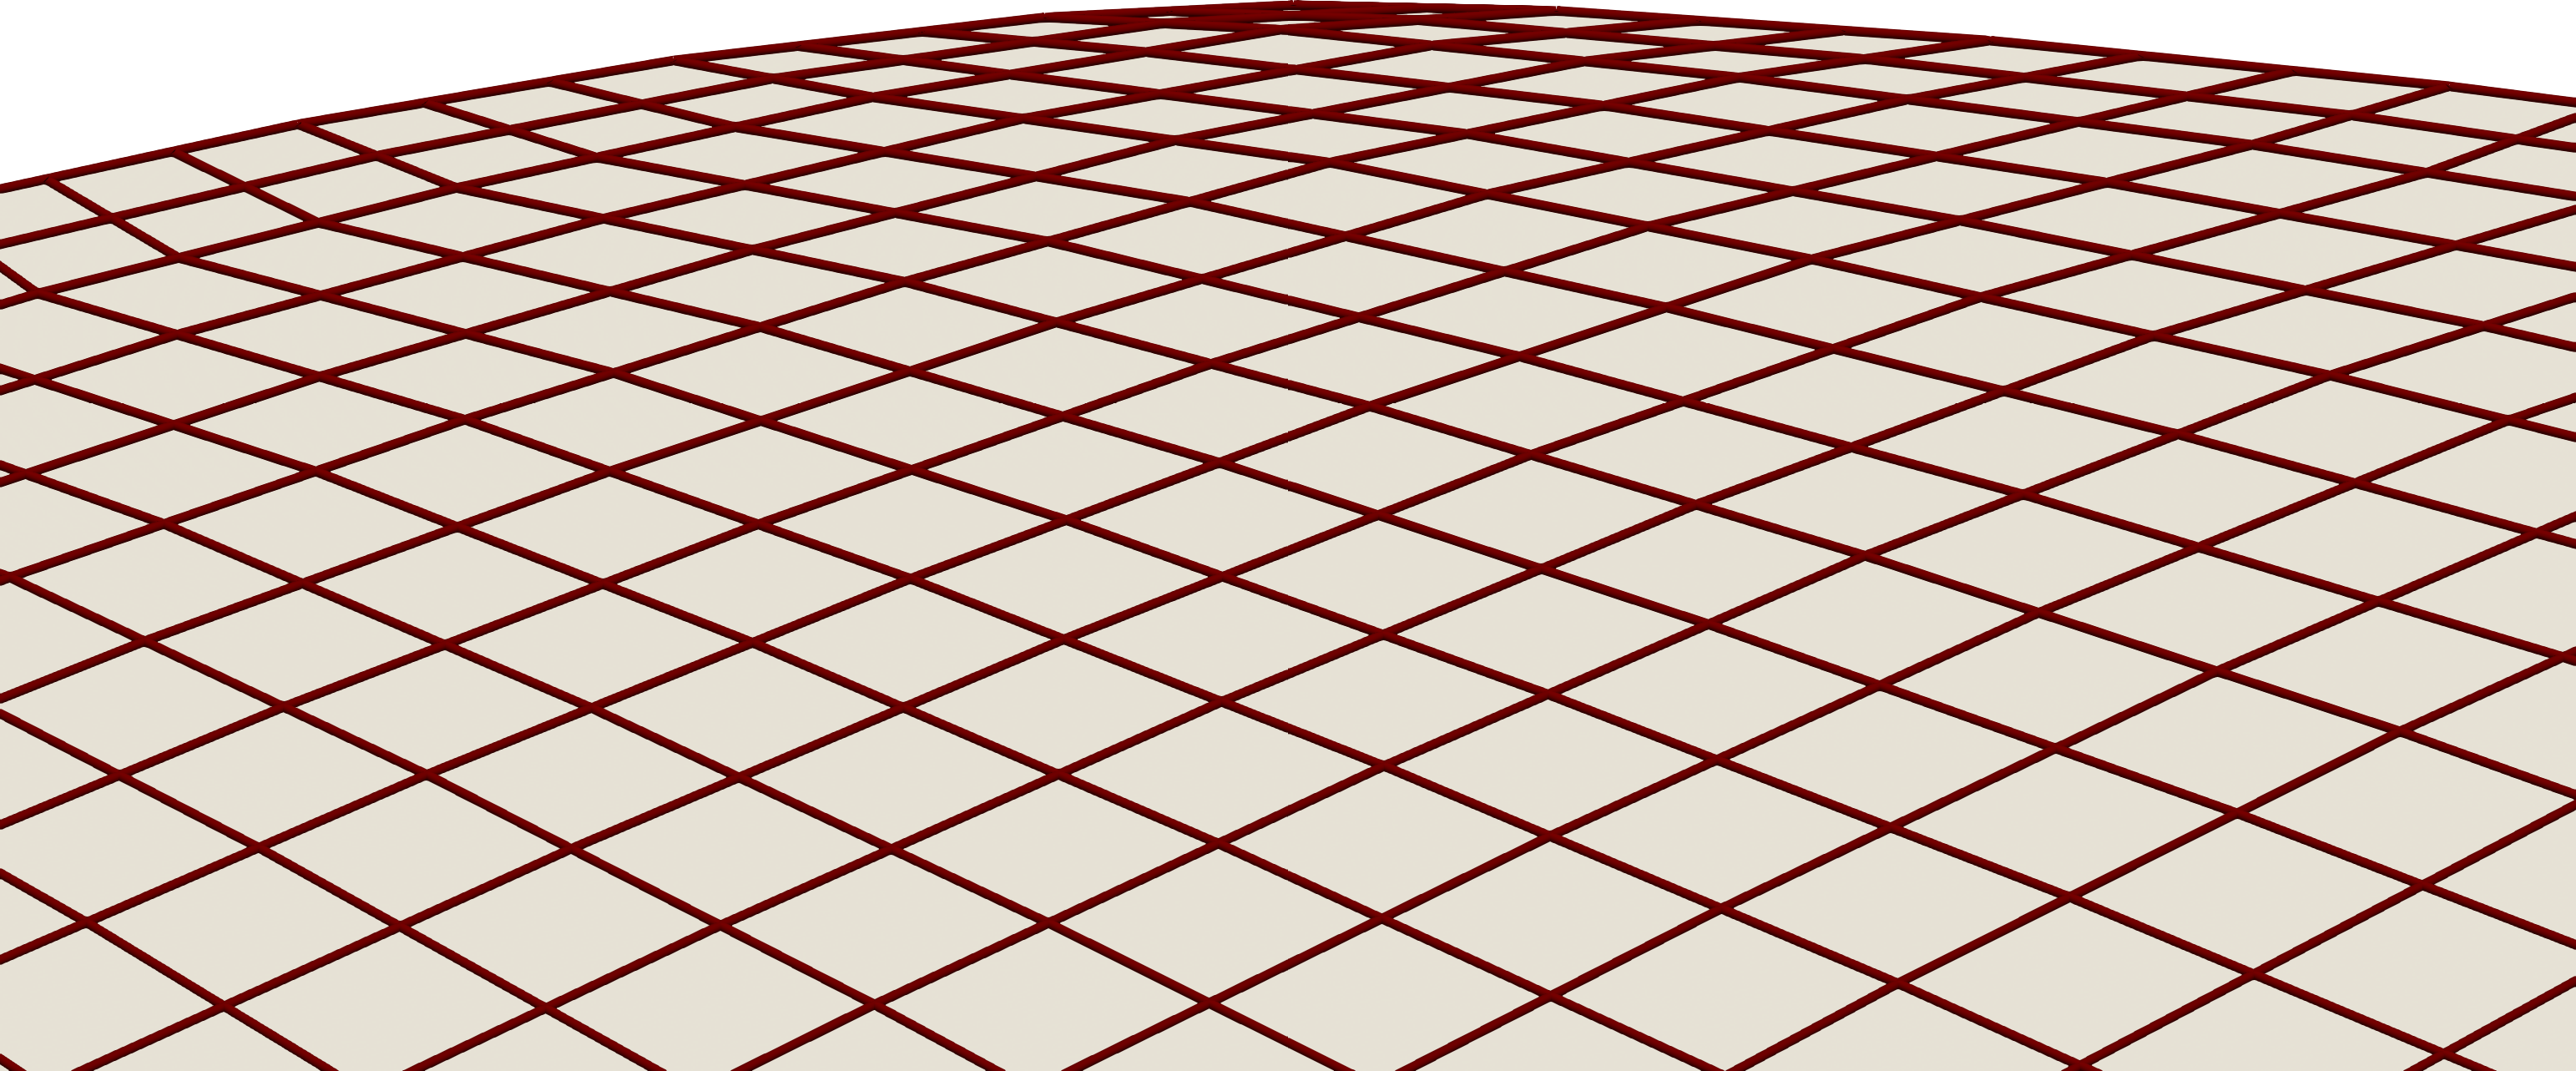
\includegraphics[width=\textwidth]{images/parallel_fiber_estimation/mesh47a_.png}
      \caption{Extract at the left boundary of the original mesh in (a), rotated clockwise by \SI{90}{\degree}.}%
      \label{fig:mesh47a_}%
    \end{subfigure}
    &
    \begin{subfigure}[t]{0.48\textwidth}%
      \centering%
      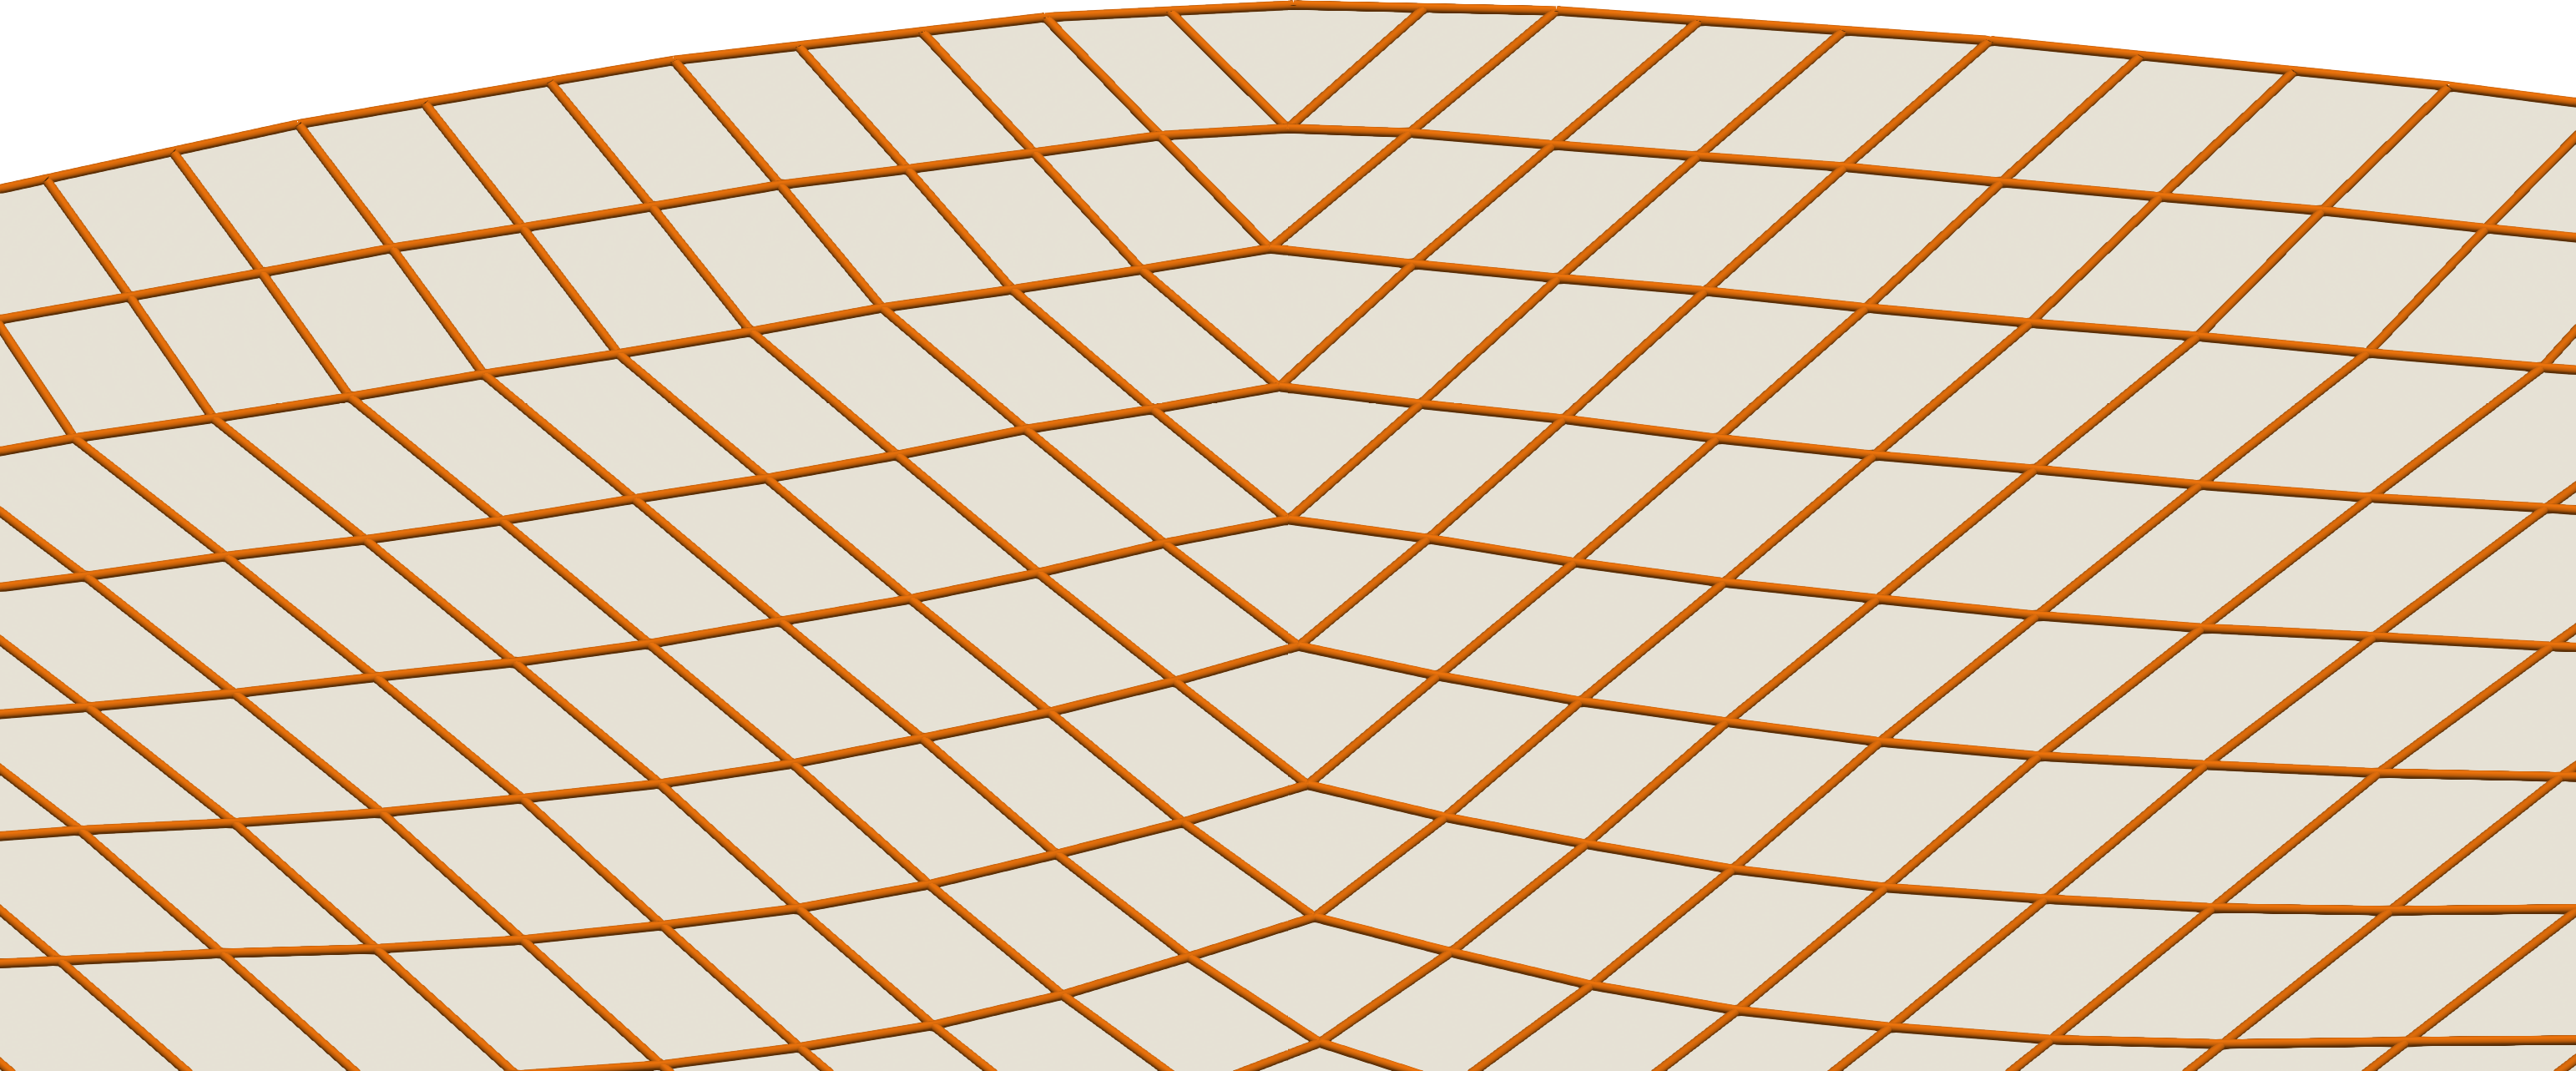
\includegraphics[width=\textwidth]{images/parallel_fiber_estimation/mesh47b_.png}
      \caption{Analog extract to (c) of the transformed mesh (b).}%
      \label{fig:mesh47b_}%
    \end{subfigure}    
  \end{tabular}
  \begin{subfigure}[t]{0.7\textwidth}%
    \centering%
    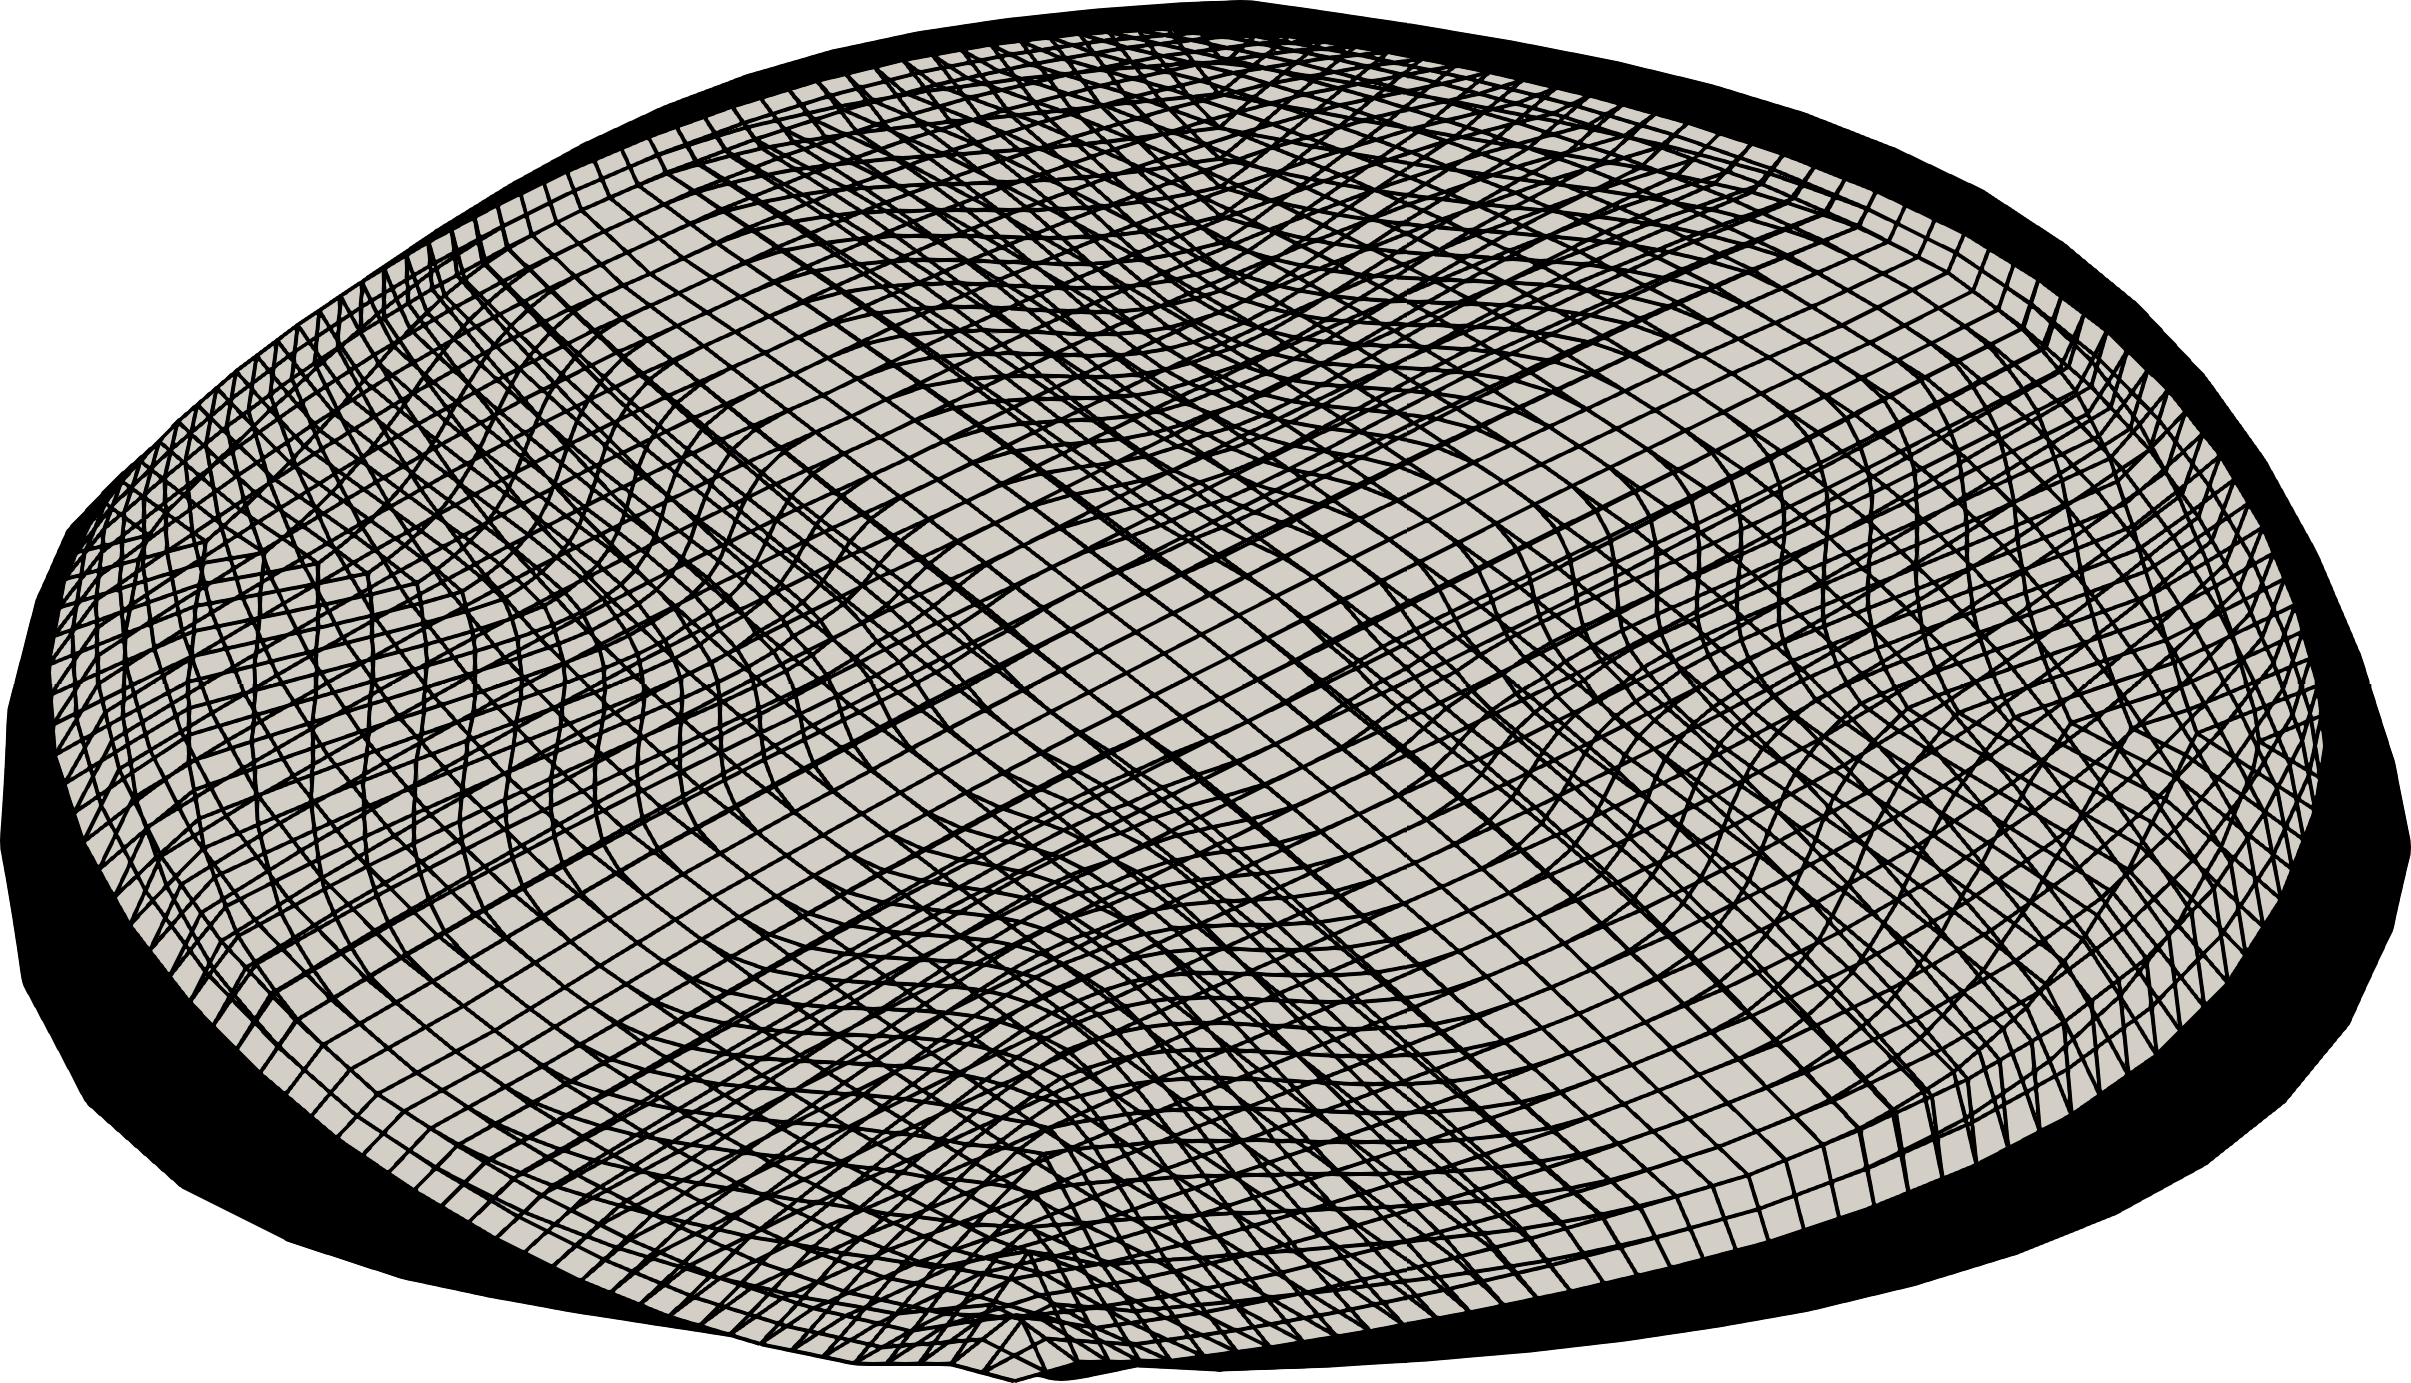
\includegraphics[width=\textwidth]{images/parallel_fiber_estimation/mesh_47ab.png}
    \caption{Overlay of the original mesh (a) and the transformed mesh (b), rotated clockwise by \SI{90}{\degree}. The unmodified regions can be seen.}%
    \label{fig:mesh_47ab}%
  \end{subfigure}
  \caption{Transformation of a biceps mesh with $47\times 47$ points to improve the mesh quality.}%
  \label{fig:mesh47}%
\end{figure}%

%
\subsection{Usage of the Generated Meshes in Simulations}

In some biomechanical simulations, also a body fat and skin layer ontop of the muscle is considered. In this case, an appropriate mesh is required that is attached to the muscle mesh and seamlessly matches the elements of the muscle mesh. The construction of such a mesh is discussed later in \cref{sec:construction_and_partitioning_of_the_mesh} together with the parallel partitioning.

A visualization of such a parallel setting is given in \cref{fig:partitioning_biceps}. Tendons connect the muscle belly of the biceps brachii muscle to the humerus and ulna bones at the top left and bottom, respectively. The muscle mesh consists of fibers that are colored according to a parallel partitioning. In a parallel partitioning, every process contributes calculations only on its associated spatial subdomain to the overall computation. At the right side of the muscle, a layer of adipose tissue is attached to the muscle belly. This layer is needed, if electromyography on the skin surface is simulated. 

% fat layer mesh and partitioning
\begin{figure}
  \centering%
  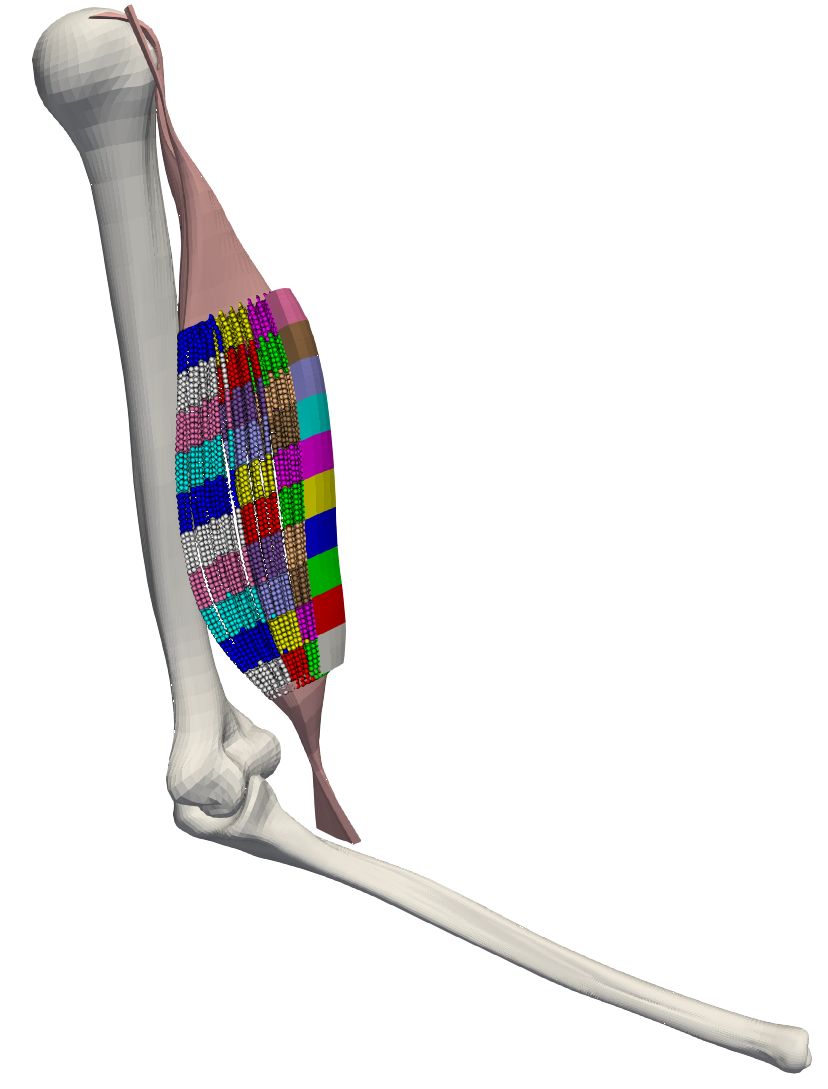
\includegraphics[width=\textwidth]{images/parallel_fiber_estimation/partitioning_biceps.png}%
  \caption{Summary visualization of the simulation setup in this work (I): Biceps muscle with tendons and bones, parallel partitioned fibers and a fat layer mesh.}%
  \label{fig:partitioning_biceps}%
\end{figure}%

\Cref{fig:muscle_meshes_raytrace} shows another use case of various meshes in a multi-scale simulation model. The muscle is cut open for visualization purposes. The figure depicts numerous muscle fibers in the upper part of the muscle belly. The fibers are colored according to simulation results of the electric mebrane potential, which  is responsible for the activation of the muscle. The lower part of the muscle shows elements of the 3D mesh. The coloring corresponds to the electric potential, that is measured during intramuscular electromyography in the interior of the muscle or during surface electrophysiology on the outside of the muscle.

% 3D and 1D meshes
\begin{figure}
  \centering%
  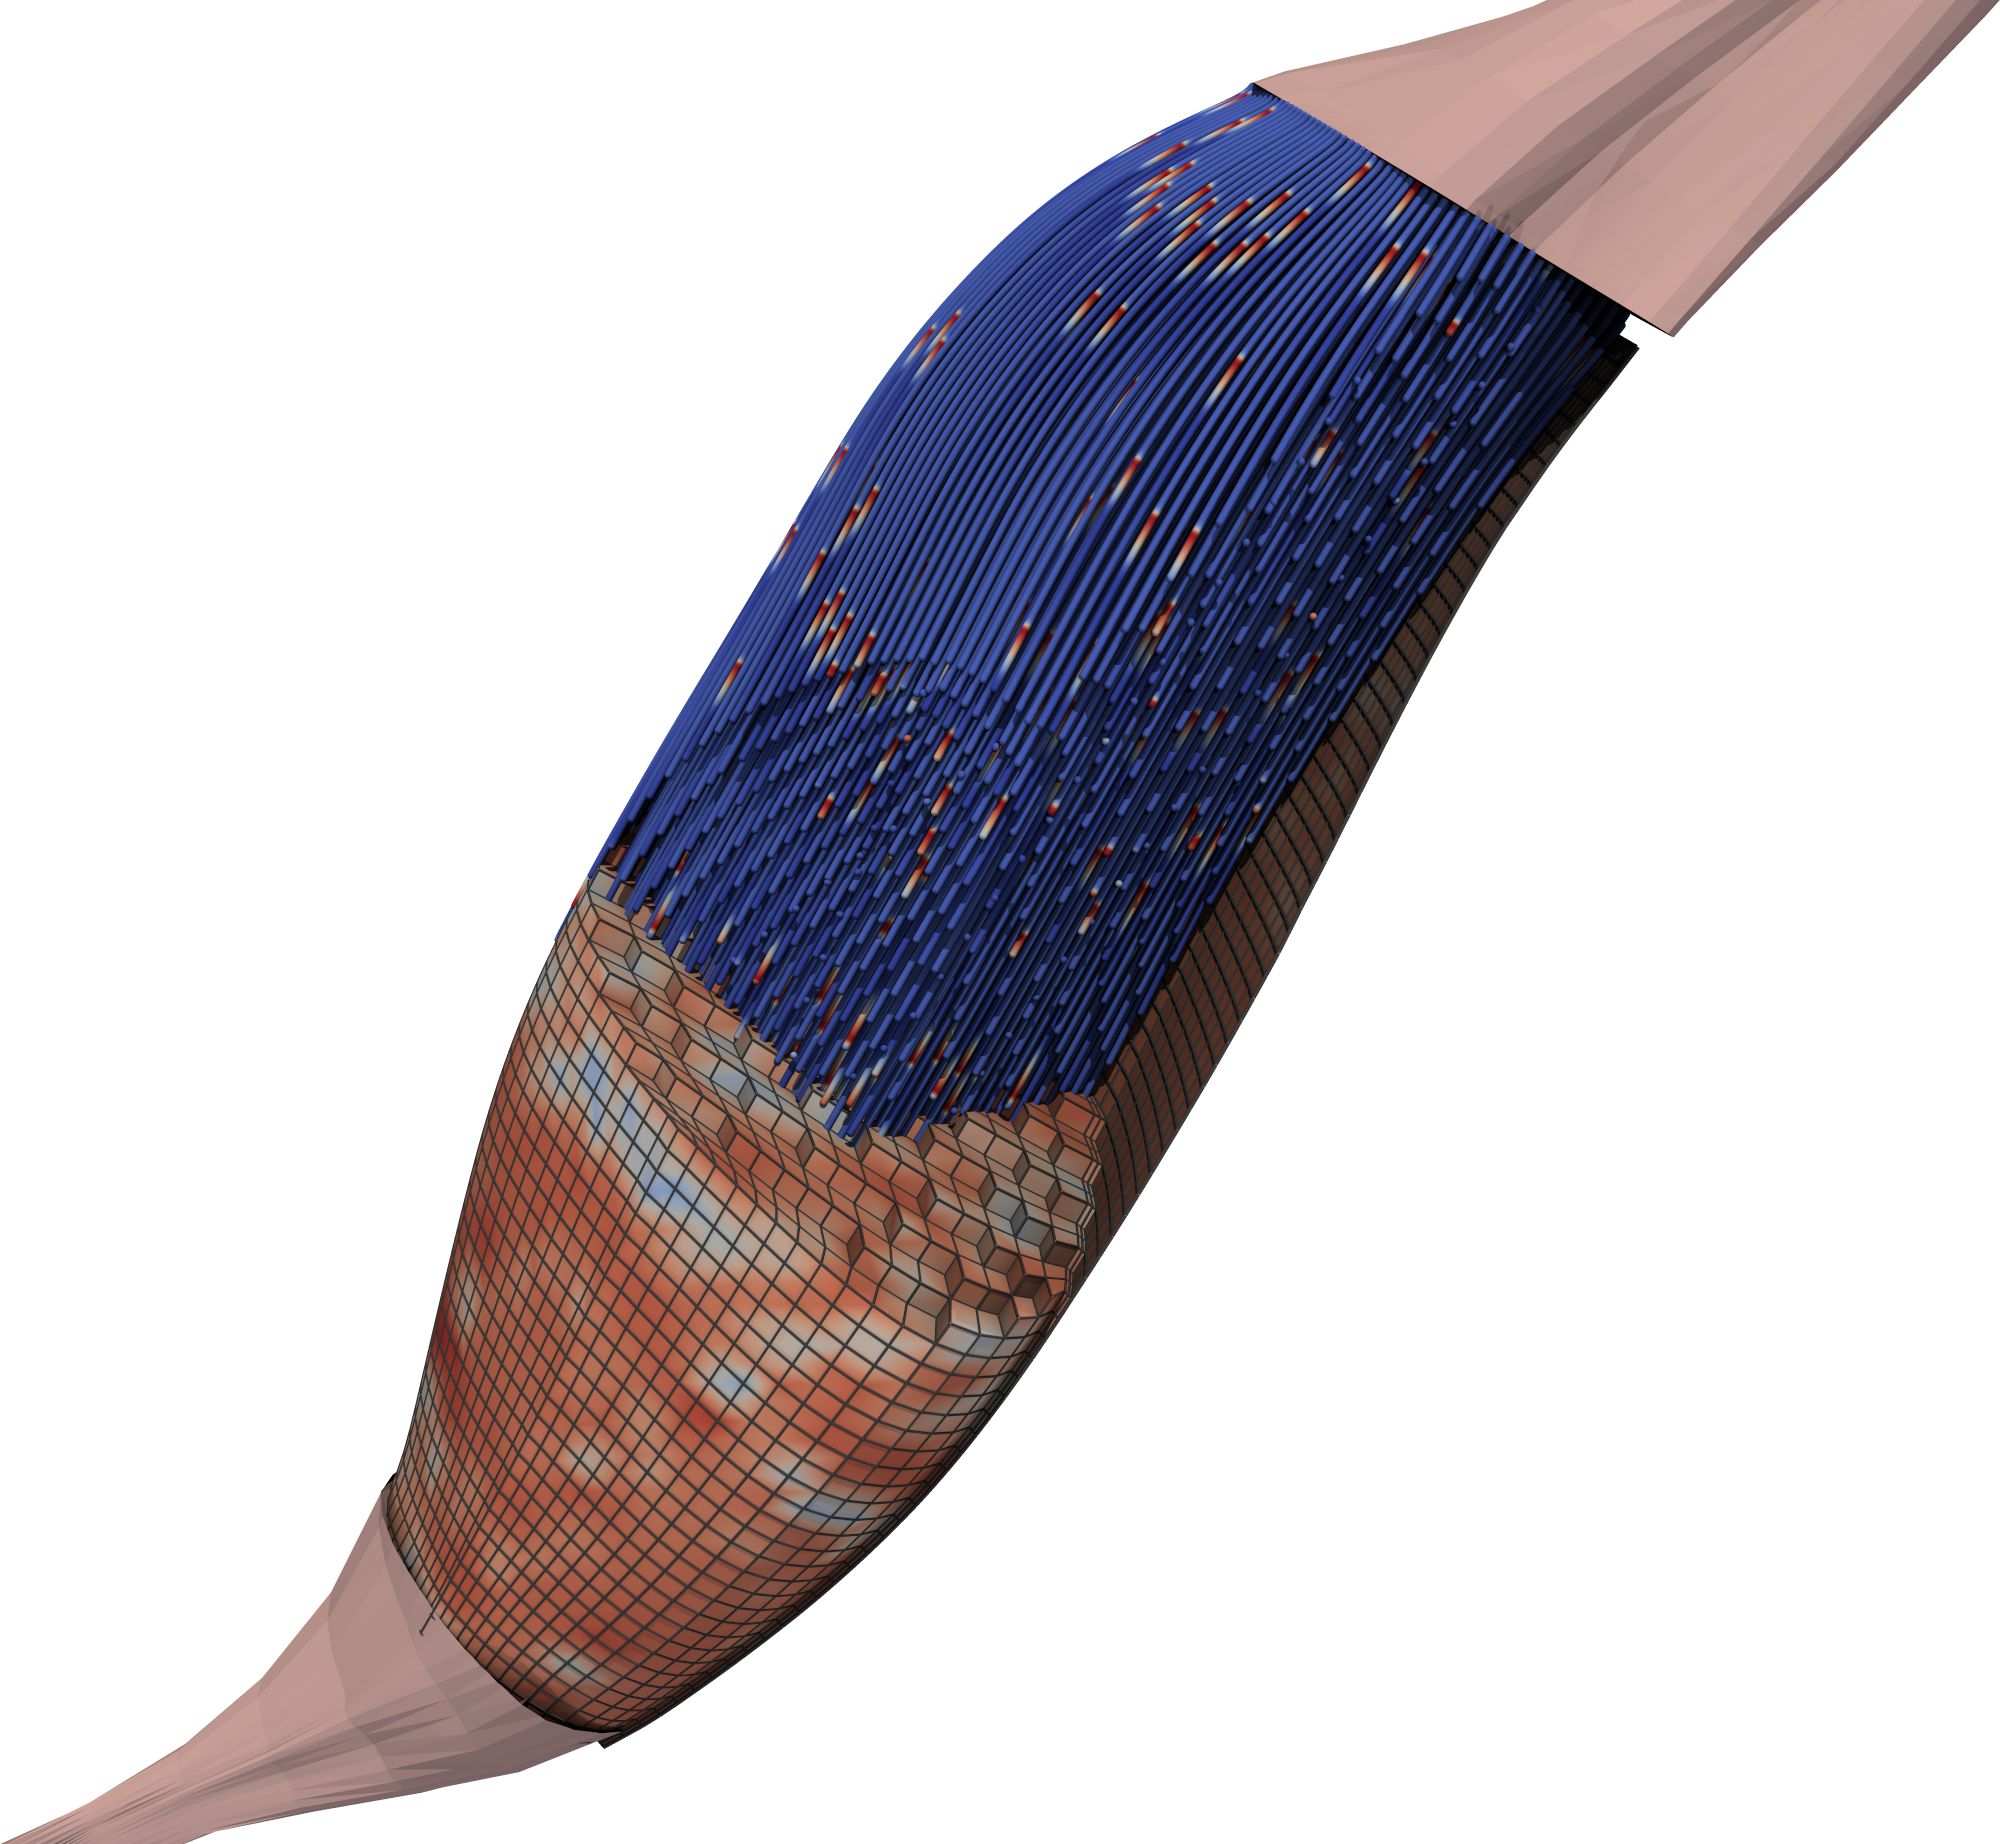
\includegraphics[width=\textwidth]{images/parallel_fiber_estimation/muscle_meshes_raytrace.png}%
  \caption{Summary visualization of the simulation setup in this work (II): Muscle fibers in the upper part and 3D mesh elements in the lower part of the muscle belly.}%
  \label{fig:muscle_meshes_raytrace}%
\end{figure}
\clearpage


%19G     resulting_meshes
%The created meshes have been written to "resulting_meshes". Now you can copy these files to the examples/electrophysiology/input directory

%real    1047m29.662s
%user    3970m33.404s
%sys     4m6.717s


\label{sec:repro_tendon_meshes}
\begin{reproduce}
  The parallel algorithm is implemented in the example \code{parallel_fiber_estimation}. 
  Numerous parameters can be set on the command line. After compilation, run the program as follows to get a description of all available options.
  \begin{lstlisting}[columns=fullflexible,breaklines=true,postbreak=\mbox{\textcolor{gray}{$\hookrightarrow$}\space}]
    cd $\$$OPENDIHU_HOME/examples/fiber_tracing/parallel_fiber_estimation/build_release
    ./generate ../settings_generate.py --help
  \end{lstlisting}
  Running the program without options and \code{--help} uses sensible default values. A given surface triangulation of the biceps muscle gets used by default. To compute the examples shown in this section, use and adjust the following script that runs the \code{generate} program and computes the mesh quality:
  \begin{lstlisting}[columns=fullflexible,breaklines=true,postbreak=\mbox{\textcolor{gray}{$\hookrightarrow$}\space}]
    cd $\$$OPENDIHU_HOME/examples/fiber_tracing/parallel_fiber_estimation/build_release
    ../run.sh
  \end{lstlisting}
  Computation of mesh and file sizes as shown in \cref{tab:file_sizes} can be done using the \emph{compute\_sizes.py} script.
  
  While the previously given commands are good for exploring the algorithms, generation of the meshes used for the simulation involves some more steps. Dedicated scripts exist that perform all steps and call the algorithms with the proper parameters.
  Starting from the STL file extracted from cmgui, as explained in \cref{sec:surf_extr}, the next steps are: 
  \begin{itemize}[leftmargin=1cm]
  \item[(i)] Scale the points from millimeters (used in the Visible Human dataset) to centimeters (used in the simulation), 
  \item[(ii)] remove the interior triangles, 
  \item[(iii)] translate the mesh such that the bounding box begins at $z=0$, this is needed for the programs used in the next steps, 
  \item[(iv)] create the spline surface representation as explained in \cref{sec:nurbs}, 
  \item[(v)] compile and run the \opendihu{} programs to create the binary files of the 3D mesh and the 1D fibers meshes, the algorithm in \cref{sec:parallel_algorithm} is used, 
  \item[(vi)] adjust the indexing and undo the translation in (iii), \item[(vii)] refine the created meshes of key fibers by different numbers $m$ of fine grid fibers, in total 10 different mesh sizes are created for differently refined simulations, 
  \item[(viii)] create meshes for the fat layer $\Omega_B$ ontop of the muscle surface, also in 10 different resolutions.
  \end{itemize}
  
  Two scripts are given for the biceps brachii and triceps brachii muscles. They perform all listed steps and also create intermediate output files that can be used to understand the process. Some steps are automatically skipped if the resulting output file already exists from a previous run. This is especially helpful for the removal of the interior triangles from the initial file which takes nearly a full day.
  
  A third scripts creates three meshes $\Omega_{T,i}$ for the tendons of the biceps muscle, as visualized in \cref{fig:tendon_meshes}. At the bottom, a single tendon mesh is created whereas at the top, two seperate tendons exist. The script involves numerous rotation and cropping operations of the initial surface, before the algorithm of \cref{sec:ser_alg_meshes} is executed. The three output files of the tendon meshes have the same file format as the muscle meshes. The files have the extension \emph{.bin} for \say{binary}. The script \code{examine_bin_fibers.py} can be used to debug the created binary files.
  
  The three scripts can be executed as follows:
  \begin{lstlisting}[columns=fullflexible,breaklines=true,postbreak=\mbox{\textcolor{gray}{$\hookrightarrow$}\space}]
    cd $\$$OPENDIHU_HOME/examples/electrophysiology/meshes
    ./process_meshes_biceps.sh
    ./process_meshes_triceps.sh
    ./process_meshes_tendons.sh
  \end{lstlisting}
  The output can be found in the subdirectory \code{processed_meshes}. For the total output about \SI{68}{\gibi\byte} of drive space is required, however, the resulting meshes have a size of only \SI{19}{\gibi\byte}. A total runtime of more than a day is to be expected.
  
\end{reproduce}

\section{Conclusion and Future Work}\label{sec:meshes_summary_and_conclusion}

This chapter presented algorithms for creating muscle meshes that are needed for multi-scale simulations of the musculoskeletal system.
For the biceps muscle, 3D meshes for tendons on both ends and the muscle were created. Additionally, 1D fibers meshes were generated that are embedded in the mesh of the muscle. The 3D mesh and the 1D meshes resulting from the parallel algorithm are aligned with each other. This facilitates data mapping between the meshes and reduces numerical errors. All generated meshes are structured, which allows an efficient parallelization.

First, an overview of available meshing software and known algorithms in the literature was given. Very little software tools were capable of generating structured meshes and none fitted our special needs. Therefore, own algorithms were developed to generate meshes starting from medical imaging data.

A workflow was presented to generate a smooth surface triangulation from imaging data. Our base data was the male dataset from the Visible Human Project. Two alternatives within this workflow were presented, where the first alternative executed automatic image segmentation based on morphological operations and the second alternative used semi-automatic segmentation tools from the Physiome project. Then, smooth NURBS surfaces were fitted to the extracted boundaries of the muscle volumes.

Next, a novel algorithm to create structured meshes from a triangulated muscle surface was presented. The algorithm used harmonic maps on 2D slices in combination with regular grids in a parameter space to achieve good mesh quality. A method of computing streamlines in a divergence-free vector field to estimate muscle fibers, which is established in the literature, was used. It allowed to embed 1D meshes for muscle fibers in the created 3D meshes of the muscle. Numerical experiments tested and evaluated different choices of triangulation and quadrangulation schemes for the 2D cross section and reference domains in our algorithm.

Next, a parallelized algorithm was introduced that was based on our first, serial algorithm. The algorithm used distributed memory parallelism and provided the same features as the serial algorithm, having the same formats for input and output. The difference was that it constructed a fine, partitioned mesh for streamline tracing that was distributed over all employed processes. Thus, it was possible to create finer meshes using more compute nodes. Differently resolved meshes of the biceps and triceps muscle volumes and muscle fibers were created using this algorithm. The superiority of the parallel algorithm using a higher number of processes compared to the serial execution was explained and demonstrated in a numerical experiment. Several options to fine-tune the algorithm were evaluated. Postprocessing methods were described that improved the mesh quality of the resulting meshes.

The presented algorithms and their implementation in \opendihu{} are the basis for further computations within this work. They are used to generate structured hexahedral meshes with good mesh quality. These meshes are required for efficient, parallel finite element simulations of various aspects of the neuromuscular system.

The presented algorithms are specialized for fusiform muscles and require the muscle geometry to be oriented along one coordinate axis (the $z$ axis) in order to generate a structured mesh  that comprises planar slices that are normal to that direction.
The algorithms can also be applied to any tubular surface geometry of more complex muscles and will construct the corresponding structured 3D mesh. The generated 1D fiber meshes, however, are only valid for muscles, where the approach of streamline tracing through the solution of the Laplacian potential flow problem with boundary conditions at the bottom and top ends of the muscle can be applied.
In literature, this approach has been successfully used for various muscles with more complex fiber architectures, such as the tibialis anterior, gluteus maximus and deltoid muscles \cite{Choi2013}. However, the locations where boundary conditions were prescribed was not always at the bottom and top ends of the muscle.

If in future work muscles with more complex layouts should be simulated, the approach could be as follows. Depending on the complexity of the outer geometry, first the presented algorithms (either \cref{alg:serial_algorithm_1,alg:serial_algorithm_2} or \cref{alg:parallel_algorithm_1}) can be used to create a structured 3D mesh. Then, a potential flow simulation can be manually setup in \opendihu{} using the 3D mesh and boundary conditions defined at proper locations. Seed points have to be defined and the streamline tracer of \opendihu{} can be used to create fiber meshes. In consequence, the resulting 1D fibers will not be aligned with the 3D mesh. Algorithmically, this poses no problem to the simulations in \opendihu{} as the data mapping functionality can handle arbitrarily positioned meshes. However, the parallel partitioning gets more involved as the combined domain of 1D and 3D meshes has to be partitioned equally for both mesh types.

%
